\documentclass[a4paper, 11pt, oneside]{article}
\usepackage{lmodern}
\usepackage[T1]{fontenc}
% Load encoding definitions (after font package)
\usepackage{textalpha}
\usepackage{wasysym}
\usepackage{cjhebrew}

\usepackage[dvipsnames]{xcolor}
\usepackage{eso-pic,graphicx}
\usepackage[top=45mm, bottom=45mm, outer=35mm, inner=35mm]{geometry}
\setlength{\columnsep}{90pt}

% Babel package:
\usepackage[main=german,polutonikogreek]{babel}
\usepackage{listings}
\lstset{basicstyle=\ttfamily}

% With XeTeX$\$LuaTeX, load fontspec after babel to use Unicode
% fonts for Latin script and LGR for Greek:
\ifdefined\luatexversion \usepackage{fontspec}\fi
\ifdefined\XeTeXrevision \usepackage{fontspec}\fi

% "```Lipsiakos"' italic font `cbleipzig`:
\newcommand*{\lishape}{\fontencoding{LGR}\fontfamily{cmr}%
		       \fontshape{li}\selectfont}
\DeclareTextFontCommand{\textli}{\lishape}

\usepackage{booktabs}
\usepackage{graphicx}
\setlength{\emergencystretch}{15pt}
\graphicspath{ {./ } }
\usepackage[figurename=]{caption}
\usepackage{float}
\usepackage{fancyhdr}
\usepackage{microtype}
\usepackage{svg}

\usepackage{sectsty}
\usepackage[titles]{tocloft}

\sectionfont{\Huge}
\subsectionfont{\LARGE}
\subsubsectionfont{\Large}
\paragraphfont{\large}

\usepackage{setspace}
\onehalfspacing

%define custom symbols
\newcommand*\svgA{\includesvg[width=2em]{roscher-hiero-01-red.svg}}
\newcommand*\svgB{\includesvg[width=6em]{roscher-hiero-02-red.svg}}

% change color of text, example replace all \color{Goldenrod} with \color{lightgray}

\makeatletter % change only the display of \thepage, but not \thepage itself:
\patchcmd{\ps@plain}{\thepage}{\bfseries\large\color{White}{\thepage}}{}{}
\makeatother

\color{White}

\begin{document}
\bfseries
\pagestyle{plain} % after changing a pagestyle command, it's necessary to invoke it explicitly
\AddToShipoutPictureBG{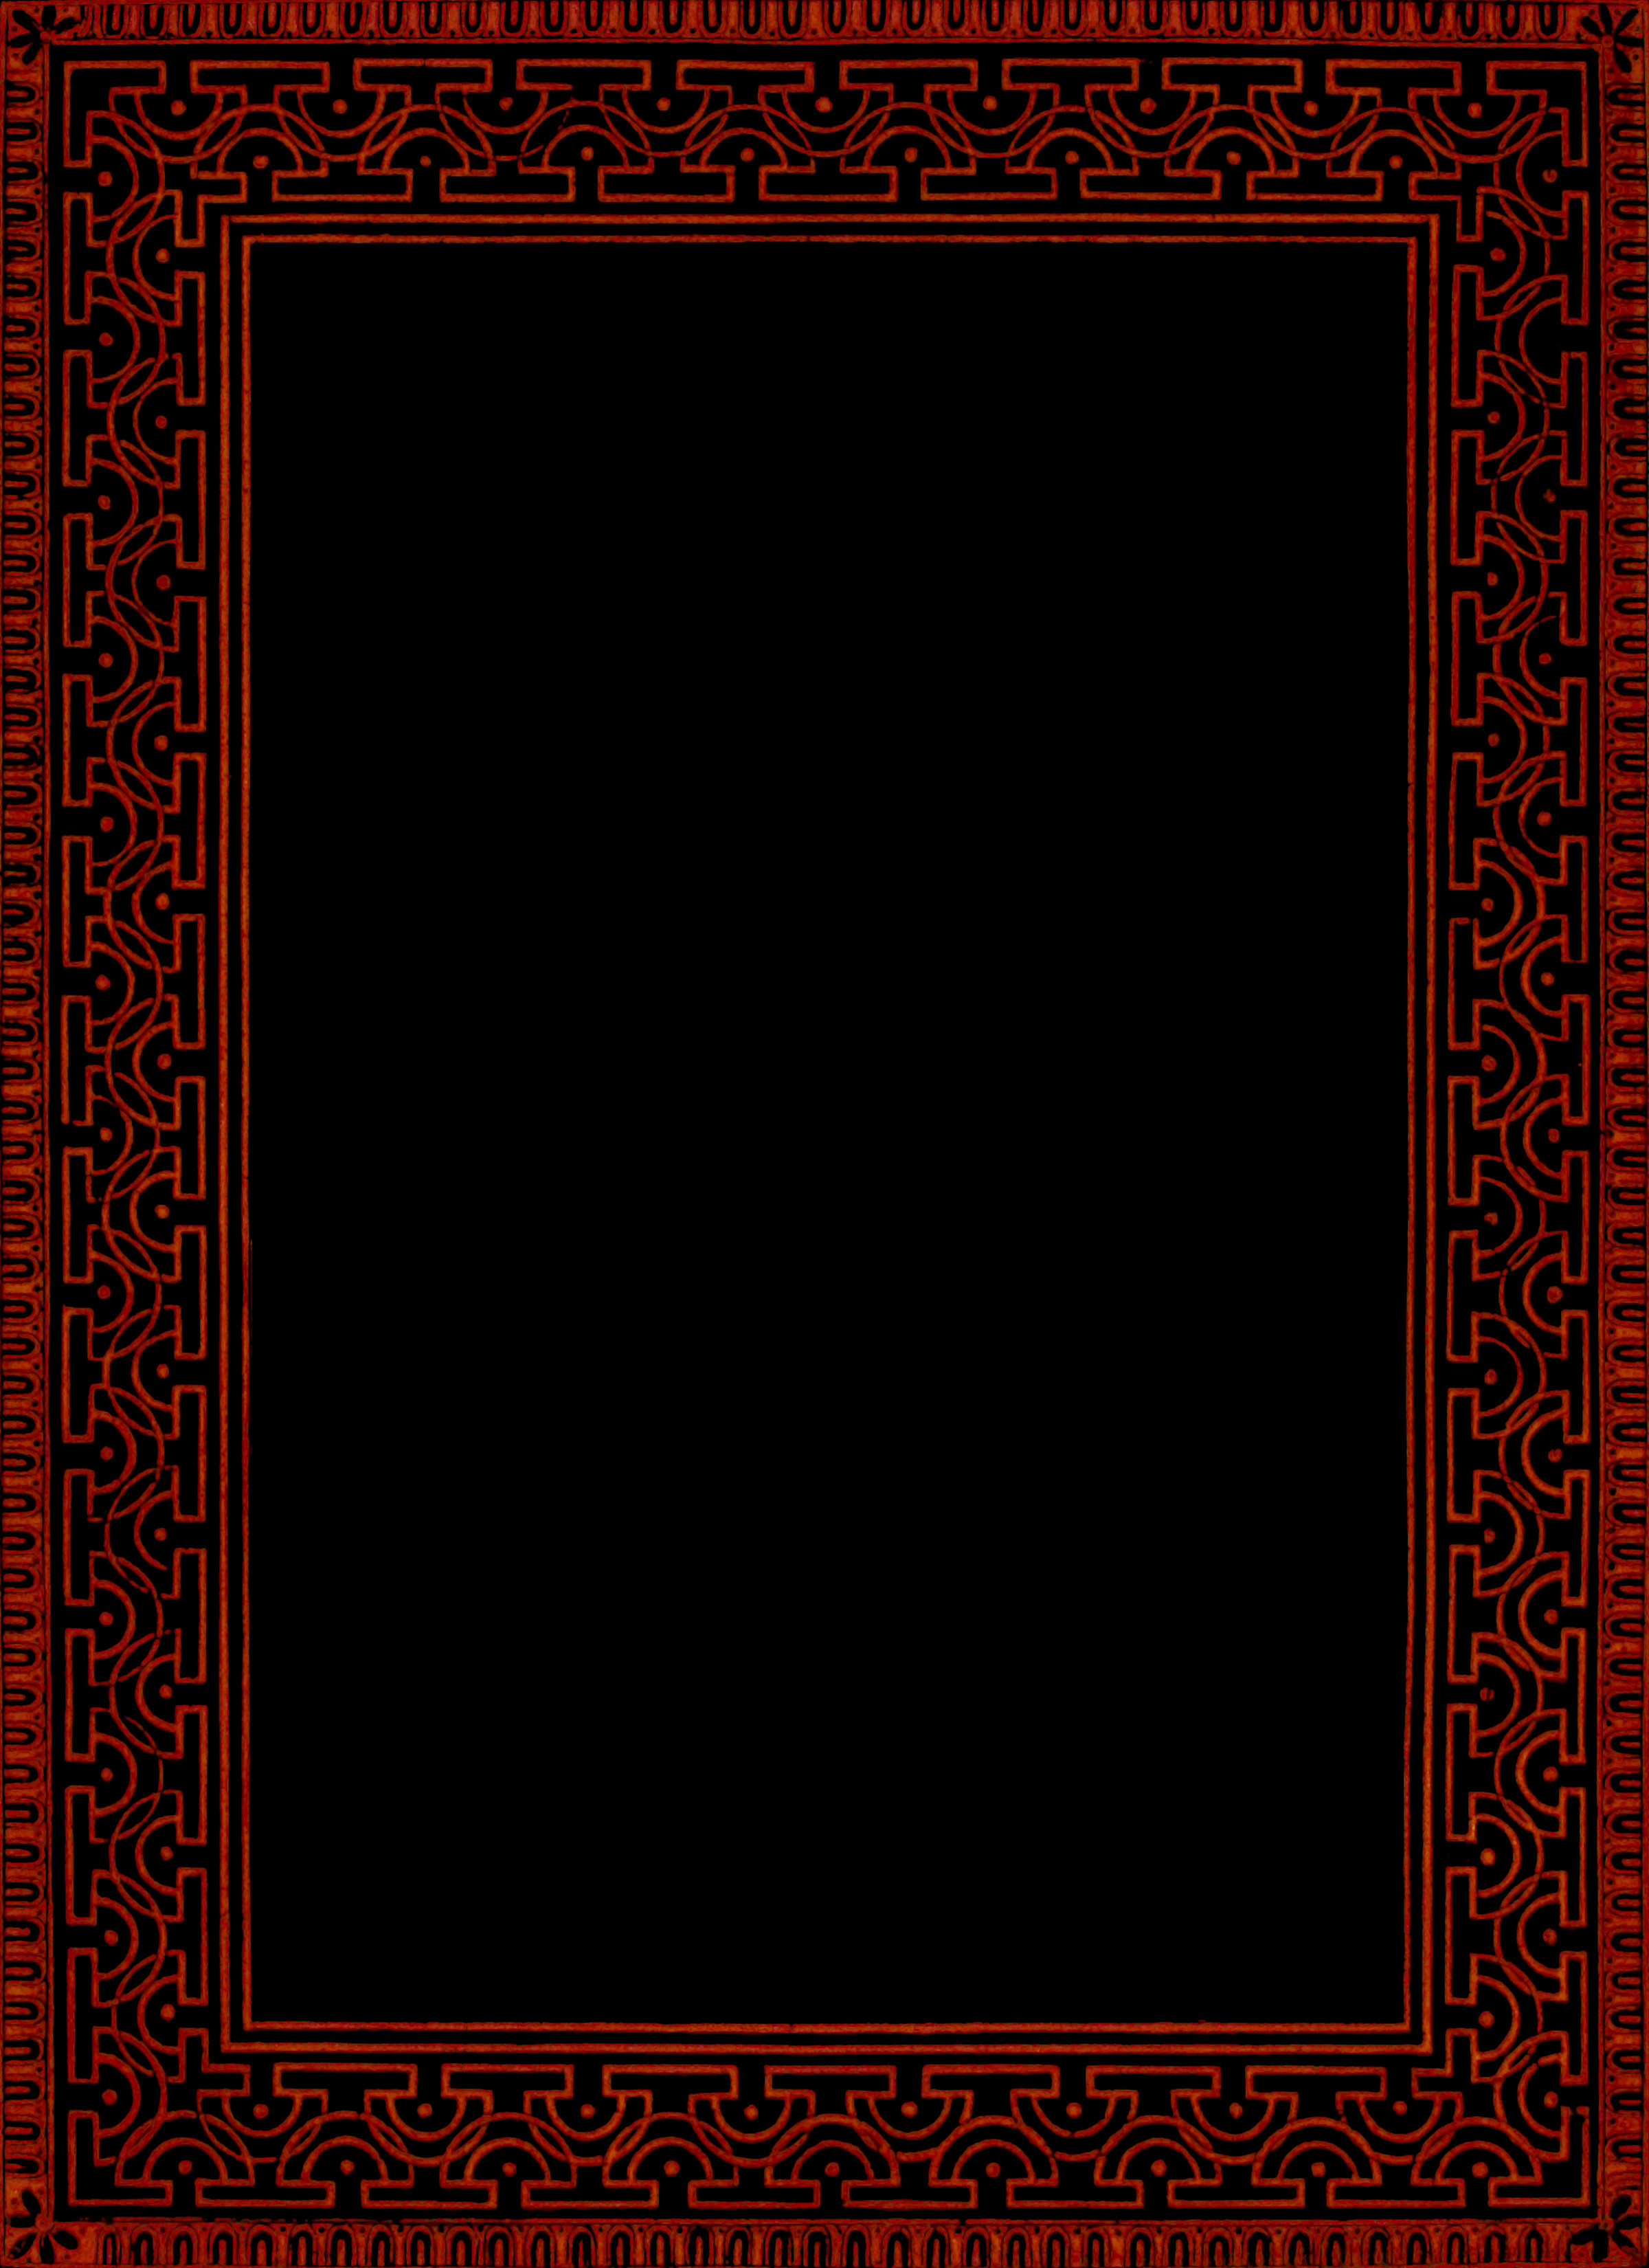
\includegraphics[width=\paperwidth,height=\paperheight]{customborder-greek.jpeg}}

\renewcommand\thefootnote{{\bfseries\color{White}{\arabic{footnote}}}}
\let\oldfootnote\footnote
    \renewcommand{\footnote}[1]{\oldfootnote{{\normalsize\bfseries\color{White}#1}}}
\begin{titlepage} % Suppresses headers and footers on the title page
	\centering % Centre everything on the title page
	%\scshape % Use small caps for all text on the title page

	%------------------------------------------------
	%	Title
	%------------------------------------------------
	
	\rule{\textwidth}{1.6pt}\vspace*{-\baselineskip}\vspace*{2pt} % Thick horizontal rule
	\rule{\textwidth}{0.4pt} % Thin horizontal rule
	
	\vspace{0.5\baselineskip} % Whitespace above the title
	
	{\scshape\Huge Der Omphalosgedanke \\bei verschiedenen Völkern, \\besonders den semitischen}
	
	\vspace{1\baselineskip} % Whitespace above the title

	\rule{\textwidth}{0.4pt}\vspace*{-\baselineskip}\vspace{3.2pt} % Thin horizontal rule
	\rule{\textwidth}{1.6pt} % Thick horizontal rule
	
	\vspace{0.5\baselineskip} % Whitespace after the title block
	
	%------------------------------------------------
	%	Subtitle
	%------------------------------------------------
	
        {\scshape Ein Beitrag zur vergleichenden Religions-Wissenschaft, Volkskunde und Archäologie} % Subtitle or further description
	
	\vspace*{0.5\baselineskip} % Whitespace under the subtitle

        {\scshape Von \Large Dr. Wilhelm Heinrich Roscher}

	\vspace*{0.5\baselineskip} % Whitespace under the subtitle

        {\scshape\small Mit 15 Figuren im Text}

	\vspace{0.25\baselineskip}


        %------------------------------------------------
	%	Editor(s)
	%------------------------------------------------

        \begin{figure}[H]
        \centering
        \includegraphics[width=0.45\textwidth,keepaspectratio]{figs/cover-invert.png}
        \end{figure}

	\vspace{0.25\baselineskip}

	{\small\scshape Leipzig 1918}
	
	{\small\scshape{Bei B. G. Teubner}}
 
	\vspace{0.5\baselineskip} % Whitespace after the title block

        \scshape Internet Archive Online Edition  % Publication year
	
	{\scshape\small Namensnennung Nicht-kommerziell Weitergabe unter gleichen Bedingungen 4.0 International} % Publisher
\end{titlepage}
\setlength{\parskip}{1mm plus1mm minus1mm}
\clearpage
\Large
\tableofcontents
\clearpage
\section*{Register --- Systematische Inhaltsübersicht.}
\subsection*{Vorwort.}
\subsection*{1. Der Gedanke eines Zentrums (`Nabels') der Erde bei den Völkern des Ostens.}
\subsubsection*{1. Die Chinesen.}
\subsubsection*{2. Die Turkstämme Südsibiriens.}
\subsubsection*{3. Die Inder.}
\paragraph{}
Die runde, in 7 konzentrische durch Berge und Meere voneinander getrennte \emph{dvîpa} (Inseln) zerfallende Erdscheibe der Inder (Mahâbhârata): S. 2. --- Ihr Zentrum ist Indien, dessen Mittelpunkt wieder entweder durch den Berg Meru oder durch die in Zentralindien gelegene Stadt dos Vikramâditya Uggajini (Ozene, Asin) gebildet wird: S. 2. --- Diese Vorstellung von der zentralen Lage und dem Meridian von Ozene-Asin ist im 13. Jahrh. auch in die geographische Literatur der Araber und aus ihr in die des christlichen Mittelalters übergegangen: S. 3. --- Auch die Insel Zeylon mit ihrem Adampik und die rätselhafte vom Istrier Aithikos erwähnte Insel Syrtinice scheinen in diesen Zusammenhang zu gehören: S. 5.

\subsubsection*{4. Die Assyrer und Babylonier.}
\paragraph{}
Der berühmte arabische Geograph Ja'kūbī erklärt den `Irāk (= Mesopotamien und Chaldaea) für den `Nabel' der Welt und Baghdad, nicht Mekka oder Jerusalem, wieder für die Mitte des `Irāk. Das erklärt sich höchst wahrscheinlich aus altbabylonischer Vorstellung, weil Baghdad in unmittelbarer Nähe des alten Babylon gelegen ist: S. 8. --- Babylon erscheint als ὀ. γῆς auch in der Sage vom Turmbau zu Babel: S. 9. --- Brief Prof. J. Hehns (Würzburg) mit weiteren Gründen für die Annahme, dass Babylon das Zentrum der Erde war: S. 10. --- Das Gleiche scheint nach Aithikos auch von Ninive zu gelten: S. 11.

\subsection*{2. Der Omphalosgedanke bei den Juden.}
\subsubsection*{1. Jerusalem als Nabel der Erde (vgl. Omphalos S. 24 ff. u. Neue Omphalosstudien S. 15 f.).}
\paragraph{}
Wesentliche Vermehrung des Zeugnismaterials durch Wensincks und Klameths Arbeiten: S. 12. --- Die ältesten literarischen Belege finden sich bei Jesaias 2, 2 und Ezechiel 5, 5: S. 13. --- Über die Vorstellung, dass Jerusalem nicht bloß die zentralste, sondern auch die höchstgelegene Stadt der Welt sei: S. 13. --- Der Stein Schetija als ὀμφαλὸς γῆς und Ausgangspunkt der Weltschöpfung: S. 14. --- Die Präexistenz dieses Steines und des Heiligtums in Jerusalem nach jüdischen, syrischen und arabischen Quellen: S. 15. --- Der Hauptgrand für diese Anschauung liegt in der Vergleichung des embryonalen Nabels mit dem Nabel der Welt oder der Erde: S. 16. --- Zeugnisse für Jerusalems Bedeutung als Erdnabel aus dem Buche Henoch, dem Talmud und Midrasch: S. 17. --- Zeugnisse aus dem christlichen Mittelalter: die Kreuzprobewunderlegende, das Zeugnis des Adamnanus (Arculfus), des Baeda, Victorinus Pictabionensis, des Typikon (vor 720): S. 18. --- Das noch heute in der griechischen Kathedrale bestehende Denkmal der Erdmitte: S. 23. --- Die mittelalterlichen Weltkarten mit Jerusalem als Mittelpunkt: S. 23.

\subsubsection*{2. Der Omphalos in der Adamlegende.}
\paragraph*{1. Die Adamlegende von Golgotha.}
Das Zeugnis des äthiopischen Adambuches: S. 25. --- Adams Grab im Golgothafelsen unterhalb des Ortes der Kreuzigung: S. 26. --- Das Zeugnis der syrischen Spelunca thesaurorum (Schatzhöhle): S. 27. --- Die Zeugnisse des Origenes, Athanasius, Ambrosius, Basilius: S. 28. --- Sie alle machen sehr wahrscheinlich, dass die Adamlegende von Golgotha jüdischen, vorchristlichen Ursprungs ist, aber später von den Juden nach Hebron verlegt wurde: S. 33. --- Die Zeugnisse für die Sage, dass Adam auf Golgotha auch erschaffen worden sei: S. 33.

\paragraph*{2. Die Adamlegende von Zion und Morija.}
Sie unterscheidet sich von der auf Golgotha lokalisierten Legende dadurch, dass für sie mehr das Motiv der Erschaffung, als dass der Bestattung Adams in Betracht kommt: S. 34. --- Zeugnisse des Rabbi Elieser und der Μικρὰ Γένεσις: S. 34. --- Spätere Übertragung dieser Sage auf Mekka: S. 36. --- Verlegung des Paradieses in die Nähe von Zion und Morija nach späteren jüdischen Quellen, weil das Paradies ebenso wie Jerusalem zugleich das Zentrum und die höchste Erhebung der Erdscheibe bedeutet: S. 36.

\paragraph*{3. Adam und Eva in Hebron bestattet.}
Merkwürdiger Widerspruch der Zeugnisse des Hieronymus, der zuerst für Golgotha, später für Hebron ein- getreten ist: S. 40. --- Weitere Zeugnisse der späteren jüdischen Literatur (Sota, Erubin, Baba batra usw.): S. 41. --- Das `Himmelstor' zu Hebron und `die über Hebron liegende himmlische Gottesstadt': S. 44. --- Dies alles legt die Vermutung nahe, dass Hebron in ältester Zeit auch den Anspruch erhoben hat, ebenso wie Jerusalem und Sichem, der ὀμφαλὸς γῆς zu sein: S. 45.

\paragraph*{4. Die Adamlegenden von Babylon und Damaskus.}
\subsection*{3. Weitere ὀμφαλοὶ γῆς in Palästina.}
\subsubsection*{1. Sichem und Garizim (samaritanische Überlieferung).}
\paragraph{}
Hohes Alter des Kultes von Sichem, der schon in der kanaanäischen Urzeit ein hochheiliger Ort gewesen sein muss: S. 49. --- Sichem als Konkurrent Jerusalems zur Zeit der Samaritaner: S. 50. --- Der Jehovatempel auf dem Berge Garizim als Gegenstück zum Tempel Jerusalems und als Erdnabel, als welcher der Garizim auch schon Richter 9, 37 (`Nabel des Landes') erscheint: S. 51. --- Weitere Zeugnisse aus der talmudischen und christlichen Literatur, wonach der Garizim von der Sintflut nicht betroffen und der aus Ev. Joh. 4 bekannte Jakobsbrunnen geradezu als `umbilicus terrae nostrae habitabilis' mit einer eigentümlichen, auch für andere umbilici terrae charakteristischen Begründung angesehen wurde: S. 52.

\subsubsection*{2. Bethel.}
\paragraph{}
Auch Bethel war seit der kanaanäischen Urzeit ein hochheiliger Ort und die Stätte, wo Jakob im Traume die `Himmelsleiter' erblickte, es galt für `den Wohnsitz Gottes und die Pforte des Himmels' (Gen. 28, 11 ff.): S. 54. --- Dass der daselbst von Jakob errichtete Denkstein wahrscheinlich ein ὀμφαλὸς γῆς gewesen ist, geht aus späteren jüdischen und christlichen Überlieferungen hervor, die geradezu Bethel als `Mittelpunkt der Erde' und den Denkstein des Jakob als `Grundstein der Erde' und `Nabel der Welt,' d. h. als Parallele zum Stein Schetija im Heiligtum Jerusalems, bezeugen: S. 56.

\subsection*{4. Mekka als Nabel der Erde.}
\paragraph{}
Zwar haben Mohammed und seine ältesten Anhänger noch Jerusalem als Mittelpunkt der bewohnten Erde angesehen, aber früh schon kam im Islam die Ansicht auf, dass Mekka und speziell die Ka'aba mit dem heiligen schwarzen Stein den Nabel der Erde darstelle: S. 57. --- Übertragung altjüdischer auf Jerusalem bezüglicher Vorstellungen auf Mekka nach arabischen, von Wensinck gesammelten Zeugnissen: S. 58. --- Altarabische Weltkarten mit Mekka als Zentrum: S. 58. --- Die Vorstellung, dass Mekka der höchstgelegene Ort auf der Erde und deshalb von der Sintflut nicht berührt worden sei: S. 59. --- Die Präexistenz Mekkas und der Ka'aba: S. 60. --- Übertragung der Legenden von Adam und Abraham nach Mekka: S. 60. --- Das Grab Evas zu Dschedda als Nabel der Erde: S. 61.

\subsection*{5. Der Omphalos von Athen und Eleusis.}
\paragraph{}
Der von den Peisistratiden gestiftete Zwölfgötteraltar als ἄστεος ὀμφαλὸς θυόεις nach Pindar: S. 62. --- Athen als ὀμφαλὸς (μέσον) τῆς Ἐλλάδος καὶ πάσης οἰκουμένης nach Xenophon de vect. 1, 6 und Aristeides Panath. 99: S. 62. --- Weitere Zeugnisse für denselben Gedanken liefern uns zwei schöne, neuerdings an der Stätte des eleusinischen Telesterions aufgefundene Pinakes und drei auf die eleusinischen Gottheiten (Mysterien) bezügliche Vasenbilder, die sämtlich einen deutlichen Omphalos zur Bezeichnung des Ortes, wo die heilige Handlung stattfindet, zur Darstellung bringen: S. 64.

a. Der Ninnion-Pinax: S. 64. --- b. Die Vase von Sta Maria di Capua: S. 68. --- c. Der boiotische Teller mit der vor einem `Omphalos' thronenden Demeter oder Persephone: S. 70. --- d. Die in Kreta gefundene attische Vase des Zentralmuseums in Athen Nr. 1442. S. 72. --- e. Der zweite im Raume des eleusinischen Telesterions (zusammen mit dem unter a behandelten) gefundene Pinax: S. 73.

Schlussfolgerung: Im Hinblick auf diese 5 monumentalen Zeugnisse kann die einstige Existenz eines richtigen Omphalos im Kult der eleusinischen Gottheiten nicht mehr bezweifelt werden: S. 75. --- Dass es sich aber im Grunde um einen ὀμφαλὸς γῆς im eleusinischen Mysterienkult handelt, folgt mit größter Wahrscheinlichkeit aus der Sage von Triptolemos, in der Athen als Mittel- und Ausgangspunkt aller auf den Segnungen des Ackerbaus beruhenden höheren Kultur und Gesittung erscheint: S. 76. --- Zeugnisse des Isokrates (Panegyr. 28 ff.) und des Platon (Menex. p. 237): S. 76. --- Dass der Erdnabel des eleusinischen Geheimkults bis jetzt nur monumental, nicht literarisch bezeugt ist, beruht auf dem außerordentlichen Einflüsse Delphis, das jede offen auftretende Konkurrenz energisch und erfolgreich zu bekämpfen wusste: S. 78.

\subsection*{6. Die Ägypter.}
\paragraph{}
Der kürzlich im Orakeltempel des Amon von Napata (Nubien) ausgegrabene und von Griffith im Journ. of egypt. Archaeol. 3 (1916) 255 ff. besprochene und veröffentlichte Omphalosstein: S. 79. --- Er bestätigt die Nachricht des Curtius Rufus (4, 7), wonach das Idol des von Alexander d. Gr. befragten Amonorakels der Oase Siwa in Libyen "`umbilico maxime similis"' war: S. 80. --- Beide Kulte, sowohl der von Napata als auch der von Siwa, sind Ableger des thebanischen Amon, dessen Orakel ebenfalls hochberühmt war; Theben galt aber wahrscheinlich als Mittelpunkt (`Omphalos') Ägyptens: S. 81. --- Pietschmanns Auffassung des `umbilicus' von Siwa als "`Tabernakel": S. 82. --- Gegen diese Ansicht und für die Deutung als ὀμφαλός spricht erstens der Umstand, dass der Stein von Napata nicht hohl, sondern massiv ist und zweitens dass sowohl der `umbilicus' von Siwa wie der von Napata bereits einer Zeit angehören, die griechischen Einflüssen ausgesetzt war, so dass das ursprünglich mehr sack- oder schlauchähnlich gestaltete Idol von Theben später die Form des delphischen Omphalos annahm: S. 83. --- Literarische Zeugnisse für die Geltung Ägyptens als Land der Mitte (Stob. ecl. 1 p. 302 M. u. Horapoll. 1, 21 a. E.): S. 84.

\subsection*{7. Die Etrusker, Italiker und Germanen.}
\paragraph{}
Wie es scheint, weist der eigentümliche als etruskisch bezeichnete Ritus bei der Gründung von Städten, insbesondere die Anlage eines sogen. `mundus' im geometrischen Zentrum des Stadtplanes auf die einstige Existenz des Omphalosgedankens auch bei den Italikern hin: S. 86. --- Die runde Form dieses `\emph{mundus}' und die ebenfalls in der Hauptsache runden Stadtmauern und Stadtgräben, die dem runden Horizont (Himmel) oder dem \emph{orbis terrarum} entsprechen, scheinen anzudeuten, dass Cato b. Fest. p. 154 Recht hat mit seiner Erklärung: `Mundo nomen impositum est ab eo mundo qui supra nos est [d. h. dem caelum, Ὄλυμπος]: forma enim eius est, ut ex his, qui intravere cognoscere potui, adsimilis illi [also rund und gewölbt]: S. 88. --- Wahrscheinlich ist `\emph{mundus}' in diesem Falle ein euphemistischer Ausdruck für die "`untere Welt"' oder "`Unterwelt,"' d. h. die Welt der abgeschiedenen Geister (manes): S. 89. --- Eine treffliche Parallele zum italischen "`mundus"' bildet der `\emph{Dillestein}' der Germanen, der dieselben Beziehungen zum Totenreiche besitzt und zugleich das Zentrum der Erde bildet: S. 89.

\subsection*{8. Der Omphalosgedanke bei den Kelten.}
\paragraph{}
Die von dem französischen Keltologen Loth hervorgezogenen Zeugnisse Cäsars (de bell. Gall. 6, 13) und des Giraldus Cambrensis Topogr. Hibern. 3, 4: S. 91. --- Das Zeugnis der Aventure de Lludd et Llevelys: S. 92. --- Weitere Belege für die einstige Existenz des Omphalosgedankens bei den alten Kelten: S. 93.

\subsection*{9. Der Erdnabel der Luiseño-Indianer Kaliforniens.}
\subsection*{10. Nachträge.}
\clearpage
\section*{Vorwort.}
\paragraph{}
Als ich vor drei Jahren das Schlusswort zu den `Neuen Omphalosstudien' schrieb, da war ich zwar, wie dieses beweist (S. 70 f.), weit davon entfernt zu glauben, dass nunmehr das gesamte zum Omphalosproblem gehörige Material von mir gesammelt und kritisch verarbeitet worden sei, aber ich hatte damals noch keine Ahnung, wie schnell und in welcher Fülle mir neuer Stoff aus allen möglichen Weltgegenden zu neuer Bearbeitung zuströmen würde.

Vor allem habe ich hier rühmend hervorzuheben die große in den `Verhandelingen der K. Akademie van Wetenschappen te Amsterdam (Afdeeling Letterkunde Nieuwe Reeks Deel 17 No. 1)' im Oktober 1916 erschienene Abhandlung des Prof. A. J. Wensinck zu Leiden, betitelt: "`The ideas of the Western Semites concerning The navel of the earth"' (12 u. 65 S. Lex. 8°). Angeregt durch meine Omphalosstudien hat Wensinck es unternommen, alle zum Omphalosgedanken gehörigen Stellen aus der Literatur der Hebräer, Aramäer (Syrer usw.) und Araber systematisch zu sammeln und zu erläutern. Ein kompetenter Beurteiler seiner Arbeit, Prof. Brockelmann in Halle a./S., hat bei der Lektüre den Eindruck gewonnen, dass, wenn auch bei der ungeheuren Ausdehnung namentlich des arabischen Schrifttums erschöpfende Vollständigkeit nie zu erreichen ist, Wensinck doch nichts Wesentliches übersehen haben dürfte.\footnote{Vgl. Brockelmanns Anzeige im Literar. Zentralbl. 1917 Sp. 1224 f.} Ich habe natürlich alles mir von Wensinck für Jerusalem, den Garizim und Mekka dargebotene Zeugnismaterial dankbar verwertet, durch Vergleichung passender Analogien erläutert und ergänzt und glaube durch Einordnung der wichtigsten Einzelergebnisse Wensincks in den größeren Rahmen meiner Arbeit allen vergleichenden Religionsforschern, die sich für das Ganze der Omphalosidee interessieren, einen Dienst erwiesen zu haben.

Ganz Ähnliches gilt auch mutatis mutandis von der gründlichen in den von Meinertz herausgegebenen `Neutestamentlichen Abhandlungen' (5, 1) 1914 erschienenen Untersuchung Dr. Gust. Klameths, welche den Titel führt: "`Die neutestamentlichen Lokaltraditionen Palästinas in der Zeit vor den Kreuzzügen."' Auch Klameth will in den beiden Abschnitten über die Golgothatraditionen (S. 88 ff.) und über das Grab Adams im Golgothafelsen (S. 106 ff.) meine Omphalosstudien von seinem Standpunkte aus tunlichst ergänzen und weiterführen, und ich muss auch ihm gegenüber dankbar anerkennen, dass es ihm in vollem Maße gelungen ist, diese seine Absicht zu verwirklichen.

Nur mit vieler Mühe ist es mir endlich mit Hilfe des mir befreundeten Prof. Waser in Zürich geglückt, der ebenfalls durch meine Omphalosstudien angeregten Arbeit des französischen Keltologen Prof. Loth in Paris habhaft zu werden, die er unter dem Titel `L'omphalos chez les Celtes' in Band 17 S. 193---206 der Revue des Études Anciennes (Jahrg. 1915) herausgegeben hat. Da diese Revue schon an und für sich in Deutschland wenig verbreitet und bekannt und zudem infolge des Weltkrieges überaus schwer zugänglich ist, so denke ich durch kurze Mitteilung der darin enthaltenen Resultate und vor allem durch Beigabe der Abbildungen mehrerer wirklicher oder problematischer Omphaloi der alten Kelten den deutschen Mitforschern auf den Gebieten der Volkskunde, Prähistorie und Archäologie einen willkommenen Dienst geleistet zu haben.

Aber auch durch briefliche Mitteilungen und Anregungen verschiedener Art bin ich von Seiten befreundeter Forscher in erfreulichster Weise unterstützt worden. Vor allem gedenke ich hier mit lebhaftem Danke der drei Ägyptologen Borchardt-Berlin, G. Roeder-Hildesheim und Sethe-Göttingen, die mir höchst wertvolle Mitteilungen über den kürzlich von Griffith in Napata (Nubien) ausgegrabenen Omphalos des dortigen Amonorakels, der den von Curtius Rufus erwähnten \emph{umbilicus} des Amontempels in der Oase Siwa bestätigen und erklären hilft, zur Verfügung gestellt haben.

Ebenfalls durch briefliche Mitteilung wichtigen Zeugnismaterials aus dem Bereiche der späteren jüdischen Literatur haben sich Prof. Dr. Winter in Dresden und Dr. M. I. Berdyczewski (bin Gorion) in Berlin-Friedenau, der Herausgeber der `Sagen der Juden' (Frankfurt a. M. 1913 ff.) und der unter dem Titel: `Der Born Judas' (2 Bde. Leipz. 1916) erschienenen Sammlung, auch um diese Fortsetzung der Omphalosstudien verdient gemacht.

Alle übrigen Gelehrten, die mich durch Anregungen und Mitteilungen verschiedener Art zu Dank verpflichtet haben, werden `suo quisque loco' von mir genannt werden.

Hierzu kommen natürlich noch zahlreiche Funde literarischer und monumentaler Art, auf die ich durch eigene Nachforschungen und Studien geführt worden bin. So stieß ich z. B. bei der Lektüre von Radloffs Proben der Volksliteratur, der türkischen Stämme Südsibiriens auf die wichtige Nachricht, dass auch diese Völker die Vorstellung von einem in ihrem Gebiete befindlichen Erdnabel haben, als welchen sie einen `kupfernen Pfeiler' (= ὀμφαλός) ansehen. Ferner ist es mir, hoffe ich, jetzt auch gelungen, in Kap. 5 mit Hilfe von 5 in den letzten Jahren entdeckten und veröffentlichten Monumenten (2 Votivtafeln [Pinakes] und 3 Vasenbildern) zu beweisen, dass ebenso wie Delphi, Delos, Paphos, Branchidai auch Athen-Eleusis, wenigstens im eleusinischen Mysterienkult, den Anspruch erhoben hat, der ὀμφαλὸς γῆς zu sein. Der auf den gedachten Pinakes und Vasen erscheinende deutliche Omphalos, den man bisher irrtümlich für den `delphischen' gehalten hat, lässt keine andere Deutung zu als die, dass er das Wahrzeichen der von Athen-Eleusis als Zentrum ausgegangenen und über die gesamte Oikumene durch Triptolemos verbreiteten Segnungen des Ackerbaus und der auf ihm beruhenden Gesittung und höheren Kultur sein sollte. --- Auch für das Verständnis des in den geometrischen Zentren der etruskischen und italischen Städte angelegten kreisrunden sogenannten "`\emph{mundus}"' hoffe ich nunmehr die richtigen Gesichtspunkte gewonnen zu haben.

Dass durch die Einordnung so vieler neuer, teils von andern, teils von mir selbst gesammelter Zeugnisse in einen gemeinsamen Rahmen das, wie man jetzt sieht, den ganzen "`orbis terrarum"' erfüllende Omphalosproblem nicht unwesentlich gefördert worden ist, dürfte mir wohl von jedem billigdenkenden Beurteiler zugestanden werden.

Auch diesmal wieder beginnen wir unsere Wanderung im fernen Osten, um sie im äußersten Westen zu beschließen.

Dresden-A., Febr. 1918.
\clearpage
\vspace*{\fill}
\begin{figure}[H]
\centering
\includegraphics[width=0.55\textwidth,keepaspectratio]{figs/forward-invert.png}
\caption*{\bfseries Der jetzige in der griechischen Kathedrale befindliche Omphalos von Jerusalem (nach `Omphalos' Taf. 9, Fig. 3).}
\end{figure}
\vspace*{\fill}
\clearpage
\section{Der Gedanke eines Zentrums (`Nabels') der Erde bei verschiedenen Völkern des Ostens.}
\subsection{Die Chinesen.}
\paragraph{}
Omphalos S. 20 f. habe ich auf Grund der außerordentlich wertvollen Mitteilungen A. Forkes den Omphalosbegriff der Chinesen, der wohl einmal eine gründliche Untersuchung verdiente, kurz dargestellt. Ich verweise jetzt in dieser Hinsicht auf Richthofen, China 1, Berl. 1877 S. 311: `Den [Berg] Waifang suchen sie [die Kommentatoren des Yü-king] in dem gegenwärtigen Sung-shan, einem schönen, in ungefähr 8000 Fuß gipfelnden Gebirgsstock, welcher sich südöstlich von Ho-nan-fu erhebt und eine isolierte Stellung einnimmt. Er wurde in späterer Zeit als der fünfte unter die heiligen Berge von China aufgenommen und auch Tshung-shan oder Berg der Mitte genannt, indem er als der Mittelpunkt des Reiches [d. i. des Reiches der Mitte] betrachtet wurde.' Vgl. auch V. Andrian, D. Höhencultus asiat. u. europäischer Völker. Wien 1891 S. 166.

\subsection{Die Turkstämme Südsibiriens.}
\paragraph{}
Zu den Völkern des Ostens, welche einen Erdnabel in ihrem Bereiche angenommen haben, gehören auch die Turkstämme Südsibiriens. Nach Radloff, Proben der Volkslitteratur der Türk. Stämme Südsibiriens 2 S. 242 ff. haben diese Stämme die Vorstellung von einem durch `einen kupfernen Pfeiler' [also einen kupfernen Omphalos] bezeichneten "`Nabel der Erde,"' den unter allen `Helden und Starken' nur der `neunjährige Held Kara Par'\footnote{Zu den überaus zahlreichen bei den noch dem alten Schamanenglauben huldigenden Stämmen Südsibiriens vorkommenden typischen Zahlen, darunter massenhaft auftretenden Triaden, Hexaden, Heptaden, Enneaden und Tessarakontaden, s. meine Bemerkungen in `Die Zahl 50 in Mythus, Kultus, Epos und Taktik d. Hellenen u. and. Völker' S. 113 f.} zu heben und herauszuziehen vermag.

\subsection{Die Inder.}
\paragraph{}
Auch das Zeugnismaterial für die einstige Existenz des Omphalosgedankens bei den Indern (s. Omphalos S. 22 u. Neue Omph. Stud. S. 14 u. 72 f.) kann ich jetzt mit Hilfe von Lassens Indischer Altertumskunde und Peschels Abhandlungen z. Erd- u. Völkerkunde 1 Leipz. 1877 nicht unwesentlich vermehren.

Nach Lassen a. a. O. 4 S. 59 besteht die Erde nach der vorherrschenden Ansicht der Inder aus sieben durch Berge und Meere voneinander getrennten \emph{dvîpa} oder Inseln.\footnote{Über die Heiligkeit der Siebenzahl bei den Indern s. meine Abhandlungen `Die enneadischen u. hebdomadischen Fristen u. Wochen d. ältest. Griechen' S. 34 f. und `Die Sieben- u. Neunzahl im Kultus u. Mythus d. Griechen' S. 87.} Sie hat nach Albîrûni eine runde Gestalt (orbis terrarum) und ist von einem Meere (vgl. den Okeanos der Griechen!) umflossen. Sie ist in sieben \emph{dvîpa} geteilt, welche durch Ozeane in der Weise voneinander geschieden sind, dass jene wie Halsbänder sich umschließen und jede Insel und jedes Meer einen größeren Umfang haben, je weiter sie vom Mittelpunkte entfernt sind. Die mittlere Insel heißt Gambûdvîpa; sie ist die vornehmste von allen, und zu ihr gehört Indien. Die früheste Beschreibung der 7 dvîpa mit ihren Meeren und Gebirgen findet sich im Mahâbhârata (älter als das 4. Jahrh. nach Chr.). Auch nach dem kosmographischen System der Purâna bildet die Gambûdvîpa die Mitte des indischen Weltsystems, und deren Zentrum wieder der goldene Berg Meru (Lassen a. a. O. S. 60; vgl. N. Omphalosstudien S. 72), während nach noch älterer Ansicht der Meru (= Himalaya?) nicht im Zentrum der Erde sondern im äußersten Norden liegt (Lassen a. a. O. 1 S. 847).

Für die letztere Vorstellung scheinen auch die eigentümlichen Überlieferungen zu sprechen, welche sich auf die indische Stadt Uggajini = Ozene (= Oudjein, Ujjain, Oojein, Asin, Arin, Aryn, Arim) beziehen. Dieses Ozene (Ptolem. u. Arrian) war die Hauptstadt von Larika (= Malva), der bekannten Landschaft im Zentrum von Indien,\footnote{Vgl. darüber: Lassen a. a. O. 3, 148, 4. 171. Encyclopaedia Britannica 15, 346 c. 23, 719: In ancient times Ujjain was the great and famous capital of Málvá, one of the seven sacred cities of the Hindus, and the spot which marked the first meridian of Hindu geographers.} ein uralter noch bis in prähistorische Zeiten zurückreichender Sitz der Wissenschaften und Künste, besonders berühmt als Residenz des großen Königs Vikramâditya, des erlauchten Förderers der Astronomie (Astrologie?) und Gründers mehrerer Sternwarten, besonders der von Ozene.\footnote{Benfey in Ersch u. Grubers Encyclopädie 2, 17 S. 269 b (Artikel `Indien'). Encycl. Britann. 21, 283. 15, 346 c. --- Vgl. Curt. Ruf. 8, 9, 33: Illi, qui in urbibus publicis moribus degunt, siderum motus scite spectare dicuntur et futura praedicere.} Mit dieser Bedeutung von Ozene hängt es offenbar zusammen, wenn berichtet wird, dass das im Zentrum von Mittelindien (Malva, Larika) gelegene Uggajinî den `Omphalos' der altindischen Weltkarte gebildet habe, denn es heißt ausdrücklich, ihr erster Meridian sei von Lankâ (= Zeylon) aus durch Uggajinî und die Festung Koshtaka und die Quellen der Jamunâ nach dem Berge Meru, der sonach wohl unzweifelhaft im Norden zu denken ist (= Himalaya), gezogen worden.\footnote{Lassen a. a. O. 4 Anhang S. 59, der diese Bestimmung dem ersten wissenschaftlichen Astronomen der Inder, dem Ârjabhaṭṭa, zuschreibt.} Damit hängt es nun ganz offenbar zusammen, wenn ein arabischer Kosmograph des 13. Jahrhunderts (Reinaud, Aboulféda, Introd. p. 243; vgl. Peschel a. a. O. S. 48 f. in seinem schönen Aufsatze über `Die Kuppel von Arin' = Ozene) sagt: `Unter dem Aequator, in der Mitte der Welt, da wo wir keine Breitengrade zählen, liegt ein Punkt, der 90° von jedem der 4 Cardinalpunkte entfernt liegt. Hier findet sich der Punkt, der "`die Kuppel von Azin oder von Arin"' heißt. Dort ist ein großes, hohes und unzugängliches Schloss. Nach Ibn-al-Araby dient es bösen Geistern /um Aufenthalt und als Thron dem Iblis (Teufel).'\footnote{Unter dem `Thron des Iblis' hat man wahrscheinlich den Tempel oder Sitz eines altindischen Gottes zu verstehen, der in Ozene hoch verehrt wurde. Die streng monotheistischen Araber machten natürlich den Sitz des `Teufels' daraus.} Peschel fügt hinzu: `Columbus spricht davon in seinem Bericht an den spanischen König über seine dritte Reise und sagt: Ptolemäus und andere hielten die Welt für kugelförmig, weil sie glaubten, diese Hemisphäre (Amerika) sei gerundet, wie jene wo sie lebten, und deren Mittelpunkt sich auf der Insel Arin befindet, welche unter dem Äquator, zwischen dem arabischen und persischen Meerbusen liegt.'\footnote{Al. v. Humboldt bezeichnete im Jahre 1837 diese Bestimmung als ein Rätsel, dessen Lösung seit Columbus verloren gegangen sei (Peschel a. a. O.).}

Weiter führt Peschel den Irrtum Santarems, Essai 3 p. 311 (1848) an, dass die älteste abendländische Karte, welche Aryn verzeichne, sich als Beigabe zur Imago mundi des Kardinals Alliacus vom Jahre 1410 finde,\footnote{Vgl. über ihn auch Marinelli, D. Erdkunde b. d. Kirchenvätern, deutsch von Neumann. Leipz. 1884 S. 76 A. 45.} und verweist demgegenüber auf eine Entdeckung von Reinaud 1852, bestehend in einer Weltkarte des 12. od. 13. Jahrhunderts, einem Werke des Peter Alfons (geb. 1062) mit einer Planisphäre wo die `civitas Aryn' in der Mitte der Welt abgebildet ist.

Nach Al. v. Humboldt (im Examen critique) hatte Columbus auf seiner dritten Reise die Werke des Alliacus an Bord, der zweimal von Aryn spricht und beide Male (Imago mundi cap. 15 u. Cosmogr. cap. 19) den Roger Bacon (Opus majus Lond. 1733 Fol. 188 u. 195) wörtlich ausschreibt. Dieser aber versetzt die von ihm mit Syene identifizierte Stadt Arym unter den Äquator und sagt: `Dies ist die Stadt A., welche die Mathematiker in die Mitte der bewohnten Erde unter den Äquator versetzen, da sie in gleichem Abstande von Ost und West, Norden und Süden sich befindet, womit der Volksirrtum widerlegt wird, als liege Jerusalem in der Mitte der Welt' (s. unt. Kap. 2).\footnote{Vgl. Marinelli a. a. O. S. 76 Anm. 45, nach dem Alliacus Jerusalem wenigstens zum Mittelpunkte der Klimata machte.}

Weiter wies Reinaud (Aboulféda, Introd. p. 246) nach, dass im Occident zuerst Gerhard v. Cremona (12. Jahrh.) von Arin gesprochen hat in seiner Übersetzung der 1070 zu Toledo von Abu-Ishak-Ibrahim verfaßten astronomischen Tafeln, worin von einem `medium mundi, qui locus dicitur esse in India in civitate scilicet, quae vocatur Arin,' die Rede ist.

Wie man also heute nach dem Meridian von Paris und Greenwich rechnet, so nahmen die Araber des Mittelalters einen idealen Meridian an und ließen diesen die im Zentrum Indiens gelegene Stadt Arin berühren. In diesem Falle haben sie sich wohl sicher an die uralte Weltkarte der Inder angeschlossen, deren `Omphalos' oder Zentrum die durch König Vikramaditya mit einer hochberühmten Sternwarte versehene Stadt Odjein (= Ozene des Ptolemäus), der Mittelpunkt indischer Gelehrsamkeit um jene Zeit war, als die Araber große Eroberungen in Indien machten. Der über Odjein gezogene Meridian berührte aber zugleich die Insel Lanka (= Taprobane, Sîhala, Σάλαι, Σιμούνδου? Σαλική [Ptolem.], Sêlan, Serendiva [Ammian], Serendîb [arab.], = Σελεδίβα nach Kosmas Indikopleustes),\footnote{Vgl. Kiepert, Lehrbuch d. alt. Geogr. § 42.} d. i. Zeylon (Peschel a. a. O. S. 52).

Auf Zeylon aber waren nach der Annahme der Araber, welche sich jedoch auch hier wohl an altindische (buddhistische) Vorstellungen und Sagen angeschlossen haben dürften, die Legenden vom ersten Menschen (Adam) und vom Paradiese lokalisiert, die, wie später gezeigt werden wird, mit der Vorstellung vom Nabel der Erde untrennbar verbunden sind.\footnote{Vgl. Fabricius, Codex Pseudepigr. Vet. Testam. Hamburg 1722 2 21 ff.: Mons est in insula Zeilon totius Indiae, ut ferunt, altissimus, quem Lusitani `Pico del Adamo' appellaverunt incolarum fabulas secuti. In hoc specus quaedam, cujus in recessu Arabes cum Indis constanter tradunt Adamum fletu ac continentia culpam redemisse. Ostenditur etiam lacus quispiam parvus falsae naturae, qui ortus sit ex lachrymis Evae Abelem occisum deflentis. Magna insuper religione ab advenis visuntur vestigia Adami. --- p. 23: Indi plerumque fabulam corrumpunt, quod credi volunt Adamum in eadem insula creatum, in eadem Paradisum fuisse. Diese Lokalsage verdient gewiss eine ausführliche Untersuchung. --- S. auch Dähnhardt, Natursagen 2 S. 234 f. --- Bei dieser Gelegenheit gedenke ich noch einer wertvollen brieflichen Anregung Fr. Hommels in München, der mir am 30./6. 15 schrieb: `Der Berg Sinnalu (auf Celebes) und der Zinnalo (in Siam; vgl. N. Omphalosstud. S. 72 f.) im Zentrum der Erde gehört gewiss zum alten Namen Sinhala-dvîpa von Ceylon, den man gewöhnlich von sinha Löwe ableitet. Ceylon hieß Taprobane, was an hebr. ṭabbur = Nabel erinnert. Ich hoffe, nächstes Jahr Beiträge zum Omphalos aus altorientalischen Quellen zu veröffentlichen.'}

Vielleicht beziehen sich auf Zeylon und die diese Insel berührende Mittagslinie auch folgende Sätze des Kosmographen Aethicus, die von der sonst rätselhaften, im indischen Ozean gelegenen südlichen Insel Syrtinice (Sirtinice, Sirthnice, Sirthimice, Sirtice)\footnote{Wenn man die außerordentlich mannichfaltigen Benennungen der Insel Zeylon in Betracht zieht (s. darüber Kiepert, Lehrb. d. alt. Geogr. § 42): Ταπροβάνη (von Tâmraparnî, vulgär Tâmbapannî, dem Namen der früheren Hauptstadt), Sinhala (vulg. Sîhala, b. Ptolem. Σάλαι, Σαλική), jetzt Sêlan (vulg. Ceylon nach portugiesischer Schreibweise), Serendiva (nach persischer des Lautes l ermangelnder Aussprache) bei Amm. Marc. = Serendîb (bei den Arabern) = Σιελεδίβα (im Periplus), d. i. Sinhala + dvîpa (= Insel), so wird man es wohl nicht für unglaublich erklären, dass daraus bei Aethicus die Formen Sirtinice etc. entstehen konnten. Vgl. auch Ozene, = Uggajini = Oudjein = Asin = Arin usw.} mit einem höchsten Berge Namens Austronothius berichten (ich zitiere nach der Ausgabe von H. Wuttke, Leipz. 1854):

p. 12 Kap. 21: Lineam praemagnam tendentem ad meridiem: revera nimio frigore inculta a septentrione a<d?> meridie<m?> nimis opulentam plagam, quam umbelicum solis [orbis?]\footnote{Ich vermute ebenso wie Lelewel (s. unt.) dass statt \emph{solis}, was mir gar keinen vernünftigen Sinn zu ergeben scheint, zu lesen ist: \emph{orbis} <\emph{terrarum}>. Wie ist es aber zu erklären, dass aus \emph{orbis solis} werden konnte? Bekanntlich werden in Handschriften statt ἥλιος (sol) und σελήνη (luna) sehr oft die Zeichen $\odot$ und \leftmoon geschrieben. Das Zeichen für ἥλιος (sol) aber kann natürlich auch κύκλος oder \emph{orbis} bedeuten. So konnte ein Abschreiber leicht auf den Gedanken kommen, dass das Zeichen $\odot$ hier die Sonne bedeute, weil ihm diese Bedeutung geläufiger war. Vgl. Parthey, Zwei griech. Zauberpapyri, Abh. d. Berl. Akad. 1865 S. 172 unter ἥλιος u. S. 177 unter σελήνη. --- Derselbe Ausdruck \emph{umbelicus solis} kehrt wieder Kap. 20 p. 11 Wuttke: Sic et a meridie nimis opulentam plagam, quam umbelicum solis [= orbis?] idem chosmografus refert, temperatam et ditissimam, ventis salubrem, imbribus pinguissimis infectam. Es handelt sich in diesem Zusammenhang offenbar um Indien (vgl. p. 12, 6: e Gange hippopotamos). Unmittelbar vorher war von einer linea praemagna tendens ad meridiem, d. h. doch wohl von dem mitten durch Indien gezogenen Meridian von Ozene die Rede.} idem cosmographus refert. Dicit enim insolam meridianam Syrtinicen ad umbilicum solis [orbis?] in magnum oceanum, parvula statura, silvas et nullos accessus hominum, nisi raro, si naves vento turbatae sunt contrario.

p. 13 Kap. 23: Haec omnia de ianuis caeli et cardinibus mundi tergoque solis [?], septentrione et umbelico eius descripsit. Meridiem lineam a parte ad partem mediam mundi protelantem ab aquilone in meridiem...

Trotz der miserabeln Überlieferung und der wohl schon von Haus aus etwas unklaren Ausdrucksweise scheint, wie schon Lelewel (Géogr. du moyen âge 2 p. 8 u. p. 123) gesehen hat, die Insel Syrtinice einerseits mit einem von Norden nach Süden gezogenen Meridian, anderseits mit einem Nabel (umbilicus) der Erde in Zusammenhang gebracht zu werden, zwei wichtige Merkmale, die mit einiger Wahrscheinlichkeit nur auf das nach altindischer Anschauung unter dem Meridian von Ozene liegende Ceylon bezogen werden können.\footnote{Wuttke a. a. O. S. 12 f. ist geneigt, die Insel Syrtinice mit Réunion (Bourbon) zu identifizieren, doch steht dieser Annahme wohl die Tatsache entgegen, dass Réunion, soviel wir wissen, erst im Jahre 1505 von dem Portugiesen Mascarenhas entdeckt wurde und von dem Meridian Ozenes sowie von allen zur Zeit des Aethicus bekannten Ländern (auch von Taprobane = Ceylon; s. a. a. O. p. 14 Kap. 24) viel zu weit abliegt.} Lelewel a. a. O. S. 123 sagt darüber: `Ethicus visita le nombril de la terre ou de l'hémisphère, l'île Syrtinice, par laquelle passe d'un pole à l'autre la ligne méridionale, ou le meridien qui divise l'hémisphère et l'habitable en deux parties égales occidentale et orientale... Cette doctrine de la ligne méridionale ou du meridien qui passait par l'île (Syrtinice), qui est le siège du ciel et le nombril de la terre, vient des Grecs, mais sa confusion avec les doctrines indiennes et avec le méridien d'Oudjein est l'ouvrage des Arabes.' Auch diese Auffassung Lelewels scheint eher auf Zeylon als auf die sonst in älterer Zeit völlig unbekannte und deshalb unseres Wissens nie benannte Insel Réunion zu deuten.

\subsection{Die Assyrer und Babylonier (vgl. Omphalos S. 23 f.).}
\paragraph{}
Dass auch Ninive und Babylon sich gerühmt haben, Mittelpunkte der Erde zu sein, kann ich jetzt mit weit besseren Zeugnissen belegen als es Omphalos S. 23 f. geschehen ist. Vor allem kommt hier in Betracht der Umstand, dass, wie mir Goldziher nachweist, Ja'\d{k}ūbī, Kitāb al-boldan (Bibl. Geogr. Arab. Bd. 7 p. 233, 19 ff.) sagt, dass seine Beschreibung "`deswegen mit dem `Irā\d{k} [= `Irā\d{k}-Arabī d. i. Mesopotamien und Chaldaea] beginne, weil es die Mitte der Welt und der Nabel (surra) der Erde ist; Baghdad (in der Nähe der Ruinen von Babylon) wieder ist die Mitte vom `Irā\d{k}."'\footnote{Vgl. auch Lelewel, Géogr. du moyen âge 2, Épilogue chap. 70 p. 121: `Dans ces images rondes [gemeint sind arabische Weltkarten] on distingue une habitable dont le centre est ou Jérusalem ou les environs de Mekka, de Bagdad.' Vgl. Proleg. p. 81 (vol. 1). S. auch Jeremias, Handb. d. altor. Geisteskultur S. 56 und 189 f. (Babylon = `Mittelpunkt des himmlischen Landes').} Da nun aber die islamischen Araber (wie ich weiter unten zeigen werde) sonst meist entweder Jerusalem oder Mekka für den Nabel der Erde erklärt haben, ist es so gut wie sicher, dass Ja'\d{k}ūbī in diesem Falle einer altbabylonischen Anschauung gehuldigt hat, die sich auch sonst sehr wahrscheinlich machen lässt.

Vor allem verweise ich auf die uralte Sage vom Turmbau zu Babel und der dadurch veranlassten Spaltung der ursprünglich einheitlich gedachten Sprache, insofern hier Babylon deutlich als Zentrum der Erde und Urheimat der Menschheit erscheint. Genes. 11, 1 (Kautzsch) heißt es: `Es hatte aber die ganze Menschheit eine Sprache und einerlei Worte.' --- V. 4: `Da sprachen sie: Wohlan, wir wollen uns eine Stadt bauen und einen Turm, dessen Spitze bis an den Himmel reicht, und wollen uns ein Denkmal machen, damit wir uns nicht über die ganze Erde hin zerstreuen' (der Turm, auf dessen Spitze sich aller Wahrscheinlichkeit nach ein astronomisches Observatorium befand, sollte also zugleich das weithin sichtbare Symbol der Erdmitte und der Einheit aller Menschen sein). --- V. 6 `Und Jahwe sprach: Ein Volk sind sie und haben alle dieselbe Sprache...' V. 7: `Wohlan, wir wollen hinabfahren und daselbst ihre Sprache verwirren, so dass keiner mehr die Sprache des andern verstehen soll.' --- V. 8: `So zerstreute sie Jahwe von dort über die ganze Erde, so dass sie davon abstehen mussten, die Stadt zu erbauen.' Dass in dieser von mir absichtlich in ihrem ursprünglichen Wortlaut angeführten Legende Babylon mit seinem gewaltigen Stufenturm nur als Mittelpunkt des `Orbis terrarum' und Urheimat der gesamten Menschheit (vgl. unten das von Adam und den Orten seiner Erschaffung handelnde Kapitel!) verstanden werden kann, dürfte wohl nicht dem geringsten Zweifel unterliegen.

Herrn Prof. J. Hehn in Würzburg verdanke ich ferner folgende wertvolle briefliche Mitteilung.

"Mit dem `Omphalos' S. 23 von A. Jeremias erwähnten DUR. AN. KI weiß ich für die Omphalosvorstellung nicht viel anzufangen. Aber zur babylonischen Vorstellung von einem Weltmittelpunkt darf ich mir vielleicht erlauben, Sie an meine von Ihnen so freundlich beurteilte Studie über die Siebenzahl zu erinnern, in der die babylonischen Stufentürme als Symbole des Kosmos gedeutet sind, dessen Herrschaft dem auf der Spitze thronenden Gott zukommt (S. 15). Sollte der Thron vielleicht als Zentrum der Welt gedacht worden sein? Die Namen der Stufentürme würden dazu passen.\footnote{Dieselbe Vorstellung macht Wensinck in seiner Abhandlung `The navel of the earth' in einem besonderen Kapitel (3 E, S. 54 ff.) auch für die Westsemiten wahrscheinlich. Vgl. z. B. 1 Chron. 29, 23: `Und so saß Salomo an Stelle seines Vaters David als König auf dem Throne Jahwes' [in Jerusalem].}

Der Stufenturm Gudeas hieß (S. 8 f.) "`Haus der 7 tubugāte,"' d. h. "`Haus der 7 Welträume"' oder der Welt; der von Babel E-temen-an-ki "`Haus der Grundfeste Himmels und der Erde"' (S. 9). Der Tempel stellt also die Grundlage der Welt dar.\footnote{Eine westsemitische Parallele dazu bildet offenbar die jüdische Vorstellung vom Stein Schetija im Tempel zu Jerusalem, der zugleich als Mittelpunkt der Welt und als deren Grundstein aufgefasst wurde. Vgl. Neue Omphalosstudien S. 16 f., Feuchtwang in Monatsschrift f. Gesch. u. Wissensch. des Judentums 1910 S. 545 ff. u. 727 ob. S. auch unt. Kap. 2 A.} Ein Tempel von Kiš (Kiš bedeutet "`Gesamtheit, Welt"' und kommt mehrfach als Stadtname vor) heißt Te-an-ki-bi-da "`Grundfeste Himmels und der Erde"' (S. 10), der Tempelturm von Borsippa "`Haus der 7 Beherrscher Himmels und der Erde"' (S. 10 f.). Dass die Stufentürme Sinnbilder des Kosmos sind, scheint mir sicher; dass bei ihrer Herstellung die Vorstellung von einem Weltberge mitgewirkt hat, ist mir wahrscheinlich.\footnote{Wensinck in seiner weiter unten vielfach von mir zitierten Schrift The navel of the earth = Verhandelingen der K. Akademie van Wetenschappen. Amsterd. 1816 weist nach, dass die Westsemiten dem Nabel der Erde (Jerusalem, Mekka usw.) eine Höchstlage zuschrieben.} Der sumerische Name für Tempel ī-kur "`Berghaus"' ist auch ins Babylonische übergegangen (ekurru), viele Tempel werden als Berge bezeichnet, z. B. Ē-\b{h}ar-sag-kur-kur-ra "`Länderberg"' ist der Name des Haupttempels Assurs, und ähnliche Namen sind häufig. Der Gott Ellil-Bēl heißt kur-gal "`der große Berg."' Von hier aus ließen sich wohl die babylonischen Vorstellungen von einem Weltmittelpunkte erklären und Beziehungen zu denen anderer Völker finden, wozu Ihre sorgfältigen Sammlungen die beste Grundlage geliefert haben. Ich werde das babylonische Material einmal genauer prüfen und hoffe vielleicht darüber einmal eine Untersuchung liefern zu können."' Auch die eigentümliche Rolle, welche Babylon in der Legende von der Erschaffung Adams spielt (s. unten Kapit. 2 B 4), deutet, wie später gezeigt werden soll, darauf hin, dass es als Zentrum der bewohnten Erde angesehen wurde.

Ebenso wie Babylon (und Bagdad) scheint auch Ninive als Mittelpunkt der Erde gegolten zu haben. Dies ist mit einiger Sicherheit zu erschließen aus den leider etwas verderbten Worten des Aethicus Istricus cap. 107 p. 80 ed. Wuttke: `Assyria etenim nobilissima, purpora quidem procerior, ornata opibus omnium bonorum. Umbelicum ac medullam [meditullium?] Niniven, quam philosophus inter alias urbes moenianam Archochyram[?] vocitavit,' Vgl. dazu Lelewel, Géogr. du moyen âge 2 p. 9, der (Anm. 21) dazu bemerkt: `Fra Mauro près de ce nombril plaça le centre, le nombril de sa mappemonde (Géogr. du moyen âge 165).' Dass diese Zeugnisse für Babylon und Ninive sich gegenseitig stützen und beglaubigen, braucht kaum bemerkt zu werden. Wir werden später zu zeigen suchen, dass auch im Gebiete der Westsemiten verschiedene Städte sich die Ehre, Nabel der Erde zu sein, streitig machten, besonders Jerusalem, Sichem, Bethel, Mekka, Dschedda.
\clearpage
\section{Der Omphalosgedanke bei den Juden.}
\subsection{Jerusalem als Nabel der Erde.}
\paragraph{}
Bereits in meinen beiden ersten Abhandlungen (Omphalos S. 24 ff. und Neue Omphalosstudien S. 15 ff.) habe ich auf Grund einer Anzahl von Zeugnissen den Beweis geführt, dass Jerusalem als das Zentrum des heiligen Landes\footnote{Joseph. bell. Jud. 3, 3, 5: μεσαιτάτη τῆς Ἰουδαίας πόλις τὰ Ἱεροσόλυμα κεῖται, παρ᾽ ὃ καί τινες οὐκ ἀσκόπως ὀμφαλὸν τὸ ἄστυ τῆς χώρας ἐκάλεσαν. Ebenso schon der Aristeasbrief (um 200 v. Chr.) ed. Wendland p. 25, 8 ff.: Ὡς γὰρ παρεγενήθημεν ἐπὶ τοῦ καὶ τόπου, ἐθεωροῦμεν τὴν πόλιν μέσην κειμένην τῆς ὅλης Ἰουδαίας ἐπ᾽ ὄρους ὑψηλὴν ἔχοντος τὴν ἀνάτασιν.} seit alter Zeit auch den Anspruch erhoben hat, der Nabel der Erde zu sein. Es sei mir jetzt nach dem Erscheinen der Arbeiten von Wensinck, Klameth u. a., durch die sowohl das Zeugnismaterial als auch die Zahl der in Betracht kommenden Gesichtspunkte wesentlich vermehrt worden ist, verstattet, die ganze Frage noch einmal ausführlich zu behandeln und auf diese Weise meine früheren Darlegungen tunlichst zu ergänzen. Dabei sei jedoch vorausgeschickt, dass ich hier zunächst nur die nicht mit der Adamlegende zusammenhängenden Zeugnisse anführen und behandeln werde, während die der Adamsage angehörenden, teils aus Gründen der Methode teils um die bei der übergroßen Fülle des Materials sonst leicht entstehende Unübersichtlichkeit tunlichst zu vermeiden, einem besonderen Abschnitt (s. Kap. 2 B) vorbehalten bleiben müssen. Eine derartige kritische Sonderung bietet zugleich den nicht geringen Vorteil, dass durch sie eine Anzahl neuer Gesichtspunkte gewonnen wird, die dem Verständnis nicht bloß des Omphalosgedankens sondern auch des Schöpfungsmythus der Westsemiten zugutekommen dürften.

Zu der (Omph. S. 24) als grundlegend angeführten berühmten Stelle des Propheten Ezechiel (um 595 v. Chr,) 5, 5: `So spricht der Herr Jahwe: Dies ist Jerusalem, die ich mitten unter die Völker gestellt habe, und rings um sie her Länder'\footnote{Vgl. dazu auch Ezech. 38, 12, wo die Israeliten bezeichnet werden als `Leute, die auf dem Nabel der Erde wohnen,' und Hieronymus zu Ezech. 5, 5 = Migne, P. lat. 25, 521 ff.: Haec dicit Dominus Deus: `Ista est Jerusalem: in medio gentium posui eam et in circuitu eius terras.' Jerusalem in medio mundi sitam hic idem Propheta testatur, umbilicum terrae eam esse demonstrans. Et Psalmista nativitatem exprimens Domini: `Veritas, inquit, de terra orta est' (Ps. 48, 12). Ac deinceps passionem: `Operatus est, inquit, salutem in medio terrae' (Ps. 73, 12). A partibus enim Orientis cingitur plaga, quae appellatur Asia. A partibus Occidentis eius quae vocatur Europa. A meridie et austro: Libya et Africa. A septentrione Scythis, Armenia atque Perside et cunctis Ponti nationibus. In medio igitur gentium posita est. Vgl. Klameth a. a. O. S. 90 und Marinelli, Die Erdkunde b. d. Kirchenvätern, Vortrag... von Dr. G. Marinelli, deutsch von Neumann. Leipz. Teubner 1884 S. 75 Anm. 37 ff.} kommt jetzt aus noch älterer Zeit (etwa 720 bis 700 v. Chr.) das Zeugnis des Jesaias 2, 2: `In der letzten Zeit aber wird der Berg mit dem Tempel Jahwes fest gegründet stehen als der höchste unter den Bergen und über die Hügel erhaben sein.' Dass wir in der Tat berechtigt sind, auch diese Worte auf die einzigartige Geltung Jerusalems als Erdnabel zu beziehen, scheint mir namentlich Wensinck, The navel of the earth S. 13 ff. nachgewiesen zu haben, der darauf aufmerksam macht, dass nach dem Glauben der Israeliten, Syrer und Araber die Vorstellung des Erdnabels fast untrennbar mit der einer Höchstlage verbunden ist.\footnote{Da ich die von Wensinck beigebrachten Zeugnisse nebst einigen andern und den Wortlaut von Wensincks Beweisführung weiter unten in dem der Bedeutung des Erdnabels in der Adamlegende gewidmeten Abschnitt eingehend behandeln werde, so kann ich mich hier damit begnügen darauf hingewiesen zu haben. (S. unt. Anm. 98.)} Mit dieser Höchstlage aber hängt natürlich wieder die Vorstellung zusammen, dass Jerusalem und ganz Palästina nicht von der Sintflut betroffen worden seien. Vgl. Bereschit Rabba fol. 37 vo. a, l. 20 ff. nach Wensincks Übersetzung (a. a. O. S. 15): `The land of Israel was not submerged by the Deluge.'\footnote{Vgl. ferner Bin Gorion, D. Sagen d. Juden 1, 57 u. 353: `Das heilige Land liegt höher denn alle Länder': Sifre debe Rab ed. M. Friedemann, Wien 1864 (halachischer Midrasch zu Numeri u. Deuteronomium) Deut. § 152 und Ta'anit 10a (zitiert von Wensinck a. a. O. S. 16) 10a: s. unt. Kap. 3, 2 a. E. u. S. 15.}

Die gleiche Anschauung findet sich einerseits in der Sage von dem ebenfalls als Erdnabel geltenden hochheiligen Berge der Samaritaner Garizim bei Sichem,\footnote{S. unt. Kap. 3a und vgl. Wensinck a. a. O. S. 15. Auch auf Mekka ist dies Motiv übertragen worden. Nach muslimischem Glauben war auch die Ka'aba von der Sintflut befreit (Wensinck a. a. O. S. 15; s. Kap. 4); denn auch Mekka gilt als höchstgelegener Punkt der Erdscheibe.} anderseits im Mythus von Deukalion, dem einzigen aus der Sintflut geretteten Manne, der bekanntlich am Parnass bei Delphi, dem ὀμφαλὸς γῆς, landet, welcher Berg natürlich als einziger über die Flut emporragender Punkt zu denken ist.

Überhaupt spielt Jerusalem als Erdnabel eine Hauptrolle in den Mythen von der Weltschöpfung und Sintflut, wie ich bereits früher (Omphalos S. 25 f. und Neue Omphalosstudien S. 16 f.) nachgewiesen habe. In dieser Beziehung kommt namentlich `der rätselhafte, jeder Etymologie spottende Stein Schetija' (Kittel in Herzog-Plitt-Haucks Realenc. 19, 497, 24 ff.)\footnote{Weiter sagt Kittel a. a. O. über diesen merkwürdigen Stein: `Das Allerheiligste des Tempels [des Serubbabel] war, nachdem die Lade schon im alten Tempel verschwunden war, vollkommen leer. An der Stelle, wo sie gestanden hatte, soll sich eine drei Finger hohe Steinplatte befunden haben, auf die am Versöhnungstage der Hohepriester das Rauchfass (θυμιατήριον) stellte. Es ist der Stein Schetija (Jos. bell. jud. 5, 5, 5. Talm. Joma 5, 2). Was das Wort bedeutet (es spottet jeder Etymologie) und was der Stein eigentlich sollte, ist in vollkommenes Dunkel gehüllt. So kann man sich fragen, ob der Stein nicht ein bloßes Phantasiegebilde war, entstanden aus dem Bedürfnis, in den vollkommen leeren und so gut wie zwecklosen Raum wenigstens irgendetwas zu verlegen.' Letztere Annahme scheint mir doch etwas zu kühn; im übrigen verweise ich auf gewisse den Räucheraltar (θυμιατήριον) im Tempel als μεσαίτατον οὐρανοῦ καὶ γῆς oder als σύμβολον τῆς ἐν μέσῳ τῷ κόσμῳ τῷδε κειμένης γῆς (Clem. Alex. Strom. 5, 6 p. 665; vgl. Neue Omphalosstudien S. 16 ob.) oder als μέσον γῆς καὶ ὕδατος σύμβολον und τὸν μέσον τοῦ κόσμου τόπον κεκληρωμένον (Philo, de vit. Mos. 2 p. 150 M.) bezeichnende Ausdrücke, die den Stein Schetija als Basis des Thymiaterions (Altars) zu bezeugen scheinen. S. auch Jellinek, Beth ha-Midr. 5, 65 (u. S. 17). --- Ähnlich wie ich urteilt über das θυμιατήριον als Erdenmitte und den Stein Schetija, wie ich nachträglich gesehen habe, auch Klameth a. a. O. S. 94.} in Betracht, von dem aus nicht bloß die Welt gegründet, sondern auch das Gewässer der Urflut und Sintflut verschlossen sein sollte (Feuchtwang in d. Monatsschr. f. Gesch. u. Wissensch. d. Judentums 1910 S. 547 ff., Neue Omphalosstudien S. 15 ff.; vgl. auch Wensinck a. a. O. S. 15 ff.). Ja die Rabbinen lehrten geradezu, dass das jerusalemische Heiligtum vor der übrigen Welt, sogar vor dem Lichte, erschaffen worden sei, indem sie sich für diese Ansicht auf Jesaias 28, 16 ff. beriefen:

Darum hat der Herr Jahwe also gesprochen:  
Schon habe ich im Zion einen Grundstein gelegt, einen geprüften Stein, einen kostbaren Eckstein festester Grundlage usw.

Dazu gibt Wensinck a. a. O. wertvolle Erläuterungen, indem er bemerkt:

%תולדות השמים and the תולדות חארץ
Jewish literature gives full information on this point Yoma 54b: "`The World has been created beginning from Sion. In the same place the \<twldwt h/smym> and the \<twldwt .h'r.s> are discussed; then follows: "`the scholars say: the one and the other have been created beginning from Sion."' --- Ta'anit 10a the following is said about the holy Land "`our masters have taught: the land of Israel was created first, and the whole of the rest of the world afterwards."' --- In Bereshit Rabba fol. 5, vo., a supra, it is said that the light was created before the world. --- In Midrash Shō\d{h}er \d{T}ōb p. 151, l. 14 it is asked: "`Wherefrom did the Holy one bring forth Light?"' Rabbi Berekyah said on the authority of Rabbi Isaac: "`He took it from the Sanctuary."' A similar tradition is to be found in Bereshit Rabba fol. 5, vo., b., 11, infra.

Auch aus der syrischen und arabischen Literatur führt Wensinck a. a. O. S. 17 ff. mehrere interessante Belege für die Präexistenz und die zentrale Bedeutung des jerusalemischen Tempels für die Weltschöpfung an, z. B. die Oden Salomos 4, 1-4, wo es heißt: `Niemand, o mein Gott, verändert Deine heilige Stätte, und es ist nicht möglich, dass er sie verändere und an einen andern Ort versetzen sollte, weil er keine Gewalt über sie hat. Denn Dein Heiligtum hast Du bezeichnet, ehe Du andere Orte erschufst; die Stätte, die die älteste ist, soll nicht von denen verändert werden, die jünger sind als sie.' Mit Recht glaubt W., dass der Dichter mit diesen Worten gewisse Richtungen zu bekämpfen und zu widerlegen sucht, denen die Autorität Jerusalems ein Dorn im Auge war; man denkt unwillkürlich an die Ansprüche der Samaritaner (Sichem, Garizim) oder der Damaszener (s. Kap. 2 4 u. 3). Vgl. ferner Zamakhshari's Commentary on the Kor'ān ed. Nassau Lees, Khadim Hosain and Abd al Hayi, Calcutta 1856-59 zu Sure 2, 37 und Dyārbekrī's Ta'rīkh-al-Khamis, Kairo 1283 vol. 1, 31, 1, wonach Allah die Erde geschaffen hat von der Stätte aus, wo jetzt Jerusalem liegt (Wensinck S. 18). Wir werden später sehen, dass die weitere Entwickelung des islamischen Dogmas dazu geführt hat, auch diese Vorstellung auf Mekka zu übertragen.

Fragen wir nunmehr, wie es gekommen sei, dass man den `Nabel der Erde' auch als Ausgangspunkt der Weltschöpfung ansah, so lässt sich eine sehr einfache und klare Antwort geben. Offenbar beruht die ganze Vorstellung auf dem Vergleiche des embryonalen Nabels mit dem Nabel der Erde oder der Welt, wobei es ziemlich gleichgültig erscheint, ob man sich die Erde oder Welt als ein lebendiges organisches Wesen dachte, oder nicht. Denn das gesamte Altertum scheint geglaubt zu haben, dass das organische Leben des Embryo sich vom Nabel als dem Zentrum des Körpers ausentwickele,\footnote{Vgl. z. B. Philolaos fr. 13 Diels = Theol. arithm. p. 20, 35 Ast: τέσσαρες ἀρχαὶ τοῦ ζῴου τοῦ λογικοῦ, ὥσπερ καὶ Φιλόλαος ἐν τῷ περὶ φύσεως λέγει, ἐγκέφαλος, καρδία, ὀμφαλός, αἰδοῖον. ἐγκέφαλος μὲν νόου, καρδία δε ψυχῆς καὶ αἰσθήσιος, ὀμφαλὸς δὲ ῥιζώσιος καὶ ἀναφύσιος τοῦ πρώτου, αἰδοῖον δὲ σπέρματος κ. τ. λ. --- Vindicianus cap. 16 = Wellmann, Fragm. d. griech. Ärzte 1, 218 f.: primo mense iactus seminis nostri in utero materno congregatur in umbilicum, in hoc est congregatio etc. Mehr b. Wellmann a. a. O. und Roscher, Omphalos S. 7 Anm. 6.} ein Gedanke, der fast unwillkürlich zu der Vorstellung führen musste, dass auch der `Nabel der Erde' der Ausgangspunkt der Weltschöpfung gewesen sei. Vgl. z. B. Jellinek, Beth ha-Midr. 5, 65: "`Gott gründete mit Weisheit die Erde. Gott erschuf die Welt wie das vom Weibe Geborene. So wie dieses vom Nabel aus sich entwickelt, so begann Gott die Welt vom Nabel aus zu erschaffen, woher sie sich dann weiterentwickelte. Wo ist der Nabel? Das ist Jerusalem. Der Nabel selbst ist der Altar.\footnote{S. oben Anm. 22; Omphalos S. 24 f.} Und warum heißt er Stein schettijja? Weil von ihm aus die ganze Welt gegründet wurde."'\footnote{Feuchtwang, Monatsschrift f. Gesch. u. Wissensch. d. Judent. 1910 S. 727 f. Roscher, Neue Omphalosstudien S. 10 Anm. 24. Wensinck a. a. O. S. 19. Wünsche, Aus Israels Lehrhallen 3, 2 S. 219: `Abba Saul sagt: Von seinem Nabel aus sendet es seine Wurzeln weiter und weiter.' Hier liegt wohl der uralte, namentlich von den Griechen scharf ausgeprägte Vergleich der Nabelschnur mit einer Wurzel zugrunde; vgl. Omphalos S. 6 f. Anm. 6.}

Selbstverständlich hängt mit dieser Bedeutung Jerusalems und überhaupt des heiligen Landes als Mittelpunkt der Erde auch die im folgenden Kapitel besonders zu behandelnde Vorstellung zusammen, dass die Erschaffung des ersten Menschen in der Mitte der Erdscheibe stattgefunden habe und folglich auch das Paradies dorthin zu verlegen sei (vgl. Omphalos S. 26 ob.).

Zu den von mir bereits (s. Omphalos S. 24 ff. und Neue Omphalosstudien 1 S. 16 ff.) aus dem Buche Henoch (um 110 v. Chr.) sowie aus Talmud und Midrasch angeführten Zeugnissen für die im rein geographischen Sinne zu verstehende zentrale Lage Jerusalems, d. h. des Tempelberges, des Tempels und des Altars bzw. des Synedrions, füge ich jetzt noch eine Anzahl weiterer Belege aus der christlichen Literatur des ausgehenden Altertums und des Mittelalters hinzu.

Aus der Zeit der Kaiserin Helena, der Mutter Konstantins d. Gr., stammt bekanntlich die sogenannte Kreuzprobewunderlegende, über welche vgl. E. Nestle, De Sancta Cruce. Berl. 1889, S. 49 und Klameth a. a. O. S. 91 A. 2. Hier heißt es: "`Und sie fanden drei Kreuze, die verborgen gewesen waren. Und Judas nahm sie und brachte sie zu der gläubigen Kaiserin (Helena). Da sprach diese: `Welches von ihnen ist das Kreuz unseres Herrn?' Er sprach; `Ich weiß es nicht.' Da legte sie dieselben in die Mitte der Stadt, indem sie erwartete, an ihnen die Herrlichkeit Gottes zu sehen. Und um die neunte Stunde des Tages trugen sie einen toten Jüngling daher auf einer Bahre, um ihn zu begraben. Und als Judas es sah, augenblicklich fasste er sich und sprach zur Kaiserin: `Nun, meine Herrin, sollst du die Kraft des Kreuzes sehen und die in ihm verborgene Herrlichkeit.' Da setzten sie die Bahre nieder, und er nahm eines von den Kreuzen und legte es auf die Bahre. Und als das dritte Kreuz darankam, dass es auf den Leichnam gelegt wurde, zur Stunde stand der Jüngling auf."' (Vgl. Mus. Brit. Add. 12174 u. 14644 b. Nestle a. a. O. 61.)

Der hier gemeinte, im Zentrum von Jerusalem befindliche Punkt ist offenbar identisch mit der `\emph{valde summa columna},' welche in dem um 670 geschriebenen Traktat des Adamnanus (= Arculfus) De locis sanctis l. 3 bei Geyer, Itinera Hierosolymitana = Corp. Script. Eccles. lat. Vol. 38 p. 239 erwähnt wird.\footnote{Vgl. über diese Schrift und ihren Verfasser Heisenberg, Grabeskirche u. Apostelkirche 1, S. 175 u. Geyer a. a. O. praefat. p. 33, sowie in seiner Abhandlung `Adamnanus Abt v. Jona.' Augsburg 1895, S. 3.} Das Zeugnis lautet:

'De aliqua valde summa columna, quae a locis sanctis ad septentrionem in medio civitatis stans pergentibus obvia habetur, breviter dicendum est. Haec eadem columna, in eo statuta loco, ubi mortuus iuvenis cruce Domini superposita revixit, mirum in modum in aestivo solstitio meridiano tempore ad centrum caeli sole perveniente umbram non facit, solstitio autem transmisso, quod est 8 kal. Jul., ternis diebus interjectis paulatim decrescente die umbram primum facit brevem, deinde processu dierum longiorem. Haec itaque columna, quam solis claritas in aestivo solstitio meridianis horis stantis in centro caeli e regione desuper circumfulgens ex omni parte circumfusa perlustrat, Hierosolymam orbis in medio terrae sitam esse protestatur.\footnote{Vgl. dazu die ganz gleiche Begründung der zentralen Lage Jerusalems, in der Legende vom Kreuzprobewunder oben S. 18 und Marinelli, D. Erdkunde b. d. Kirchenvätern, Vortrag von Dr. G. M., deutsch von Neumann. Leipzig 1884, S. 76 Anm. 44. Hier führt M. folgende Worte aus Nicol. filius Soemundi, abbas thingorum, 1154, an: Ibi (zu Jerusalem) est medium orbis; ibique sol festo s. Joannis stat in centro coeli. (Vgl. Werlauff, Symbolae ad geogr. p. 30, 52 u. Lelewel a. a. O. Kap. 49.)} Unde et psalmographus propter sancta passionis et resurrectionis loca, quae intra ipsam Heliam continentur, vaticinans canit: `Deus autem rex noster ante saeculum operatus est salutem in medio terrae' [Psalm, 73, 12], hoc est Hierusalem, quae mediterranea et umbilicus terrae dicitur.' (Vgl. Hieron. in Ezech. 5, 5; s. oben Anm. 18.)

Ähnlich Baeda in seinem liber de locis sanctis = Geyer a. a. O. S. 307 (Baeda schrieb bald nach 700): `In medio autem Hierusalem, ubi cruce Domini superposita mortuus revixit, columna celsa stat, quae aestivo solstitio umbram non facit Unde putant ibi mediam esse terram et historice dictum: `Deus autem, rex noster, ante saecula operatus est salutem in medio terrae.' Qua ductus opinione et Victorinus Pictabionensis antistes ecclesiae de Golgotha scribens ita inchoat:
\begin{quotation}
Est locus, ex omni medium quem credimus orbe Golgotha Iudaei patrio cognomine dicunt.' Vgl. Migne P. L. 5 p. 294.
\end{quotation}
\paragraph{}
Hier erhebt sich die Frage nach der ursprünglichen Bedeutung der in der Mitte der Stadt Jerusalem errichteten hohen Säule. Klameth a. a. O. S. 91 f. identifiziert sie mit der auch `auf der Madabakarte\footnote{Vgl. Klameth a. a. O. S. 92 Anm. 1, der auf M. Gisler, Jerusalem auf der Mosaikkarte von Madaba, in: Heil. Land 56 (1912) S. 225 ff. verweist.} verzeichneten Kolossalsäule, welche wohl schon seit der Erbauung Aelias den Mittelpunkt des halbkreisförmigen Torplatzes innerhalb des jetzigen Damaskustores sowie den umbilicus oder das Zentrum des städtischen Straßennetzes bildete, und deren imposanten Eindruck die so viele Jahrhunderte überdauernde arabische Bezeichnung des Damaskustores "`bâb el-'amûd"' am besten dartut.'

Diese Erklärung hat in der Tat manches für sich. Man denke z. B. an die beiden inmitten der Stadt Rom auf dem Forum Romanum ganz in der Nähe der Rednerbühne und des Concordiatempels errichteten Monumente: den von Konstantin erbauten Umbilicus urbis Romae und das von Augustus im Jahre 28 v. Chr. errichtete Milliarium aureum. Ersterer galt als ideeller Mittelpunkt der Stadt und des Reiches, letzteres als Generalmeilenzeiger oder als Zentrum des gesamten römischen Straßennetzes (vgl. Omphalos S. 35). Auch in der gewaltigen in der Diadochenzeit gegründeten Hauptstadt Syriens, nämlich in Antiochia ad Orontem, gab es einen das Zentrum der Stadt bezeichnenden `Omphalos,' nach dem auch der ganze ihn umgebende Platz benannt war (Omphalos S. 34). Das ältere Vorbild aller dieser Monumente war wohl der berühmte schon von Pindar (fr. 45 Boeckh = 53 Bergk) gepriesene ἄστεος ὀμφαλὸς θυόεις Athens, d. h. der so ziemlich in der Mitte der Stadt von den Peisistratiden errichtete Zwölfgötteraltar, der zugleich als Zentralmeilenstein für das gesamte Straßennetz Athens und Attikas diente (Omphalos S. 33).\footnote{Nach E. Curtius, z. Geschichte d. Wegebaus bei d. Griechen = Ges. Abh. 1 S. 116 `stand nicht bloß im Kreuzpunkte (τετραοδία) der Hauptstraßen zu Antiochia sondern auch zu Alexandria, Nikaia und Byzantion ein in Stein ausgehauener Omphalos. Die Seleuciden-Münzen zeigen ihn mit Binden umwunden, Apollon auf ihm sitzend, den Pfeil zur Erde senkend, zum Zeichen seiner gnädigen Gesinnung (s. Müller, Antiq. Antioch. 1 p. 43).' Vgl. Omphalos Taf. 1, 13 u. 16.} Wie leicht diese "`columna celsa"' inmitten der Stadt Jerusalem von den späteren Bewohnern, die sich rühmten, im Mittelpunkt der Erde zu wohnen, auch zum ὀμφαλὸς γῆς erhoben werden konnte, dürfte wohl ohne weiteres einleuchten.

Auch zu der naiven Begründung der zentralen Lage Jerusalems in unserer Legende hat Klameth zwei treffende Analogien gefunden, indem er einerseits auf den Erdennabel der Chinesen (Omphalos S. 20 f.), anderseits auf die weiter unten von uns anzuführende volkstümliche Begründung der zentralen Lage des Jakobsbrunnens bei Sichem verweist (s. unt. Kap. 3 a). Die Samaritaner nämlich behaupteten, dass dieser Brunnen den Nabel der bewohnbaren Erde bilde, weil alljährlich an einem gewissen Sommertage zur Mittagszeit die Sonne in das Wasser des Brunnens hinabsteigt, ohne einen Schatten zu werfen.

Ferner sei hier noch einer Ὀμφαλός genannten Örtlichkeit im Raume des mittelalterlichen Jerusalems gedacht, die in dem sogenannten `Typikon' (vor 720) erwähnt wird. Unter diesem `Typikon' ist eine interessante neuerdings von Papadopulos Kerameus aufgefundene, in der Handschrift Ἁγίου Σταυροῦ 43 vom Jahre 1122 erhaltene und unter dem Titel Τυπικὸν τῆς ἐν Ἱεροσολύμοις ἐκκλησίας in den Ἀνάλεκτα Ἱεροσολυμιτικῆς Σταχυολογίας Τόμ. δεύτ., Petersburg 1894, S. 1-254 herausgegebene Urkunde über gewisse kirchliche Riten während der Kar- und Osterwoche zu verstehen.\footnote{Vgl. darüber Heisenberg, Grabeskirche 1, 176, 2 und 190 f., Baumstark, Die Heiligtümer des byzantin. Jerusalem nach einer übersehenen Urkunde, Oriens Christianus 5 (1905) S. 227-289. Derselbe, Die Modestian. u. die Konstantinischen Bauten am Hl. Grabe zu Jerusalem. Paderborn 1915, S. 2, 13 ff., 17-25 usw. Klameth a. a. O. 103 ff.}

Genauer gesagt handelt es sich um eine Osterprozession, die im 8. Jahrhundert nach den einzelnen Stationen (Gethsemane, Μετάνοια τοῦ ἁγίου Πέτρου, der Sophienkirche u. a. m.) unternommen wurde, wobei fromme Lieder ertönten und Priester biblische Texte verlasen. Nun heißt es (p. 133, 26), nachdem die Texte für den Stationsgottesdienst εἰς τὴν ἁγίαν Σοφίαν angegeben sind: Εὐθὺς ποιοῦμεν λιτὴν ἐπὶ τὸν Ὀμφαλόν, μέσον τοῦ ἁγίου Κήπου,\footnote{Zum Verständnis dieser Worte verweise ich auf Klameth a. a. O. S. 103: "`Da als Ἅγιος Κῆπος, Josephgarten' der Raum zwischen der Anastasis, der sog. Konstantinbasilika, und der Golgothakirche bezeichnet wurde (vgl. das Hodoeporicon S. Willibaldi, Kap. 18 in Tobler-Molinier, Itinera Hierosolymitana 263 u. Baumstark, D. Heiligtümer des byz. Jerusalem 235), haben wir uns also das Erdenzentrum des Modestusbaues etwa vom 8. Jahrh. angefangen in der Mitte des von den drei genannten Kirchen eingeschlossenen Raumes zu denken."' Vgl. Plan 4 bei Klameth a. a. O. (= Rekonstruktionsversuch A. Baumstarks), wo \emph{E} den Raum des Hagios Kepos, \emph{a} die Stelle des `Omphalos' bezeichnet).} ψάλλοντες στιχηρὸν κ. τ. λ. Es folgen die Lieder, die während der Prozession gesungen wurden (136, 19): εὐθὺς κοντάκιον εἰς τὸ Μέσον τῆς γῆς ἦχος πλάγιος δʹ. Wir höreu dieses Lied und die Verlesung des Evangel. Matth. 27, 33-54, dann heißt es (137, 7): Εὐθὺς λιτὴ ἔμπροσθεν τοῦ ἁγίου Κρανίου ἔξω. Aus diesen Worten ist zunächst mit ziemlicher Sicherheit zu schließen, dass die als Ὀμφαλός bezeichnete Station den Mittelpunkt der Erde bedeuten sollte. Aber wo hat man innerhalb der Modestianischen Renovationsbauten diesen Ὀμφαλός anzusetzen, und ist dieser mit dem `Kranion' identisch oder nicht? Diese Frage ist neuerdings ganz verschieden beantwortet worden. Heisenberg a. a. O. S. 190-191 nimmt unbedenklich an, dass unter dem hier genannten Ὀμφαλός = Μέσον τῆς γῆς der Punkt auf der `Schädelstätte' (= Κρανίον) zu verstehen sei, wo das Kreuz Christi errichtet war, das man in christlicher Zeit ziemlich allgemein in der Mitte der bewohnten Erde errichtet glaubte, dass also `das Kranion (als ein bloßes Denkmal) draußen im Freien vor der Golgothakirche im Heiligen Garten lag.' Gegen diese Erklärung macht aber Baumstark, D. Modestian. u. d. Konstan. Bauten am Hl. Grabe zu Jerusalem S. 19 mit Recht geltend, dass die mehrfach wiederkehrende Formel Εὐθὺς λιτὴ (εἰς oder ἐπὶ), mit der zu den liturgischen Texten eines weiteren Stationsgottesdienstes übergeleitet wird, ein Weitergehen von einem Orte zu einem andern bedeute, dass also das ἅγιον Κρανίον, nach dem Textzusammenhang räumlich vom Ὀμφαλός verschieden sein müsse. Auch beruft sich Baumstark richtig auf den großen Unterschied der beiden Präpositionen εἰς und ἐπὶ, insofern es einerseits heißt: ποιοῦμεν λιτὴν ἐπὶ τὸν Ὀμφαλόν, anderseits εἰς τὸ ἅγιον Κρανίον (a. a. O. S. 23 f.), wodurch deutlich bewiesen wird, dass es sich beim `Omphalos' um ein bloßes Denkmal inmitten des heiligen Gartens, beim Kranion aber um einen betretbaren Raum (Kapelle, Kirche usw.) handeln muss. Darunter kann aber aus verschiedenen von Baumstark angeführten Gründen und nach bestimmten Zeugnissen kaum etwas anderes als die unterhalb der Kreuzigungsstätte befindliche, als Grab Adams geltende Felsenkapelle verstanden werden, von der im nächsten Abschnitt s. S. 25 ff.) die Rede sein wird.

Über die weiteren Schicksale dieses `vom Golgothafelsen losgelösten' Denkmals der Erdenmitte s. Klameth a. a. O. S. 100 ff. und 103 ff. Noch heute zeigt man in der griechischen Kathedrale Jerusalems, den ὀμφαλὸς γῆς in Form eines becher- oder kantharusartigen Denkmals mit einer umflochtenen gedrückten Kugel darin. (Vgl. Baedeker-Benzinger, Palästina 7, 39 u. A. Jeremias, Handbuch d. altorientalischen Geisteskultur S. 34 Anm. 4.) Eine Abbildung davon habe ich nach einer mir von A. Jeremias gütigst überlassenen Photographie im Omphalos, Taf. 10 Fig. 3 u. ob. S. 6, gegeben.\footnote{S. auch Lelewel, Géographie du moyen âge 1, Prolegg. 81 Anm. 28, der über den `nombril de Jérusalem, centre du monde' bemerkt: `Au 15e siècle d'Ailly, Mauro discutent cette question; les pélérins visitent la colonne ou la pierre centrale.' `Item, le lieu que on dist la moyenne du monde,' dit en 1423 Gilbert de Lannoy (Voyage p. 50), `Au dedans du cueur du sainct sepulchre que tiennent les Grecs a vue pierre ronde plus haulte que les aultres qui a vng trou au milieu, et dit on que cest le umbelic du monde ou le moyen,' dit en 1487 le carmélite Nicola de Huen (Pélerinage publié à Lyon 1488 p. 503).'}

Auch zu dem ebendort (Taf. 10 Fig. 4) abgebildeten typischen Orbis terrarum mit dem Zentrum Jerusalem gibt es zahlreiche Analogien aus dem Mittelalter. Vgl. Lelewel, Géogr. du moyen âge 2 Épilogue chap. 70 p. 121; Wuttke, Üb. Erdkunde u. Karten des Mittelalters. Leipzig 1853, S. 42 f. u. Taf 5-7; Peschel, Abhandlungen zur Erd- und Völkerkunde 1. Leipzig 1877, S. 74 f.; Über Land und Meer 1914, Nr. 31 S. 805. Marinelli, Die Erdkunde bei den Kirchenvätern, Vortrag von Dr. G. M., deutsch von Neumann. Leipzig 1884, S. 76 Anm. 44 ff. --- Peschel a. a. O. S. 53 sagt darüber: `Die Lateiner im Mittelalter haben Jerusalem als Zentrum der Welt angesehen. Alle älteren Karten bis hinauf und höher als das 14. Jahrh. zeigen uns Darstellungen dieser Theorie (vgl. die Sallustkarten Taf. 5-7, ediert von Wuttke a. a. O.). So dürftig aber waren diese `Weltspiegel,' dass ein geographisches Gedicht aus dem 15. Jahrhundert noch behaupten konnte, wenn man ein Tau [T] in das Omikron [O] zeichne, so wäre die Figur der Welt vollendet. Vgl. Leonardo Dati bei Santarem, Essai 1, p. 155: "`Un T dentro a uno O mostra il disegno || Come in tre parte fu diviso il mondo."'\footnote{Weiteres darüber s. bei Peschel a. a. O. S. 54 u. besonders Anm. 2: `Auf der Mappa de mari et terra des Marino Sanuto (1321) liegt Jerusalem in der Mitte der Welt nach Ezech. 5, 5. Sie stellt die bekannte Welt als eine vom Ozean umflossene Scheibe dar, geteilt durch die Achse des Mittelmeeres und die senkrecht nach dieser gesichteten Ströme des Nils und Tanais. Mit Hilfe dieser Karte sind die Stellen im Purgatorio des Dante (2, 3 u. 27, 1-5) leicht zu verstehen.'} Man vgl. unsere Titelvignette!

Die bisher angeführten Zeugnisse, zu denen alsbald noch die der Adamlegende angehörenden kommen werden, beweisen, dass an keinem Orte der Welt der Omphalosgedanke eine größere Rolle gespielt hat, als in Palästina und besonders in Jerusalem. In dieser Hinsicht übertrifft die Hauptstadt des jüdischen Landes sogar Delphi, dessen Omphalos, wie ich früher nachgewiesen habe, ungefähr 900 Jahre lang für die Hellenen und die Bewohner der Mittelmeerländer der ziemlich allgemein anerkannte hochheilige Nabel der Erde gewesen ist.\footnote{Vgl. Omphalos S. 76 f.} Aber die Existenz des Omphalos von Jerusalem lässt sich mindestens noch zwei Jahrhunderte früher nachweisen und reicht, wie wir soeben gezeigt haben, noch durch das ganze Mittelalter bis auf die jüngste Gegenwart herab. Ja es macht fast den Eindruck, als sollte sich seine Bedeutung noch in eine ferne Zukunft erstrecken. Denn für nicht weniger als drei der wichtigsten Religionen, die jüdische, die christliche und die islamische (s. unt. Kap. 4) ist Jerusalem von jeher entweder die Wiege oder eine hochheilige Stätte ersten Ranges gewesen, und es erscheint nicht unmöglich, dass es in dieser Hinsicht erneute Bedeutung erhält, wenn es dem sogen. Zionismus gelingen sollte, sich durchzusetzen und Jerusalem von neuem zum Zentrum des orthodoxen Judentums zu machen.

\subsection{Der Omphalos in der Adamlegende (vgl. Omphalos S. 26).}
\paragraph{}
Bereits Omph. S. 26 habe ich der eigentümlichen Rolle, welche der Nabel der Erde in der Legende vom ersten Menschen spielt, kurz gedacht, doch hat sich seit dem Erscheinen dieser Abhandlung teils infolge eigener Sammlungen und Forschungen, teils durch die überaus dankenswerten Arbeiten Wensincks und Klameths (s. Vorw, S. 3 f.) das erreichbare Zeugnismaterial so wesentlich vermehrt, dass ich es für wissenschaftliche Pflicht halte, die ganze Frage noch einmal, und zwar wesentlich auf Grund der Arbeiten der beiden genannten Forscher, zu beleuchten. Soviel ich sehe, dürfte es sich in diesem Falle am meisten empfehlen, den ziemlich umfangreichen Stoff nach lokalen Gesichtspunkten zu ordnen und kritisch zu bearbeiten. Wir beginnen daher unsere Betrachtung mit der Lokalsage von Jerusalem.

Auch hier wieder müssen wir verschiedene Lokaltraditionen unterscheiden, von denen die von Golgotha die bei weitem wichtigste und verbreitetste ist.

\subsubsection{Die Adamlegende von Golgotha (vgl. Omphalos S. 26).}
\paragraph{}
Sie liegt vollständig vor in dem wahrscheinlich dem 5. oder 6. Jahrhundert entstammenden `Christlichen Adambuch des Morgenlandes,' das A. Dillmann in Ewalds Jahrbüchern der Bibl. Wissenschaft Bd. 5, Göttingen 1853, S. 1-144 aus dem Äthiopischen übersetzt und, mit einigen erklärenden Anmerkungen versehen, herausgegeben hat. Der für uns wesentlichste Inhalt ist (vgl. Klameth a. a. O. S. 112 A. 3 und Guthe in Herzog-Plitt-Haucks Realenc. 3 7, 46) kurz folgender\footnote{Dieselbe Sage findet sich in verkürzter Form auch bei Eutychius dem Alexandriner (Annales b. Migne P. Gr. 3 p. 911 ff. und 917 f.), wo ebenfalls hervorgehoben wird, dass Adams Grab sich im Mittelpunkt der Erde und zwar an einer Stelle befunden habe, die `Jaljalah' (= Golgatha?), d. i. Schädel, genannt wurde (vgl. Mommert, Golgotha S. 30 f.).}:

Zunächst wird erzählt, wie Gott Adam nach dem Sündenfall tröstete: `Das Wasser des Lebens, nach dem du verlangst, wird dir heute nicht gereicht, sondern an dem Tage, da ich mein Blut über deinem Haupte vergießen werde auf der Golgothaerde' (Dillm. S. 38). Weiter heißt es (a. a. O. S. 81), Adam habe unmittelbar vor seinem Ende seinem Sohne Seth und dessen Nachkommen das Gebot hinterlassen, seinen (Adams) Leichnam nach der Rettung aus dem Wasser der Flut nach dem `Mittelpunkt der Erde zu schaffen, und von dort werde Gott kommen und unser ganzes Geschlecht erlösen': abermals eine deutliche Anspielung auf Golgotha. Später befiehlt der `Engel des Herrn' dem Melchisedek, `da er auf seinem Lager schlief, er solle mit dem Körper seines Vaters Adam in die Mitte der Erde gehen' und ihn daselbst von neuem bestatten (S. 112); und als Melchisedek und Sem endlich an den genannten Ort gelangt sind, ertönt aus dem Sarge Adams eigene Stimme und sagt (S. 114) zu ihnen: `In das Land, wohin wir gehen, wird das Wort Gottes herabkommen und leiden und oben auf dem Platze, wo mein Körper liegt, gekreuzigt werden, so dass er meinen Scheitel mit seinem Blute benetzen wird. Und in jener Stunde wird meine Erlösung sein, und er wird euch in mein Reich zurückbringen und mir mein Priestertum und Prophetentum geben.' Nach Dillmann (a. a. O. S. 7 ff.) ist das Adambuch `nicht aus dem Griechischen, sondern aus dem Arabischen übersetzt und also nicht schon in der ersten Literaturperiode der Abyssinischen Kirche, sondern erst in der zweiten und zwar von Ägypten her in jenes Land eingeführt worden.'\footnote{Aus derselben Quelle schöpfen ihre Adamlegenden auch Eutychius (10. Jahrh), Annales = Migne, P. gr. 111, 911 C, 915 C, 916 A, 918. Moses Barcephas, Annales ecclesiastici = Migne, P. gr. 111 498; vgl. Klameth a. a. O. S. 99, 1, 113. A. Mommert, Golgotha S. 28 ff.; s. auch Dillmann a. a. O. S. 8, wo noch weitere Literaturangaben zu finden sind, und Trumpp, D. Kampf Adams... od. D. christl. Adamsbuch der Morgenlandes = Übersetzung eines Aethiopen aus dem Arabischen, Abh. d. 1. Kl. d. Kgl. Akad. d. Wissenschaft., 16. Bd., 3. Abteil., München 1881, S. 6 ff., wo nachgewiesen wird, dass der erste Teil dieser Schrift `prätendiert, die ἑξημερίς des Epiphanius, Bischofs von Cypern (um 367), zu sein.' S. 12 stimmt Tr. der Vermutung Wilh. Meyers bei, dass `die Grundschrift des Adambuches vor dem Aufkommen des Christentums von einem Juden verfasst worden sei, wohl in einer ähnlichen Absicht wie das Buch der Jubiläen, um das, was die Genesis bot, zu erweitern und auszuschmücken.' Übrigens hat auch schon Dillmann (a. a. O. S. 142 Anm. 118) im Hinblick auf Augustinus (sermo 71) und andere Zeugnisse (s. unten Anm. 38) vermutet, dass die Sage von der Bestattung Adams auf Golgotha `nicht ursprünglich christlich, sondern jüdisch gewesen sei' und `dass die Schädelstätte so benannt wurde, weil Adams Schädel dort begraben lag.'}

Was das Alter der im Adambuch der abyssinischen Kirche behandelten Sage anlangt, so lässt sich dieselbe ohne Schwierigkeit zunächst bis ins 4. Jahrhundert zurückverfolgen. Das erhellt ohne weiteres aus der Übereinstimmung seines wesentlichen Inhalts mit der zur syrischen Literatur gehörenden `Schatzhöhle' (= `Spelunca thesaurorum'), die so gut wie sicher dem berühmtesten Schriftsteller der syrischen Kirche Ephräm (306-378) oder wenigstens seiner Schule zuzuschreiben ist (Dillmann a. a. O. S. 10; Bezold, D. Schatzhöhle aus dem syr. Texte übers. Leipzig 1883, S. 10.). Hier heißt es (s. Bezold a. a. O. S. 26 ff.): `Und Noah rief seinen Erstgeborenen Sem und sprach zu ihm: "`...Und steige hinauf und setze ihn (den Leichnam Adams) am Mittelpunkte der Erde nieder und lasse den Melchisedek dort wohnen. Und siehe, der Engel des Herrn wird vor euch hergehen und euch den Weg zeigen, nämlich den Mittelpunkt der Erde.\footnote{Nach dem Christl. Adambuch d. Morgenlandes übersetzt von Dillmann S. 122 soll sogar der Name Jerusalem eigentlich den `Mittelpunkt der Erde' bedeuten.} Und dort hängen vier Enden (der Erde) miteinander zusammen; denn als Gott die Erde schuf, da lief seine Kraft vor ihr her, und die Erde lief ihr von vier Seiten ans wie Winde und leises Wehen nach; und dort (im Mittelpunkt) blieb seine Kraft stehen und kam zur Ruhe.\footnote{Dieser etwas unklaren Vorstellung scheint die Ansicht gewisser Rabbinen, z. B. des R Josua, zugrunde zu liegen, der behauptete: `Die Welt wurde von den Seiten aus geschaffen,' während R. Elieser lehrte: Von ihrer Mitte aus wurde sie geschaffen; denn es heißt (Job 38, 38): "`Als der Staub gegossen wurde zum Guss (festen Klumpen) und Schollen angeheftet wurden."' S. die Nachweisungen Prof. Winters in den `Neuen Omphalosstudien' S. 74 u. ob. S. 16 f. Anm. 23.} Dort wird vollbracht werden die Erlösung für Adam und alle seine Kinder..."' Und als sie nach Golgatha kamen, welches der Mittelpunkt der Erde ist, zeigte der Engel Sem diesen Ort. Und als Sem die Leiche unseres Vaters Adam oberhalb dieses Ortes niedergesetzt hatte, da gingen vier Teile auseinander, und die Erde öffnete sich in Gestalt eines Kreuzes; und Sem und Melchisedek legten die Leiche Adams hinein... Und derselbige Ort ward Schädelstätte genannt, darum dass dort das Haupt aller Menschen hingelegt wurde, und Golgotha, weil er rund war.'

Aber die Sage vom Adamgrabe auf Golgotha lässt sich noch mindestens um zwei weitere Jahrhunderte zurückverfolgen, denn es ist neuerdings von Baumstark und Klameth\footnote{Baumstark, Die Modestianischen und die Konstantinischen Bauten am hl. Grabe zu Jerusalem. Paderborn 1915, S. 26. Klameth a. a. O. S. 107 A. 1.} nachgewiesen worden, dass sie schon dem Origenes (185-254) bekannt war. Vgl. Cramer, Catenae Graecorum Patrum 1, S. 235 = Migne, P. Gr. 13, Sp. 1777): περὶ τοῦ Κρανίου τόπου ἦλθεν εἰς ἡμᾶς, ὅτι Ἑβραῖοι παραδιδόασι τὸ σῶμα τοῦ Ἀδὰμ ἐκεῖ τετάφθαι. Hier ist die Notiz außerordentlich wichtig, dass die `Hebräer' behauptet hätten, im Golgothahügel liege Adam begraben. Klameth (a. a. O. S. 109) ist freilich geneigt, dass Ἑβραῖοι auf `Judenchristen' zu beziehen, während ich vielmehr mit anderen zuversichtlich annehme, dass es sich um eine echt jüdische (rabbinische) vorchristliche Legende handelt. Um diese Annahme zu größter Wahrscheinlichkeit zu erheben, berufe ich mich vor allem auf die Zeugnisse des Athanasius (295-373), Ambrosius (340-399) und Basilius (um 448), welche übereinstimmend aussagen, dass die Legende von der Bestattung Adams auf Golgotha oder die Auffindung seines Schädels oder seines gewaltigen Skeletts (os magnum) an diesem Orte auf jüdischer (hebräischer), d. h. rabbinischer Überlieferung beruhe.\footnote{Athanasius, De passione et cruce Domini = Migne, P. gr. 28, 208 A: Ὅθεν οὐδὲ ἀλλαχοῦ πάσχει, οὐδὲ εἰς ἄλλον τόπον σταυροῦται ἢ εἰς τὸν Κρανίον τόπον, ὃν Ἑβραίων οἱ διδάσκαλοί φασιν (d. h. doch wohl die jüdischen Rabbinen) τοῦ Ἀδὰμ εἶναι τόπον. --- Epiphan. (haeres. 46) bei Mich. Glycas p. 120 Annal. = p. 227 ed. Bonn. = Fabricius, Cod. Pseudepigr. Vet. Test. 2, 37: Ὁ μέγας Ἐπιφάνιος ἐν τοῖς Παναρίοις, ὡσαύτως καὶ ὁ μέγας Βασίλειος (in Esai. 5, 1) ἐν τῇ εἰς τὸν προφήτην Ἠσαΐαν ἑρμηνείᾳ λέγει ἄγραφον παράδοσιν περισώζεσθαι [ἐν] τῇ ἐκκλησίᾳ περὶ τοῦ Ἀδάμ, ὡς εὐθὺς μετὰ τὸ ἐκβληθῆναι τοῦ παραδείσου εἰς τὴν Ἰουδαίαν ἐλθεῖν χάριν παρηγορίας ὧν ἀπώλεσεν. Αὕτη... γὰρ γῆ πίων καλεῖται. Ἐκεῖσε λοιπὸν ἐνδιατρίβει, ἐκεῖσε καὶ τέθαπται. Θαῦμα μὲν οὖν ἐδόκει τοῖς ὁρῶσιν ἡ ἐκείνον κεφαλὴ τῆς σαρκὸς διαρρυείσης, ὅτι καὶ πρῶτον ἐκεῖνον Ἰουδαία νεκρὸν ἐδέξατο. Ἐν τόπῳ λοιπόν τινι καταθέμενοι τὸ τοιοῦτον κρανίον τόπον κρανίου τὸν τόπον ἐκεῖνον ὠνόμασαν. Ἐκεῖσε οὖν σταυροῦται ὁ Κύριος, ἵνα διὰ ξύλου ζωώσῃ τὸν διὰ ξύλου σχόντα τὴν νέκρωσιν. --- Ambrosius, Explan in Luc. 10, 23 = Migne, P. Lat. 15, 1925 C: Ipse autem crucis locus vel in medio est conspicuus omnibus, vel supra Adae, ut Hebraei disputant, sepulturam. --- Augustin. sermo 71: Etiam Hieronymus antiquorum relationem refert, quod et Adam primus homo in ipso loco, ubi crux fixa est, fuerit aliquando sepultus, et ideo calvariae locum dictum esse, quia caput humani generis ibi dicitur esse sepultum. Et vere... non incongrue creditur, quia ibi erectus sit medicus, ubi iacebat aegrotus, et dignum erat, ut, ubi acciderat humana superbia, ibi inclinaret se divina misericordia, et sanguis ille pretiosus etiam corporaliter pulverem antiqui peccatoris dum dignatur stillando contingere redemisse credatur. --- Basilius v. Seleucia orat. 38 = Migne, P. gr. 85, 409 A: κατὰ δὲ τὰς τῶν Ἰουδαίων παραδόσεις, ὥς φασι, τὸ κρανίον τοῦ Ἀδὰμ ἐκεῖσε (d. h. ἐν Γολγοθᾷ) εὑρεθῆναι... Τούτου χάριν, φασὶν, καὶ κρανίου τόπος ἐκλήθη ὁ τόπος οὗτος. --- Hierher gehört auch Ps.-Tertull. carm. adv. Marcionem 2 = Migne, P. lat. 2 1123: `Os magnum hic veteres nostri (d. h. wohl unsere jüdischen Ahnen) docuere repertum. Hic hominem primum suscepimus esse sepultum.' Zum Verständnis des `os magnum' verweise ich auf den namentlich im semitischen Orient von jeher verbreiteten, höchst wahrscheinlich auf der Entdeckung von Knochen gewaltiger vorsündflutlicher Tiere (Mammut, Ichthyosaurus usw.) beruhenden Glauben, dass die ältesten Menschen, d. h. Adam, Eva, Abel, Seth, Noah usw. von riesiger Größe, d. h. meist 40 Ellen lang, gewesen seien und natürlich auch eine dem entsprechende Lebensdauer besessen hätten. Vgl. Roscher, Die Zahl 40 im Glauben, Brauch u. Schrifttum d. Semiten, S. 46 Anm. 84. Dähnhardt, Natursagen 1, 242 ff. Mehr b. Fabricius, Cod. Pseudepigr. Vet. Test. Hamburg 1722/23, vol. 2 p. 41; 1 p. 75. Wünsche, Schöpfung u. Sündenfall. Leipzig 1906, S. 9 f. u. 17 f. Dillmann a. a. O. S. 142 Anm. 118 und Klameth a. a. O. S. 107 A. 4; vgl. ebenda S. 99 f. Anm. 1 u. 2. --- Merkwürdig ist übrigens der Widerspruch, der sich bei Hieronymus hinsichtlich der Lokalisierung des Adamgrabes findet. Denn während er (Epist. 46 = Migne P. L. 22, 485) ausdrücklich bemerkt: `Unde et locus, ubi crucifixus est Dominus noster, Calvaria appellatur, scilicet quod ibi sit antiqui hominis calvaria condita et sanguis Christi de cruce stillans primi Adam et iacentis protoplasti peccata diluerit,' versetzt er an zwei anderen Stellen (In Matth. 27 u. In Ephes. 5 = Migne P. L. 26 Sp. 219 u. 559) das Grab Adams vielmehr nach Hebron (s. Kap. 2 B 3). Vgl. auch Hieron. im Onomastikon unter Arboch, wonach Hebron die Grabstätte Adams (Jos. 14, 15 Vulg.), Abrahams, Isaaks und Jakobs war. S. auch Abulfeda Syr. p. 87. Winer, Bibl. Realwört. 3 1, 474, 2. --- Auch nach muslimischer Tradition (Tha'labī, Tabari, Azraki) ist Adam in Jerusalem begraben: Wensinck, The navel of the earth 27.} Wie man im Hinblick auf diese Zeugnisse die vorchristliche Existenz der Sage vom Grabe Adams auf Golgotha in Abrede stellen und behaupten kann, dass es sich um eine verhältnismäßig späte, rein christliche Legende handle, verstehe ich nicht und gebe Baumstark (a. a. O. S. 26) völlig recht, wenn er sich für seine Ansicht auch auf den Namen Κρανίον selbst beruft, der `ja offenbar mit dem auf Golgotha begrabenen oder gefundenen vermeintlichen Schädel Adams zusammenhängt, also bereits die Legende voraussetzt, dass der Protoplast unter der Stelle der Kreuzigung Christi begraben gewesen sei.' Eine erfreuliche Bestätigung dieser Ansicht scheint mir auch Guthes Hinweis auf die schon von Fabricius, Cod. pseudepigr. Vet. Test. 2 S. 59 f., 75 ff., 267 f. gesammelten Zeugnisse zu ergeben, wo die Adamsage, wie es scheint, in rein jüdischer Gestalt überliefert ist. Es heißt dort, Noah habe nicht nur die Erde unter seine Söhne verteilt, sondern auch die Gebeine Adams. Sem habe den Schädel Adams und das Land Judäa erhalten; jener sei dann von Sems Nachkommen, als sie das Land besetzten, in Adams Grabe bestattet worden. `Hier ist,' wie Guthe treffend bemerkt, `die Sage scharf auf den Ortsnamen zugeschnitten; zugleich erfahren wir, dass man ein Grab Adams (daselbst) kannte.' Was das Alter der Sage betrifft, so ist sie nach Guthes Ansicht aus der gleichen Wurzel entsprossen, `der das Buch der Jubiläen oder die kleine Genesis seinen Ursprung verdankt, dies würde uns auf das letzte vorchristliche Jahrhundert führen.\footnote{Das ist auch die Meinung Littmanns, der das Buch der Jubiläen für Kautzschs Sammlung der Apokryphen und Pseudepigraphen des A. T. übersetzt hat (a. a. O. S. 37). L. versetzt das Buch ebenfalls in die vorchristliche Zeit, es ist nach ihm vom pharisäischen Standpunkt ausgeschrieben. Auch hier (Kap. 8, 12 = S. 55) erhält Sem die `Mitte der Erde' als Erbe für sich und seine Kinder in Ewigkeit, und in Kap. 19 (S. 56) wird der Berg Zion ausdrücklich als Mittelpunkt des Nabels der Erde (d. h. Palästinas) bezeichnet. Von dem Grabe Adams ist freilich hier keine Rede; auch fragt es sich, ob hier von dem Berge Zion im engeren oder weiteren Sinne (= Jerusalem) gesprochen wird.} In die Zeit nach dem Tode Christi darf man die Entstehung nicht herabrücken, da es undenkbar ist, dass die Juden an diese Stätte, nachdem Jesus dort gekreuzigt war, die Sage oder Legende geknüpft hätten' (Guthe in Herzog-Plitt-Haucks Realenc. 3 7, 46).\footnote{Ähnlich meint auch Mommert, Golgotha, S. 31, `dass bereits in der Zeit, als Christus gekreuzigt wurde, eine Grabhöhle, welche eine alte Überlieferung, die schon im 2. Jahrh. n. Chr. als eine `von den Vorfahren überkommene' benannt wird, als die des Adam bezeichnet, unter dem Standorte des Kreuzes Christi vorhanden war. Eine nach dem Kreuzestode Christi unter dem Standorte des Kreuzes angelegte Höhle hätte doch wohl niemand den Bewohnern Jerusalems als das Grab Adams weder auszugeben wagen dürfen, noch auch glaubhaft zu machen vermocht. Dazu kommt, dass die Anlage eines Grabes an dieser Stätte bald nach dem Tode Jesu unmöglich wurde, weil Golgotha und seine Umgebung schon etwa neun Jahre nach dem Tode Jesu durch den Bau der Mauer des Agrippa in den Bereich der Stadt gezogen wurde.'} Übrigens hält es Guthe für wahrscheinlich, dass die auffallende Beschaffenheit des Bodens von Golgotha --- am Fuße des Abhanges nämlich befindet sich unter dem schädelartigen Vorsprung des Felsens wie in einer Nische (Mt. 23, 27. 29) ein Grab, das Grab Adams --- dem Ort seinen Namen eingetragen habe; die jüdische Phantasie habe den grotesken Schädel für den Adams erklärt und ihm darunter sein Grab angewiesen.\footnote{Dieser Ursprung des Namens Κρανίον für den Ort der Kreuzigung wird freilich von alten und modernen Zeugen mehrfach abgelehnt. Vgl. Epiphanius, Advers. haeres. 41 = p. 415 Dind. = Migne P. Gr. 41 p. 843: Ὅθεν (nämlich weil dort τὸ τοῦ Ἀδὰμ σῶμα ἔκειτο) εἰκότως τὸ ἐπώνυμον ὁ τόπος ἔσχε, Κρανίου ἑρμηνευόμενος τόπος, ἧς ὀνομασίας τὸ σχῆμα τοῦ τόπου ἐμφέρειάν τινα οὐχ ὑποδείκνυσιν. Οὔτε γὰρ ἐν ἄκρᾳ τινι κεῖται, ἵνα κρανίον τοῦτο ἑρμηνεύηται, ὡς ἐπὶ σώματος κεφαλὴ τόπος λέγεται, οὔτε σκοπιᾶς. καὶ οὔτε ἐν ὕψει κεῖται παρὰ τοὺς ἄλλους τόπους... Πόθεν οὗν ἡ ἐπωνυμία τοῦ κρανίου; Ἀλλ᾽ ἐπειδὴ τοῦ πρωτοπλάστου ἀνθρώπου ἐκεῖ τὸ κρανίον εὔρηται, καὶ ἐκεῖ τὸ λείψανον ἐνεπέκειτο τούτου ἕνεκα κρανίον τόπος ἐκέκλητο. Ebenso Mommert a. a. O. S. 23 f. u. 39 und Tobler, Golgatha S. 271. Eine neue gründliche Untersuchung und Aufnahme des Lokals scheint demnach notwendig.} Auf diese Weise sei das Andenken an den ersten Menschen für Jerusalem, den Mittelpunkt der Erde (Ez. 5, 5. 38, 12), gesichert worden.\footnote{Guthe Artikel Grab, d. heil., Herzog-Plitt-Hauck, Realenc. 3 7, 46. Weiteres über die Topographie und Nomenklatur von Golgotha, sowie über die Schicksale des Adamgrabes und der daraus entstandenen `Adamskapelle' s. jetzt bei Baumstark, D. Modestian. u. d. Konstantin. Bauten am hl. Grabe zu Jerusalem. Paderborn 1915, S. 17 ff. Klameth a. a. O. S. 106 ff. Das große Jerusalemwerk der beiden Dominikanerpatres H. Vincent u. F. M. Abel, O. Pr. (Jérusalem, Recherches, de topographie etc., Paris 1914, war mir bisher nicht zugänglich.)} Vielleicht haben beide Momente, sowohl die schädelartige Gestalt des Felsens als auch die Auffindung eines `\emph{os magnum}' (S. 30 Anm. 38), sowie die Existenz eines uralten Höhlengrabes zusammengewirkt, um die Vorstellung zu erzeugen, dass der Urvater der Menschheit unter dem Hügel von Golgotha begraben liege. Dass die ursprünglich nach ganz bestimmten Zeugnissen vorhanden gewesene altjüdische Lokalsage von Golgotha bald nach dem Tode Jesu, vor allem in jüdischen, christenfeindlichen Kreisen, gegenüber der Sage vom Adamgrabe zu Hebron (s. S. 40 ff.)\footnote{Sogar ein so hervorragender Kirchenvater wie Hieronymus hat sich schließlich zugunsten der Lokalsage von Hebron entschieden, was natürlich auch die christliche Tradition von Golgotha beeinflussen musste. (Vgl. Klameth a. a. O. S. 110 A. 1. Baumstark a. a. O. S. 26 f.)} stark zurücktreten, ja ganz verschwinden, und schließlich nur noch in christlichen Kreisen fortleben konnte, ist religionsgeschichtlich leicht zu begreifen und zu erklären (vgl. Mommert a. a. O. S. 31).\footnote{Nebenbei gedenke ich hier noch der eigentümlichen arabischen Überlieferung (Wellhausen, Reste arab. Heidentums 2 S. 14), nach der Adam nach seinem Tode `von den Banu Scheth (den Sethiten?) in einer Höhle des Berges Nod, des fruchtbarsten Berges in der Welt (Bezeichnung des Paradieses??), im Lande Hind (Indien??) beigesetzt wurde. Weiter wird berichtet, wie die Banu Scheth das Grab Adams, als Heiligtum verehren. Hinsichtlich des Wohnsitzes Adams und der Sethiten im Lande Eden unterhalb des hochgelegenen Paradieses s. Dillmann a. a. O. S. 137 A. 1. Vielleicht darf man hier an die arabischindische Adamsage von Zeylon mit seinem Adamspik denken, dessen paradiesische Natur von selbst auf die Vorstellung vom Paradiese führte. Das Land Nod der Kainlegende (Genes. 4, 16, östlich von Eden!) identifiziert v. Bohlen, Genesis S. 59 nach einer Andeutung von Michaelis mit Indien im weiteren Sinne. Winer, Realw. 3 2, 167, 1.}

Der Vorstellung, dass Adam auf Golgotha auch erschaffen worden sei, bin ich bisher nur an wenigen Stellen z. B. beim sog. Breviarius (ed. Geyer, Itin. Hierosol. p. 154),\footnote{Corp. Script. Eccl. Lat. 39 p. 154: `Ubi (scil. in Golgotha) plasmatus est Adam' (s. Klameth a. a. O. S. 108). Ebenso auch im Clem. Aeth. und im B. Juchasin b. Fabricius a. a. O. S. 90 nach Dillmann a. a. O. S. 142 A. 118. Vgl. unt. Anm. 50 a. E.} begegnet. (Vgl. Schatzhöhle S. 4, 2 d. Übers. von Bezold\footnote{'Und [Adam] nach seiner Erschaffung stand mitten auf der Erde, und er setzte seine beiden Füße auf den Platz, woselbst das Kreuz unseres Erlösers errichtet wurde, darum dass Adam in Jerusalem erschaffen ward.'} und Wensinck, The navel of the earth. Amsterdam 1916, S. 22.)

\subsubsection{Die Adamlegende von Zion und Morija.}
\paragraph{}
Bekanntlich kommt die Bezeichnung Morija für den eigentlichen Tempelberg im Alten Testament nur sehr selten vor, und der viel häufigere Name Zion, d. h. ursprünglich der Berg, auf welchem die Burg Davids, das alte und feste Jerusalem, erbaut war, bezeichnet in der theokratischen Sprache der Propheten und Dichter gewöhnlich ganz Jerusalem mit dem Tempelberg,\footnote{Vgl. z. B. Winer, Bibl. Realwörterb. 3 unter Moria und Zion.} so dass wir wohl berechtigt sind, den ursprünglichen Gegensatz, der zwischen Morija und Zion bestand, hier einigermaßen zu ignorieren und beide Benennungen als eine Einheit zu betrachten.

Das Charakteristische fast aller in dieser Beziehung für die Adamlegende in Betracht kommenden Zeugnisse besteht nun darin, dass, im Gegensatze zu der Sage von Golgotha, in der meist nur vom Grabe Adams die Rede ist,\footnote{Auszunehmen ist vor allem (s. Anm. 47) die Behauptung der `Schatzhöhle' p. 4, 2, dass Adams Erschaffung stattgefunden habe im Mittelpunkte der Erde, an demselben Orte, wo später das Kreuz Christi errichtet worden sei, also auf Golgotha, falls hier nicht an Jerusalem im allgemeinen zu denken ist; vgl. Wensinck a. a. O. S. 21 f. und die folgende Anm., sowie die von Dillmann a. a. O. S. 142 Anm. 118 am Ende zitierte Überlieferung beim Clem. Aeth., dass Adam auf Golgotha erschaffen und von da ins Paradies versetzt sei.} für Zion und Morija meist nur das Motiv der Erschaffung des ersten Menschen in Betracht kommt.

Eines der ältesten hier zu erwähnenden Zeugnisse ist wohl das dem Rabbi Elieser zugeschriebene (vgl. Pirke de R. Elieser Kap. 11, ed. Amsterdam p. 11: Klameth a. a. O. S. 93 A. 3), welches lautet: `Und er knetete die Erde zum Körper Adams; an einem reinen, heiligen Orte geschah dies, nämlich in der Mitte der Erde,' als welche im Folgenden das Heiligtum Jerusalems, also der Tempel, hingestellt wird (vgl. Wünsche, Schöpfung u. Sündenfall. Leipzig 1906, S. 10). Ähnlich heißt es bei Wensinck, The navel of the earth S. 21: `Now according to Jewish ideas Adam, the substance of mankind, was created on the substance of the earth, the sanctuary, more particularly the altar.\footnote{Vgl. auch bei Fabricius, Cod. pseudepigr. Vet. Test., Hamb. 1722, S. 73 das Zitat aus Maimonides' in Beit abachria Kap. 2 (Klameth a. a. O. S. 108, 3): Est autem traditio in omnium manu, locum illum, in quo David et Salomon aedificavit aream pro arca, esse eundem locum, in quo Abraham extruxit altare atque super illud ligavit Isaacum, et eundem, in quo Noach, postquam egressus erat arca, extruxit altare; et hoc esse idem illud altare, in quo obtulit Cain, Abel et Adam primum sacrificium, postquam creatus erat, atque inde conditus est. Hinc ajunt sapientes: `Adam creatus est e loco expiationis suae.' Damit ist zu vergleichen eine Stelle aus dem B. Juchasin des Moses Maimonides bei Fabricius S. 90: Traditio ab omnibus recepta est, locum, ubi David condidit altare in area Aravne, fuisse locum, ubi suum condidit Abrahamus, super quod ligavit Isaacum, ubi suum condidit Noachus, cum egrederetur ex arca; ibidem fuit altare super quod obtulerunt Cain et Abelus; ibidem Adamum obtulisse cum crearetur, atque inde fuisse creatum. Dicunt sapientes, idem ei locus expiationis, qui creationis.} Ber. Rabba 17 vo. a, l. 6 infra: `out of the place where reconciliation y made for him, man has been created' (vgl. ebenda S. 27).\footnote{Vgl. dazu Pirke R. El. 31: R. Ismael sagt: Als Abraham und Isaak den Berg Moria erreichten, zeigte der Heilige, gelobt sei er, mit seinem Finger Abraham einen Altar und sprach: Das ist der Altar, auf dem Adam geopfert hat. Vgl. dens. im Midrasch Haggadol Gen. 25, 9: Das ist der Altar, auf dem Adam geopfert hat, und die Erde zu seinem Leib wurde dieser Stätte entnommen. (Mitteilung Dr. Berdyczewskis). Nach Midrasch Telpion, Warschau 1875 p. 19 c d wählte Adam als seinen Sitz den Berg Moria, weil von diesem Berge (als dem höchsten Punkt der Erdoberfläche und deren Mitte?) aus die Gebote am schnellsten gehört werden, oder weil das die Stätte ist, von der aus der Heilige... die Sünden Israels dereinst vergeben wird. Ja es gab eine Tradition, wonach der Moria der Berg ist, auf dem die Thora gegeben werden sollte. `Unsere Lehrer sagen nämlich, dass der Berg Moria aus seinem Ort herausgerissen und nach der Wüste versetzt worden sei, damit auf ihm die Lehre gegeben werde. Der Berg Moria ist der Berg Sinai' (Berdyczewski). Ähnlich wurde später Bethel und der Stein, der Jakob als Kopfkissen bei seinem Traum von der Himmelsleiter gedient hatte, mit Jerusalem und dem Stein Schetija (dem Nabelstein) identifiziert (s. unten Kap. 3 b S. 54 f.).}

Nach T. Themeles, Αἱ περὶ τῆς σημασίας τοῦ Γολγοθᾶ ἑρμηνεῖαι S. 210 (zitiert von Klameth a. a. O. S. 89 Anm. 1) verlegt die daselbst angeführte Μικρὰ Γέυεσις (= Jubiläenbuch) Kap. 4 das Grab Adams dorthin, wo der Mensch gebildet wurde (Littmann b. Kautzsch, Apokr. u. Pseudepigr. d. A. T. 2, S. 48) übersetzt: `Und alle seine Kinder begruben ihn (Adam) im Lande seiner Erschaffung,' und im 8. Kap. (= Littmann a. a. O. S. 56: `Der Berg Zion Mittelpunkt des Nabels der Erde') wird dieser Ort auf dem Berge Zion angesetzt, dem κέντρον τῆς γῆς (Klameth a. a. O. S. 89 A. 1).

Wenn nach mohammedanischer Legende die Erschaffung Adams in der Nachbarschaft von Mekka stattgefunden haben sollte,\footnote{Vgl. Wensinck a. a. O. S. 21, der sich auf Khamīs 1, 46 paen. und Tha'labī p. 23 f. beruft.} so hat man darin einfach eine Übertragung jerusalemischer Traditionen auf Mekka zu erblicken, eine Erscheinung, die sich auch sonst vielfach nachweisen läßt.\footnote{Wensinck S. 21 macht darauf aufmerksam, dass sogar `the origin of Muhammed's substance (ṭīna) is in the navel of the earth, in Mekka.' Khamīs 1, 37, 7 sqq.; \d{H}alabī 1, 197, 2: "`the origin of the clay of the apostle of Allāh is from the navel of the earth in Mekka."' And finally Adam and Mu\d{h}ammed have also become preexistent entities in Muslim tradition (\d{H}alabī 1, 197, 16; 198, 3 sqq.).} Mau denke z. B. an die Übertragung des Adamgrabes von Jerusalem nach Mekka, wo es auf dem Berge Abukais gezeigt wird (Gesenius in der Hall. Enzyklop. unter Adam S. 362, Herbelot, Biblioth. orient. 1, 95).

Mit der Sage von der Erschaffung des ersten Menschen ist wohl fast überall die Vorstellung vom Paradies aufs innigste verbunden gewesen. Wir können uns daher nicht darüber wundern, dass das Paradies bisweilen in dieselbe Gegend verlegt wird, wo die Erschaffung Adams stattgefunden haben sollte, d. h. nach Palästina und in die Gegend von Jerusalem.

Ziemlich deutlich tritt uns diese Anschauung entgegen bereits in den Pirke Rabbi Elieser, Abschnitt 20, wo unter anderem erzählt wird, dass Adam, als er aus dem Garten Eden (also dem Paradies) vertrieben wurde, auf dem Berge Morija seinen Wohnsitz nahm,\footnote{Dieselbe Tradition vertritt auch Ps.-Jonathans Targum Jeruschalmi 1 (zitiert von Klameth a. a. O. S. 108): `Und er verstieß ihn [Adam] aus dem Garten Eden und er kam und wohnte auf dem Berge Moria, zu bebauen die Erde, von der er erschaffen worden war,' eine Stelle, welche wohl auch für die Annahme, dass Moria der Ort der Schöpfung des ersten Menschen gewesen sei, verwertet werden kann. Vgl. auch den Sündenfallbericht nach Jal\d{k}ut Schim'oni: Wünsche, Schöpfung u. Sündenfall. Leipzig 1906, S. 70: `Adam zog aus und wohnte außerhalb des Gan Eden am Berge Morija, denn das Tor von Gan Eden ist angelehnt (grenzt) an den Berg Morija. Von da hat er (Gott) ihn genommen und dahin ließ er ihn zurückkehren, wie es heißt: "`zu bebauen den Erdboden, von dem er genommen war."'} weil das Tor des Gartens Eden nahe dem Berge Morija ist (Mitteilung Professor Winters in Dresden).\footnote{Dr. Berdyczewski verdanke ich folgende Mitteilung aus Menahem Recanati, ed. Venezia 1554, Gen. p. 56a: `Weil Abraham den besonderen Wert der Stätte (Hebrons) kannte und wusste, dass er das Tor des Edens war, wählte er ihn. Von Hebron aus gelangt man in den Garten Eden.' Weiteres s. unten S. 45.} Wenn die alte sog. Apokalypse Mosis (Apoc. apocr. 21 ed. Tischendorf; vgl. Clemens Übers. des Lebens Adams u. Evas b. Kautzsch, Apokr. 2 S. 527)\footnote{Hier heißt es: `Und nach Adams Beschickung befahl Gott, ihn in den Bereich des Paradieses zu tragen, an den Ort, wo Gott den Staub gefunden hatte, daraus er Adam bildete.' Apokal. Mos. ed. Tischendorf p. 21: ἀμφότεροι [Adam u. Abel] ἐτάφησαν κατὰ πρόσταξιν θεοῦ εἰς τὰ μέρη τοῦ παραδείσου, εἰς τὸν τόπον ἐν ᾧ εὗρεν τὸν χοῦν ὁ θεός.} den Ort, d. h. das Zentrum der Erde, wo Adam erschaffen ward, mit dem Paradies identifiziert, so scheint auch in diesem Falle an Palästina und Jerusalem gedacht werden zu müssen, weil für beide Lokalitäten zwei Hauptmerkmale besonders charakteristisch sind: ihre zentrale Lage und zugleich die eigentümliche Vorstellung, dass beide Punkte die höchsten Erhebungen auf der Erdoberfläche bedeuteten. Ganz deutlich wird in Bezug auf das Paradies die letztere Anschauung bezeugt und begründet von Moses Barcephas De Paradiso 1, 9 = Bibliotheca Patr. max. tom. 17 p. 461: `Illud insuper asserimus, eam terram in qua est Paradisus, altiorem multo sublimioremque existere hac quam nos colimus: id enim ita se habere, indicio sunt quatuor illa grandia flumina, quae orta in Paradisi terra per hanc nostram ab illa diversam feruntur.'\footnote{Auch das Christliche Adambuch des Morgenlandes versetzt das Paradies auf die höchste Höhe der Erde, wie Dillmann a. a. O. S. 137 Anm. 1 aus den Hymnen des Ephraem Syrus auf das Paradies, aus des Cosmas Indicopleustes Topographie usw. nachweist. Doch wird es hier gewöhnlich nicht nach Palästina, sondern in den äußersten Osten verlegt; vgl. Leben Adams und Evas 45. Ps.-Epiphan. Hexaëmeron ed. Trumpp S. 233. Epiphan. haeres. 64, 47 = 2 p. 644 Dind.} Das widerspricht nur scheinbar der Schilderung der Genesis, denn auch nach dieser handelt es sich im Grunde nur um einen einzigen Strom des Paradieses, der sich erst außerhalb desselben in vier Flussarme teilte, um aus dem `Mittelpunkt der Erde allen Ländern die Bewässerung zuzuführen.' (Winer, Bibl. Realwört. 3 1, S. 284, A. 1.)\footnote{Hierzu kommt noch die eigentümliche in der späteren hebräischen und arabischen Literatur bezeugte Vorstellung, dass von Jerusalem, dem Nabel der Erde und Ausgangspunkt der Schöpfung, alle unterirdischen Wasseradern ausgehen, die den Kulturpflanzen, Fruchtbäumen usw. das nötige Grundwasser liefern. S. die mir von Prof. Winter nachgewiesenen Belege aus Tanchuma zu Kedoschim (Levit. 19) in meinen Neuen Omphalosstudien S. 73 f. Mehr bei Wensinck a. a. O. S. 32 ff., der u. a. auf das Zeugnis Nuwairīs (p. 90, 3) verweist: "`Abū Huraira said on the autbority of the prophet: all rivers and clouds and vapours and winds come from under the holy rock in Jerusalem"' und sogar geneigt ist, die Worte des Psalms 87, 7: `alle meine Quellen sind in dir' (d. h. in Zion) auf dieselbe Anschauung zu beziehen. Vgl. auch Feuchtwang in Monatsschrift für Gesch. u. Wissenschaft d. Judentums. N. F. Jahrg. 18, S. 723 ff., sowie Ubaiy b. Ka'b bei Khamis 1, 86, 18 f.: `God calls Palestine blessed, only because there is no sweet water of which the source does not originate under the Holy rock at Jerusalem,' und Nuwairī p. 90, 16: `all water flowing from the tops of the mountains has its origin under thee' usw. (Wensinck a. a. O. S. 33).}

Es ist das Verdienst von Wensinck in der schon oft zitierten Abhandlung der Amsterdamer Akademie, die gedachten beiden Merkmale der zentralen und der Höchstlage sowohl für Jerusalem (Palästina) wie für das Paradies energisch betont und nachgewiesen zu haben. So sagt er a. a. O. S. 13: The sanctuary has been considered as the highest mountain or the highest territory of the earth; or, in other words, that it possesses the first characteristic of the navel in an absolute form. As to mount Sion, this theory is, in its general form, not yet applied to it in the Old Testament; but is here limited to eschatological times; Isaiah 2, 1: "`And it shall come to pass in the last days, that the mountain of Yahwe's House shall be established in the top of the mountains, and shall be exalted above the hills.' --- It is clear why it is said here that this state of things will begin in the coming era: for at that time the earth and especially Jerusalem and the holy land will be transformed into a landscape bearing the features of Paradise. Paradise really consists of a mountain higher than any mountain on earth (Book of the Bee, p. 23, 4 = Anecdota Oxon., Semitic series vol. 1, part., 2 ed. Budge). It is for the first time that we meet with a characteristic common to the navel and to Paradise; it will not be the last time; we shall see that the explanation of this is to be found in the fact that Paradise is also considered as a navel.\footnote{So erklärt sich wohl auch der im `Leben Adams u. Evas,' Kap. 40 S. 527 Kautzsch (Apokryphen d. A. T. 1) erhaltene Sagenzug: `Und nach Adams Beschickung befahl Gott, ihn in das Bereich des Paradieses zu tragen, an den Ort, wo Gott den Staub gefunden hatte, daraus er Adam bildete. Und er ließ den Ort für zwei (Leichen) aufgraben und sandte sieben Engel ins Paradies, die brachten viele Wohlgerüche herbei...' Im Folgenden wird erzählt, dass sechs Tage später auch Eva daselbst bestattet wurde. --- Auch hier scheint die Annahme der Identität von Paradies und Jerusalem vorzuliegen. Auf derselben Vorstellung beruht es wohl, wenn Pico von Mirandola (1463-1494), der bekanntlich ein guter Kenner der späteren jüdischen Literatur, besonders der kabbalistischen, war, in seiner schönen `Oratio de hominis dignitate' = Opp. Basileae 1601, Vol. 1 Sp. 208) Gott zu Adam bei dessen Schöpfung sagen lässt: `Medium te mundi posui, ut circumspiceres inde commodius quidquid est in mundo.' Wünsche, Schöpfung und Sündenfall. Leipzig 1906, S. 19. Vgl. Hilarius († 366) b. Migne P. L. 9, 1073.} In later literature the fact of Jerusalem being the highest place on earth is not limited to eschatological times, as we learn from Kiddūshin in 69a infra: "`The sanctuary is higher than the rest of the land of Israel and the laud of Israel is higher than all other countries."' Vgl. auch Wensinck a. a. O. S. 13 ff., wo noch weitere Zeugnisse aus Agapius, Halabī, Nuwairī usw. angeführt sind und die Übertragung der gleichen Vorstellung auch auf Mekka erwiesen wird.\footnote{Damit hängt natürlich auch die Vorstellung zusammen, dass das Land der Israeliten das einzige gewesen sei, das von der Sintflut verschont wurde; vgl. Bereschit Rabba fol. 37 ro. a, l. 20 ff., zitiert von Wensinck a. a. O. 15. Dasselbe gilt dann auch vom Paradiese, vom Berge Garizim, dem Erdnabel nach der Lehre der Samaritaner, der Ka'ba in Mekka nach mohammedanischer Anschauung usw. (wie Wensinck a. a. O. S. 15 ff. u. 33 weiter ausgeführt und durch bestimmte Zeugnisse bewiesen hat). Vgl. auch Bin-Gorion, D. Sagen d. Juden 1, Frankfurt a. M. 1913, S. 57.}

\subsubsection{Adam und Eva in Hebron bestattet.}
\paragraph{}
Ein merkwürdiger Widerspruch hinsichtlich der Lokalität des Adamgrabes findet sich in den Schriften des Kirchenvaters Hieronymus (340-420). Während er Epist. 46 = Migne, P. L. 22, 485 schreibt: `Unde et locus, ubi crucifixus est Dominus noster, Calvaria appellatur, scilicet quod ibi sit antiqui hominis calvaria condita et sanguis Christi de cruce stillans primi Adam et iacentis protoplasti peccata dilueret,' versetzt er an anderen Stellen, nämlich In Matth. 4, 27, 33 = Migne P. L. 26 217 B C und In Ephes. 5 = Migne P. L. 26 559 A B\footnote{Vgl. auch Lagarde, Hieronymi quaest. hebr. in Gen. p. 35, 23: ...ibi [in Hebron] Abraham et Isaac et Jacob conditus est et ipse princeps humani generis Adam, ut in libro Jesu [14, 15] apertius demonstrabitur. S. Klameth a. a. O. S. 110 Anm. 1. Baumstark a. a. O. S. 26 Anm. 6 u. 7.} das Grab Adams vielmehr nach Hebron.\footnote{Ebenso, wahrscheinlich der Autorität des Hieronymus folgend, der Kirchenschriftsteller Arkulf (vgl. Klameth a. a. O. S. 111. Geyer, Itin. Hierosolym. saec. 4-8, p. 233).} Dieser Widerspruch erklärt sich leicht aus der Tatsache, dass dem Hieronymus zwei ganz verschiedene Überlieferungen vorlagen und er sich zu verschiedenen Zeiten erst für die eine, dann für die andere entschieden hat. Zwar die Genesis, die in der Höhle von Hebron die Sara (Gen. 23, 9), Abraham (25, 19), Isaak, Rebekka, Lea (49, 31), Jakob (50, 1 ff.; vgl. Jos. b. Jud. 4, 9, 7) beigesetzt werden lässt, weiß nichts von einer dort stattgefundenen Bestattung Adams zu berichten, wohl aber lassen sich aus der späteren jüdischen Literatur, die Hieronymus gekannt haben muss, eine Anzahl von Zeugnissen beibringen, die von einem Grabe Adams zu Hebron sprechen.\footnote{Ich verdanke die zunächst folgenden fünf Zitate der Güte Prof. Winters in Dresden und gebe sie im Hinblick auf ihren Wert und den Umstand, dass sie bisher, soviel ich weiß, viel zu wenig bekannt sind, möglichst vollständig wieder. Auch Herrn Dr. J. M. Berdyczewski (Bin-Gorion) in Berlin-Friedenau, dem Herausgeber der im `Born Judas' gesammelten Legenden und Märchen bin ich für einige wertvolle Mitteilungen zu Dank verpflichtet.}

Sota 13a: Als sie (mit der Leiche Jakobs auf dem Zuge von Ägypten nach Kanaan) bei der Höhle Machpela anlangten, kam Esau und wollte (die Bestattung) verhindern. Er sagte zu ihnen: "`Mamre Kirjath ha-Arba' (die Stadt der Vier) das ist Chebron"' (Genes. 35, 27). --- R. Jizchak hat aber gesagt: Sie heißt Kirjath Arba (Stadt der Vier), weil vier Paare dort waren: Adam und Eva, Abraham und Sara, Isak und Rebekka, Jakob und Lea --- er (Jakob) begrub Lea in dem seinigen (in dem Stücke der Höhle Machpela, welches ihm als Erbteil von Isak zukommt); was übrig ist, gehört mir.

Erubin 53a: "`Die Höhle der Verdoppelung"' (Genes. 23, 9).\footnote{Eine doppelte Grabhöhle bezeugt für Hebron auch Baedeker (= Benzinger), Palästina u. Syrien 4 (1897) S. 135 f.: `Doppelte Höhle, jeder Teil mit besonderem Eingang. Sechs Kenotaphe befinden sich über dem Boden nach Angabe der Muslimen genau über den unterirdischen Gräbern von Abraham, Isaak und Jakob und ihren Frauen Sarah, Rebekka und Lea.' Also weiß auch die heutige Lokaltradition der Muhammedaner nichts von einem Grabe Adams und Evas zu Hebron. Das erklärt sich wohl zum Teil aus der Tatsache (s. unt. Kap. 4), dass nach islamischer Annahme Adam auf dem Berge Abukais bei Mekka und Eva zu Dschedda bestattet war (s. Neue Omphalosstudien S. 13 f.)} Rab und Samuel (erklären die Bezeichnung). Der eine sagt: Es waren zwei Häuser, das eine innenwärts vom andern (hinter dem andern); der andere sagt: Es war ein Haus und ein Obergeschoß darüber. Nach der Ansicht dessen, der sagt: eines über dem andern, trifft zu: `Verdoppelung'; nach der Ansicht dessen aber, der sagt: `zwei Häuser, eines innenwärts vom andern,' was bedeutet "`Verdoppelung"?' Sie war ver(ge)doppelt durch Paare (es waren Doppelgräber darin). Denn es heißt (Genesis 35, 27): "`Mamre Kirjat ha-Arba, das ist Chebron,"' und R. Jizchak hat gesagt: Die Stadt der vier (arba) Paare, Adam und Eva, Abraham und Sara, Jizchak und Ribka, Jakob und Lea.

Baba batra 58a: R. Banaa versah die (Gräber-)Höhlen mit Abzeichen (Raschi: Er ging in die Höhlen hinein und maß ihre Länge im Innern aus; dann maß er an den entsprechenden Stellen außen und machte dort ein Zeichen mit Kalk, damit man den Ort der Unreinheit erkenne.) Als er zur Höhle des Abraham kam, fand er Elieser, den Knecht Abrahams, au der Pforte stehen. Er sprach zu ihm: Was macht Abraham? Jener sprach: Er schläft in den Armen der Sara, die ihm aufmerksam (liebevoll) aufs Haupt blickt. Er sprach: Geh', sag ihm: Banaa steht an der Pforte. Er (Abraham) sprach: Er mag hereinkommen; man weiß, dass in dieser Welt der Trieb nicht herrscht. Er ging hinein, blickte um sich und ging hinaus. Als er zur Höhle des ersten Menschen (Adam) kam, ging eine Tochterstimme (Himmelsstimme) aus und sprach: Du hast das Ähnlichkeitsbild meines Abbildes gesehen, mein Abbild sollst du nicht sehen.\footnote{Adam ist das Abbild Gottes, jeder andere Mensch, hier Abraham, ist das Abbild Adams.} [Er sprach]: Ich will doch die Höhle mit einem Zeichen versehen. (Die Tochterstimme erwiderte): Wie das Maß der äußeren, so ist das Maß der inneren.\footnote{Von der Pforte aus gesehen, bildet Abrahams Grabstätte den äußeren, die des Adam den weiter nach innen zu liegenden Teil der Höhle.} Und nach dem, der sagt\footnote{S. oben Erubin 53a.}: Zwei Häuser, eines über dem andern (erwiderte die Tochterstimme): Wie das Maß der oberen, so ist das Maß der unteren. R. Banaa sagte: Ich betrachtete seine zwei Fersen, und sie glichen den zwei Rädern der Sonne.\footnote{Vgl. auch Bin-Gorion, D. Sagen d. Juden 1. Frankfurt a. M. 1913, S. 163 f.}

Bereschit rabba 58, 4: `Und Sara starb in Kirjat arba' (Genes. 23, 1). Mit vier Namen wurde sie (die Stadt) benannt: Eschkol, Mamre, Kirjat arba, Chebron. Und warum nennt er sie Kirjat arba (Stadt der Vier)? Weil vier Gerechte darin wohnten: Aner, Eschkol, Mamre, Abraham, und vier Gerechte darin beschnitten wurden: Abraham, Aner, Eschkol und Mamre. --- Eine andere Erklärung: Kirjat arba, weil vier Gerechte, Väter der Welt, darin begraben wurden: Adam der Erste, Abraham, Jizchak und Jakob. --- Eine andere Erklärung: Weil vier Mütter darin begraben wurden: Chawa (= Eva) und Sara und Ribka (= Rebekka) und Lea.

Pirke Rabbi Elieser\footnote{Nach Strack bei Herzog-Plitt-Hauck 3 19, 319, 54 lebte R. Elieser noch zur Zeit des Tempels. Vgl. auch Midrasch Haggadol Gen. 5, 5 und Midr. Tehillim (Berdyczewski).} Abschn. 20: Adam saß und forschte in seinem Herzen und sprach: "`Denn ich weiß, in den Tod wirst du mich zurückführen und in das Sammelhaus für alles Lebende"' (Hiob 30, 23). Da sprach Adam: Während ich noch in der Welt bin, will ich mir eine Herberge für mein Lager [= eine Grabhöhle?] bauen außerhalb des Berges Morija.\footnote{Vorher heißt es, dass Adam, als er aus dem Garten Eden vertrieben wurde, auf dem Berge Morija seinen Wohnsitz nahm, weil das Tor des Gartens Eden nahe dem Berge Morija ist.} Und er haute aus und baute sich eine Herberge für sein Lager.\footnote{Damit wird offenbar die Anlage einer Grabhöhle in dem felsigen Terrain von Hebron angedeutet. Berdyczewski teilt mir mit, dass es nach Sota 7 p. 34 b `keinen steinigeren Boden in Palästina gibt, als den von Hebron und dass man deshalb dort die Toten [in Felsenhöhlen] bestattet.'} Adam sprach: Wie vor den Bundestafeln, welche einst werden geschrieben werden mit dem Finger Gottes, die Wasser des Jordan fliehen werden (Josua 3, 9-17), so wird mein Körper, da er ihn mit seinen zwei Händen geknetet und den Hauch seines Mundes in meine Nase geblasen hat, [Wunder wirken], und sie werden nach meinem Tode mich und meine Gebeine nehmen und sich einen Götzen machen. Allein ich will meine Lade (Bahre) tief einsenken innerhalb der Höhle und innenwärts von der Höhle. Deshalb wird sie genannt `Höhle der Verdoppelung,' weil sie doppelt ist. Und dorthin gab man Adam und Eva, Abraham und Sara, Isaak und Rebekka, Jakob und Lea. Und deshalb heißt sie Kirjat arba (Stadt der Vier), weil dort vier Paare begraben sind. Und betreffs ihrer sagt die Schrift: `Es kommt der Friede; sie ruhen auf ihrer Lagerstatt, wer gerade gewandelt' (Jesaias 57, 2).

Hierzu kommen noch folgende mir von Dr. Berdyczewski mitgeteilte Zeugnisse, aus denen auf eine ganz besondere Heiligkeit und Bedeutung Hebrons geschlossen werden muss.

Abr. Saba Zerin Hamor, Venedig 1539, Gen. p. 24c: Sara ist in der zwiefachen Höhle (von Hebron) begraben worden, weil die Höhle seit den Tagen Adams ein heiliger Ort ist.\footnote{Das hohe Alter der ursprünglich kanaanitischen, einst von den Israeliten eroberten und zu einer Freistätte bestimmten Stadt Hebron ist auch sonst bezeugt (Winer, Bibl. Realwört. 3 1, 474).} Kirjath Arba wird Hebron genannt, weil das ein auserwählter Ort\footnote{Offenbar wird hier der Name Hebron (Χεβρών oder Χαβρώ) von \emph{caher} = auswählen abgeleitet (Berdyczewski).} im ganzen Lande Israel ist. Seit der Erschaffung der Welt wird Hebron Kirjath Arba genannt der vier Paare wegen, die dort begraben worden sind. Auch wird Kirjath Arba Hebron genannt, weil die Seelen derer, die dort ruhen, sich oben (in einem himmlischen Paradies?) vereinigen.

Bechai b. Asar, Kommentar, Venedig 1546, Gen. p. 31c.:

a. Danach begrub Abraham Sara, sein Weib, in der Höhle des Ackers, die zwiefach ist, Mamre gegenüber: das ist Hebron (Gen. 23, 19). Sieh und erfahre, wie groß das Verdienst Saras war, dass der Ort, wo sie gestorben und begraben worden ist, die Stätte war, wo dereinst das Haus Elohims errichtet werden sollte. Daselbst ist (auch) das Himmelstor.\footnote{Dieselbe Vorstellung findet sich auch in der Lokalsage Bethels von der Himmelsleiter. S Kap. 3 b.}

b. Es lässt sich sagen, dass Kirjath Arba deswegen Hebron\footnote{Hebron von \emph{habber} = binden, vereinigen.} genannt wird, weil die Seele dessen, der dort begraben liegt, sich in der himmlischen Götterstadt, die über diesem Orte liegt,\footnote{Vgl. für diese Anschauung Jeremias, Handb. d. altoriental. Geisteskultur. Leipzig 1913, S. 188 ff. und Bin-Gorion, Die Sagen d. Juden 1, S. 42.} und in der die vier Scharen um die Schechina stehen, sich... vereinigt.

Sohar Genes. p. 57b:

R. Abba sprach: Als Adam sich vor dem Heiligen, gelobt sei er, versündigt und sein Gebot übertreten hatte, war der Herr traurig und sprach zu Adam: Wehe dir, Adam, dass du die oberste Kraft geschwächt hast. In dieser Stunde erlosch ein Licht. Alsbald vertrieb der Herr Adam aus dem Eden und sprach zu ihm: Ich hatte dich in den Garten Eden gebracht, damit du opfertest, du aber hast den Altar entweiht, und so kann nicht mehr geopfert werden. Von nun an musst du die Erde bearbeiten. Und er verhängte über Adam den Tod. Er erbarmte sich aber seiner und bestattete ihn, als er starb, in der Nähe des Edens. Was tat Adam, als er sterben sollte? Er grub eine Höhle, und in dieser Höhle wurde er und sein Weib begraben. Woher wusste er den Ort (zu wählen)? Er sah ein feines Licht von dieser Stätte aufsteigen. Das kam von Eden, und er bekam Lust, hier begraben zu werden. Dieser Ort [Hebron?] aber ist in der Nähe des Gartens Eden.\footnote{Vgl. auch Bin-Gorion, Die Sagen der Juden 1, Frankfurt a. M. (1913) S. 162, 2 (1914) S. 319 ff.}

Sohar ed. Amsterdam 1805, Genes. p. 127a:

R. Juda sagt: Abraham wusste ein Merkmal (wodurch er die zweifache Höhle finden konnte), und all sein Sinnen und Trachten galt der Höhle. Noch bevor er Sara dort begraben hatte, stieg er (einst) hinab und sah Adam und Hawa ruhen. Woher wusste er aber, dass das Adam war? Er hatte (vorher) einmal ein Gesicht, er schaute vor sich, und da sah er eine Tür des Edens aufgehen und das Bildnis Adams stand vor ihm. Er sah ein Leuchten in der Höhle, denn ein Licht brannte daselbst. Deshalb wollte Abraham an diesem Orte ruhen. Sein Sinnen und Trachten waren nur auf die Höhle gerichtet.

Die angeführten Zeugnisse der späteren jüdischen Literatur sind nicht bloß deswegen bemerkenswert, weil sie offenbar schon dem Hieronymus bekannt waren und ihm zur Rechtfertigung seiner Ansicht von Hebron als dem Bestattungsort Adams im Gegensatz zu Golgotha gedient haben, sie beweisen auch, dass die uralte, schon in der kanaanitischen (vorisraelitischen) Zeit bestehende Stadt Hebron\footnote{Über Hebron als Stadt der `Riesen' (Enakiter) s. Winer, Realwört. 3 1, 326 u. 2, 330. Ed. Meyer, Gesch. d. Alt. 1, § 179. Man bedenke dabei, dass auch Adam, Eva und ihre unmittelbaren Nachkommen für `Riesen' galten (s. oben S. 30 Anm. 38) und Fabricius, Cod. Pseudepigr. Vet. Test. 2, 41.} eine ganz hervorragende Rolle ähnlich wie Jerusalem und Sichem, vielleicht sogar als Erdnabel, gespielt haben muss. Darauf deutet einerseits ihre Auffassung als `Himmelstor' (S. 44) und ihre Lage in unmittelbarer Nähe des Gartens Eden (S. 45), anderseits die Vorstellung einer `himmlischen Gottesstadt' oder eines überirdischen Paradieses (Elysiums), das oberhalb Hebrons liegen und die Seelen der daselbst Ruhenden vereinigen sollte (S. 44).\footnote{Vgl. damit die eigentümliche Vorstellung des `himmlischen' [oberhalb des irdischen] liegenden Jerusalems in den von Bin Gorion (Frankfurt a. M. 1913) herausgegebenen `Sagen der Juden' 1 S. 42.} Es scheint demnach die Vermutung gerechtfertigt, dass Hebron als Lokal der Legenden von Adam, Abraham, Isaak und Jakob sowie vom Paradies und Himmelstor in ältester Zeit auch den Anspruch erhoben hat, ebenso wie Jerusalem und Sichem als Mittelpunkt der Erdscheibe zu gelten. Doch konnte es natürlich später gegenüber der immer wachsenden Macht und Größe Jerusalems diesen Anspruch nicht aufrechterhalten, und so ist es gekommen, dass sich nur verhältnismäßig schwache Spuren seiner ursprünglichen Bedeutung erhalten haben. Eine ganz ähnliche Entwicklung lässt sich auch auf griechischem Boden beobachten, wo es schließlich der mächtigen Priesterschaft Delphis gelungen ist, alle übrigen Konkurrenten um den Besitz des Erdnabels (Paphos, Branchidai, Delos usw.) aus dem Felde zu schlagen (s. unten S. 78 Anm. 126).

\subsubsection{Die Adamlegenden von Babylon, Damaskus, Indien und Mekka.}
\paragraph{}
Nur ganz kurz können hier die Adamsagen von Babylon, Damaskus, Indien (Zeylon) und Mekka behandelt werden, weil entweder das bisher zur Verfügung stehende Zeugnismaterial zu einer eingehenden Untersuchung nicht ausreicht oder in einen anderen Zusammenhang gesetzt werden muss.

%תשאם
Was Babylon anlangt, so verweise ich einstweilen auf Fabricius, Cod. Pseudepigr. Vet. Test. Hamburg 1722, vol. 2 p. 41: `Raf Oschaia refert ex ore Raf, Adami primi corpus fuisse desumtum e Babel, caput è fundo Israelitico, membra sive manus et pedes è regionibus reliquis, denique nates ex Acra Agmae secundum sententiam R. Achae.\footnote{Vgl. dazu Wünsche, Schöpfung u. Sündenfall. Leipzig 1906 (= Ex Oriente lux, herausgegeben v. Dr. H. Winckler, Bd. 2 Heft 4) S. 8, der dazu bemerkt: `Nach Raschi ist Agma ein Ort in Babylon, der wahrscheinlich wegen seines sumpfigen, wiesenreichen Bodens so genannt wurde.' M. J. Bin Gorion, Die Sagen der Juden 1., Frankfurt a. M. 1913, S. 115 und die Quellenangaben S. 355.} --- Ebendort (2, 34) wird eine interessante Notiz aus des Moses Maimonides Buch More Nebuchim 3, 29 p. 422 mitgeteilt: `De Adamo dicunt, quod cum ex climate h. e. ex terra \<t/s'm>, quae Indiae vicina est, egressus et terram Babel ingressus fuit, multa mirabilia secum asportaverit et inter illa arborem flores folia et ramos auri habentem.' Die Lösung der wichtigen Frage, ob der schon durch seinen Namen (Adapa) an Adam erinnernde Protoplast des babylonischen Mythus mit seinem nach Eridu oder Babylon in Südbabylonien verlegten in vielen Beziehungen dem Paradies entsprechenden Wohnsitz im Grunde mit dem Adam der jüdischen Legende identisch ist und entweder die letztere stark beeinflusst hat oder umgekehrt, muss ich den Assyriologen überlassen.\footnote{Vgl. einstweilen Jensen in der Keilinschriftlichen Bibliothek Band 6 und Wünsche a. a. O. S. 77 f. u. Anm.}

Von dem in einer geradezu paradiesischen Umgebung gelegenen und von jeher den `Mittelpunkt des ganzen Handels im Orient' bildenden (Benzinger b. Pauly-Wissowa 4, Sp. 2043) Damaskus berichtet derselbe Fabricius a. a. O. S. 24: `Superest de Damasco opinio, quae et plures et Christianos autores habuit. Familiam ducit Epiphanias... Vetustissima... traditio est, primum hominem ex rubra agri Damasceni argilla formatum, unde et a rubedine nomen obtinuerit... Monstratur adventoribus spelunca, quae ad Austrum patet, in qua luxerint aerumnosi parentes Abelis interitum, nec minus locus caedis factae.' Da ich leider zur Zeit nicht imstande bin, der von Fabricius gegebenen Anregung nachzugehen und alle von der Damaszener Adamsage handelnden etwaigen Zeugnisse der christlichen, jüdischen und syrischarabischen Literatur zu sammeln und vorzuführen, so muss ich mich einstweilen auf die Vermutung beschränken, dass auch Damaskus als uraltes Zentrum Syriens einst auch den Anspruch erhoben habe, für den Mittelpunkt der Erdscheibe (ὀμφαλὸς γῆς) und als die Stätte der Erschaffung Adams und des Paradieses zu gelten. Zur Stütze dieser Vermutung berufe ich mich auf die unzweifelhafte Tatsache, dass ja auch die unmittelbaren Nachbarn und nächsten Verwandten der Syrer oder Aramäer, nämlich die Phönizier von Paphos\footnote{Omphalos S. 29 f.} und wohl auch von Tyros\footnote{N. Omphalosstudien S. 15.} sieb rühmten, im Besitze des Erdnabels zu sein.

Die Adamsage von Zeylon ist oben S. 5 ff. behandelt worden, die von Mekka s. unten Kap. 4.
\clearpage
\section{Weitere ὀμφαλοὶ γῆς in Palästina.}
\paragraph{}
Wir haben soeben gesehen, dass es im Raume Jerusalems verschiedene Punkte gegeben hat, die sämtlich den Anspruch erhoben, der `Nabel der Erde' zu sein, nämlich Golgotha, Zion, Moria, und dass überhaupt das ganze heilige Land,\footnote{Vgl. Wellhausen, Prolegom. z. Gesch. Israels 6 S. 22, der für `die Vorstellung, dass Palästina als Ganzes Jahwes Haus, sein Grund und Boden' sei, besonders auf 2 Reg. 5, 17 verweist. S. unt. Anm. 90.} wie es scheint, von jeher, d. h. schon in der kanaanitischen Urzeit, und vielleicht noch vor der Blüte Jerusalems und der Errichtung des Salomonischen Tempels,\footnote{Vgl. Robertson Smith, D. Religion d. Semiten, übersetzt v. Stübe, Freiburg 1. B. 1899, S. 82. Wellhausen a. a. O. S. 19 ff. u. 30 f.} dieselbe Ehre beansprucht hat. Diese letztere Vermutung lässt sich jetzt zu größter Wahrscheinlichkeit erheben durch den Hinweis auf die Tatsache, dass innerhalb Palästinas noch mehrere uralte (ursprünglich kanaanitische) Städte in dieser Beziehung als Konkurrenten Jerusalems aufgetreten sind, nämlich Sichem mit dem Berge Garizim, Bethel und wahrscheinlich auch das schon oben S. 40 ff. besprochene als Grabstätte Adams und Evas später mehrfach genannte Hebron.

\subsection{Sichem und Garizim (samaritanische Überlieferung).}
\paragraph{}
Das hohe Alter des ursprünglich wohl kanaanäischen Kultus von Sichem\footnote{Nach Ed. Meyers Annahme (Gesch. d. Alt. 1, § 289) `verschmolzen die Kana'anäer von Sichem mit den Hebräern, und der altkana'anäische dortige Adel, die Söhne Chamors, die Verehrer des Ba'al Brit, des «Bundesherrn,» behauptete neben den Israeliten seine Stellung.' Vgl. auch § 294, 309.} lässt sich schon aus der bedeutsamen Rolle erschließen, welche diese Stätte bereits in der Patriarchenlegende spielt. Hier erscheint Jahwe dem Abraham und hier erbaut dieser den Altar "`dem ihm erschienenen Jahwe"' (Genes. 12, 7), hier nomadisierte Jakob, errichtete ebenfalls einen Altar, den er El, Gott Israels, nannte, bohrte den nach ihm benannten, noch jetzt dort gezeigten berühmten Brunnen (Ev. Joh. 4, 6 ff.), und erwarb Grundbesitz (Genes. 13, 33, 18 ff.), hier vergewaltigte Sichem, der Sohn des Landesfürsten Hemor, Dina, die Tochter Jakobs (Genes. 34, 2 ff.), hier wurde Joseph begraben (Jos. 24, 32), unweit des daselbst von Josua errichteten großen Denksteins unter der Eiche, die sich im Heiligtume Jahwes befindet (Jos. 24, 26). Von dieser Eiche bei Sichem hören wir (Richter 9, 37), sie sei ein Orakelbaum gewesen, ebenso wie die berühmte Terebinthe More, d. h. Baum des Orakelgebens, ebenfalls bei Sichem (Gen. 12, 6),\footnote{Vgl. über solche Orakelbäume Robertson Smith a. a. O. S. 149 f.} und schon Robertson Smith a. a. O. 149 hat die Ansicht ausgesprochen, dass die genannten beiden Bäume bei Sichem `Stätten eines kanaanitischen Baumorakels gewesen sein müssen.' `Durch Josua wurde Sichem zur Frei- (Jos. 20, 7) und Levitenstadt (Jos. 21, 21) bestimmt und diente bei dessen Lebzeiten als Vereinigungspunkt der Stämme (Jos. 24, 1. 25). In der Richterperiode war sie (noch zum Teil mit altkanaanitischer Bevölkerung: Richt. 9, 38) eine Zeitlang Hauptort des von Abimelech errichteten Königreichs (Richt 9, 1 ff.), wurde aber, nachdem sie abgefallen, von demselben erobert und zerstört (Richt. 9, 34 ff.), wobei eines dort befindlichen Heiligtums des Baal Berith gedacht wird (Richt. 9, 4. 46). Sie muss jedoch bald wieder aufgebaut worden sein, denn Rehabeam, Salomos Nachfolger, hielt daselbst den bekannten entscheidenden Landtag (1. Kön. 12, 1). Die Stadt, kam nun an das Reich Israel und war eine Zeitlang Residenz Jerobeams und folglich die Hauptkonkurrentin Jerusalems (1. Kön. 12, 25). Sie stand noch während des Exils (Jer. 41, 5) und war im nachexilischen Zeitalter Hauptsitz des samaritanischen Religionskultus (Joseph. antt. 11, 8. 6; vgl. Joh. 4, 20).' Winer a. a. O. 2. 3 S. 455.

Schon aus diesem kurzen Überblick über die von der religionsgeschichtlichen Bedeutung Sichems handelnden Zeugnisse dürfte deutlich erhellen, welch scharfe Konkurrenz einstmals zwischen dieser Stadt und Jerusalem jahrzehntelang geherrscht haben muss. Am klarsten spricht sich diese Nebenbuhlerschaft namentlich in der bekannten (Ev. Joh. 4) berichteten Geschichte von der Begegnung Jesu mit dem samaritischen Weibe aus, das unter anderem dem Herrn gegenüber äußert: `Unsere Väter haben auf diesem Berge dem [Garizim] angebetet, und ihr [Juden] sagt, dass in Jerusalem der Ort [d. h. der Tempel] sei, wo mau anbeten soll.' Daraus folgt, dass sich noch `zur Zeit Jesu Juden und Samariter über die richtige Stätte gestritten haben, wo man anbeten solle; dass es nur eine einzige geben könne, das war ihnen so ausgemacht wie die Einheit Gottes selber.'\footnote{Wellhausen, Proll. S. 17.} Aber in der Urzeit, d. h. vor der Erbauung des Salomonischen Tempels, hat dieser Glaube an ein ausschließlich berechtigtes Kultusheiligtum, wie Wellhausen a. a. O. S. 17 ff. nachweist, gewiss nicht existiert; z. B. 1. Kön. 3, 2 wird uns aus der Zeit vor Salomo ausdrücklich bezeugt, dass das Volk auf [verschiedenen] Höhen geopfert habe, `denn bis dahin war noch kein Haus dem Namen Jahwes gebaut.' `Erst seit das Haus dem Namen Jahwes gebaut war, das ist die Meinung, kam das Gebot in Kraft, keine anderen Anbetungsstätten danebenzuhaben.'\footnote{Wellhausen a. a. O. S. 19 f.}

Natürlich wurde der Konkurrenzstreit zwischen Jerusalem und Sichem noch gesteigert durch den in der Zeit Alexanders d. Gr. (Joseph. Antt. 11, 8, 6) von den Samaritanern auf dem Berge Garizim in unmittelbarer Nähe Sichems errichteten Jehovatempel (Jos. Antt. 12, 5, 5), der offenbar dazu bestimmt war, das Gegenstück zum nachexilischen Tempel Jerusalems zu bilden. Dass dieser Tempel demgemäß ebenso wie das unterhalb gelegene Sichem nach Analogie des Tempels von Jerusalem den Anspruch erhoben hat, als ὀμφαλὸς γῆς zu gelten, ist nach den obigen Darlegungen schon an sich ziemlich wahrscheinlich; es lässt sich aber auch durch Anführung ausdrücklicher Zeugnisse geradezu beweisen. Denn Richter 9, 37 heißt es in der Geschichte von Abimelech, dem Sohne Gideons, der sich von den Sichemiten zum König über Israel hatte wählen lassen und, als seine bisherigen Untertanen von ihm abgefallen waren, mit seinen Scharen von den umliegenden Höhen herabstieg, um Sichem zurückzuerobern: `Fürwahr, Krieger steigen vom Nabel des Landes herab, und eine Abteilung kommt in der Richtung von der Zauberer-Eiche her.' Zunächst bedeutet hier der Ausdruck `Nabel des Landes' nichts anderes als das Zentrum Palästinas, des heiligen Landes, in dessen Mitte ja tatsächlich Sichem ungefähr ebenso wie Jerusalem\footnote{Vgl. auch Guthe im Artikel `Palästina' in Herzog-Plitt-Haucks Realenc. 3 14 S. 561, 45 ff., der darauf hinweist, dass Palästina tatsächlich zwischen Babylonien und Ägypten, also den wichtigsten Kulturländern der ältesten Zeit, genau in der Mitte lag. Er hält es sogar für möglich, dass diese Vorstellung schon bei den Kanaanitern vorhanden war, aber in Israel erhöhte Bedeutung damit gewann, dass sich das Volk wegen seiner höheren Gottesverehrung zum Lehrer aller anderen Völker berufen fühlte. (Jes. 45, 14, 21 f. 51, 4 f. 2, 1-4).} gelegen war. Wenn wir aber bedenken, dass die meisten ὀμφαλοὶ γῆς zugleich Mittelpunkte bestimmter zentral gelegener Landschaften waren, wie z. B. Delphi der Mittelpunkt von Hellas, Honanfu das Zentrum Chinas, des Reichs der Mitte, Bagdad die Mitte des Irak, des `Nabels der Welt und der Erde,' Branchidai, das hochberühmte Apollonorakel Ioniens, des `Zwerchfells der Erde' und Mittelpunkt der ältesten milesischen Weltkarte,\footnote{Roscher, Üb. Alter, Ursprang u. Bedeutung der hippokrat. Schrift von d. Siebenzahl. Leipzig 1911, S. 10 ff. u. 13 ff. --- Derselbe, D. neu entdeckte Schrift e. altmiles. Naturphilosophen usw. 1912, S. 6 ff. u. 25 ff. --- Derselbe, D. hippokrat. Schr. v. d. Siebenzahl in ihrer vierfachen Überlieferung, zum erstenmal herausg. u. erläutert. Paderborn 1913, S. 157 ff.} das Zentrum der von den Griechen besiedelten Küste Kleinasiens, Delos die ἱστίη νήσων\footnote{Omphalos S. 9, A. 14. S. 39, A. 74. S. 129. 132. N. Omphalosstud. S. 27. 51 ff. 89, A. 104.} usw., so werden wir uns wohl berechtigt fühlen, Wensinck a. a. O. S. 15 beizustimmen, wenn er bemerkt: `It is not astonishing to find that the Samaritans have claimed for their sanctuary the same honours as the Jews did for theirs. But, remembering that already in Judges 9, 37 one of the mountains, near Shekem is called "`the navel of the land,"' it is natural to suppose that Garizim was of old the object of navel-theories as we find them in later literature. In Ber. Rabba fol. 35 vo. b, ult. sqq., it is told how Rabbi Jonatan on a journey was invited by a Samaritan to perform his prayer on Garizim. When he asked: "`why?"' he was answered: "`because it was not submerged by the Deluge."'\footnote{Vgl. auch Bin Gorion, D. Sagen d. Juden, S. 58: `Warum nur heißt der Berg Garizim der erste Berg? fragt das samaritanische Volk. Weil er allein zusammen mit dem Garten Eden zuallererst aus dem Wasser sichtbar wurde. Von dem Berge Garizim nahm auch der Herr die Erde zum Leibe Adams, aus dem Staub des gesegneten Berges machte er den Menschen. Adam ist die Herrlichkeit der Schöpfung, und der gesegnete Berg ist die Herrlichkeit des trockenen Landes.' G. beruft sich (S. 353) dafür auf den Kommentar Marqahs des Samaritaners zu den Büchern Mosis in Heidenheims Bibliotheca Samaritana 3, p. 48.} Genau dasselbe gilt, wie oben gezeigt worden ist, aus dem gleichen Grunde auch von Jerusalem, dem `höchstgelegenen Orte der Welt,' von der Ka'aba Mekkas (Wensinck a. a. O. S. 15) und vom Parnass, dem Berge Delphis, auf dem Deukalion nach der Sintflut landete (s. oben S. 14). Eine höchst erfreuliche Bestätigung dieser Annahmen erblicke ich in dem Zeuguis des Petrus Comestor (12. Jahrh.) in seiner Historia scholastica in Evangelia 58 (= Migne, P. L. ser. 2 198 p. 1567 D), wo von dem Jakobsbrunnen bei Sichem berichtet wird: `Civitas ergo nomen antiquum amiserat et dicebatur Sebaste, sed regio nomen illud [Samaria] retinuerat. Veniens autem juxta Sichem... et erat puteus in praedio, quod emit Jacob a rege Hemor... Sunt qui dicunt locum illum esse umbilicum terrae nostrae habitabilis, quia singulis annis quadam die aestatis meridiana hora sol descendit in aquam putei, nusquam faciens umbram, quod philosophi apud Sienem [= Syene in Oberägypten] fieri tradiderunt.' Die gleiche naive Begründung habe ich oben für eine den ὀμφαλὸς γῆς in Jerusalem darstellende, zur Zeit der Sonnenwende keinen Schatten werfende Säule (Arkulf in Geyers Itinera Hierosolymit. p. 239, 12 ff.) und für das chinesische Honanfu nachgewiesen (Omphalos S. 21 Anm. 38 u. S. 28 A. 50. Klameth a. a. O. S. 82 A. 2; S. 92 A. 2 u. 3). Wir ersehen aus diesen Zeugnissen des Petrus Comestor und des Gervasius von Tilbury\footnote{Dieselbe Überlieferung der Samaritaner liegt vor bei Gervasius v. Tilbury Otia imper. ed. Liebrecht p. 1: `Majores nostri civitatem sanctam Jerusalem in medio nostrae habitabilis [οἰκουμένης] sitam scripserunt secundum illud: "`Operatus est salutem in medio terrae."' Hoc autem circumferentiae centrum arbitrantur quidam [= Samaritani] in illo loco esse, ubi Dominus locutus est ad Samaritanam ad puteum; illic enim in solstitio aestivo meridiana hora sol recto tramite descendit in aquam putei, umbram nullam aliqua parte monstrans, quod apud Syenen fieri tradunt philosophi."' S. ob. S. 21.} abermals auf das deutlichste, dass bisweilen die spätesten literarischen Zeugnisse eine ältere und bessere Überlieferung enthalten können, als die scheinbar ältesten und besten. Dass es sich in diesem Falle um uralte höchst wertvolle samaritanische Lokaltraditionen handelt, dürfte jedem Unbefangenen wohl ohne weiteres klar sein.

\subsection{Bethel.}
\paragraph{}
Eine ganz ähnliche Rolle wie Sichem hat das ebenfalls in Mittelpalästina fast in der Mitte zwischen Jerusalem und Sichem gelegene Bethel in der ältesten Geschichte des heiligen Landes gespielt. Es war ehemals eine altkanaanitische Königsstadt (Jos. 12, 16), wurde aber von den Ephraimiten durch List erobert (Richt. 1, 22 f.), war eine Zeitlang Standort der Stiftshütte (Richt. 20, 18. 26 f. 1. Sam. 10, 3), und Samuel hielt hier öffentlich Gericht (1. Sam. 7, 16). Später machte Jerobeam die Stadt zum Hauptsitz des von ihm eingeführten Bilderdienstes (1. Kön. 12, 28 ff.; vgl. Amos 3, 14. 7, 10. 13 usw.), wobei er höchst wahrscheinlich an die ursprüngliche religiöse Bedeutung des Ortes anzuknüpfen suchte (Winer a. a. O. 3 1, 169 A. 2). Diese erhellt namentlich aus der berühmten Sage von der Himmelsleiter oder wohl besser Himmelstreppe, die Jakob, als er daselbst übernachtete, im Traume erblickte (Gen. 28, 11 ff.). Die entscheidenden Worte des Jahweisten (a. a. O. v. 16 ff.) lauten: `Da erwachte Jakob aus seinem Schlaf und sprach: Wahrlich, Jahwe ist an dieser Stätte, und ich wusste es nicht! Da fürchtete er sich und sprach: Wie schauerlich ist diese Stätte! Ja, das ist der Wohnsitz Gottes (s. Anm. 14) und die Pforte des Himmels! Frühmorgens aber nahm Jakob den Stein, den er zu seinen Häupten gelegt hatte, stellte ihn auf als Malstein und goss Öl oben darauf. Und er gab jener Stätte den Namen Bethel, vorher aber hieß die Stadt Lus. Und Jakob tat ein Gelübde und sprach: Wenn Gott mit mir sein und mich behüten wird auf dem Wege, den ich jetzt gehe, und mir Brot zu essen und Kleider anzuziehen gibt, und ich wohlbehalten zum Hause meines Vaters zurückkehren werde, so soll Jahwe mein Gott sein, und dieser Stein, den ich als Malstein aufgestellt habe, soll ein Gotteshaus werden, und alles, was du mir geben wirst, werde ich dir getreulich verzehnten.' Auch noch ein zweites Mal erschien Gott dem Jakob zu Bethel nach Genes. 35, 1 ff., und abermals wird berichtet (v. 13 f.): Und Gott fuhr auf von ihm au der Stätte, wo er mit ihm geredet hatte. Da errichtete Jakob einen Malstein an der Stätte, wo er mit ihm geredet hatte --- ein Steinmal ---, und goss ein Trankopfer darüber aus und schüttete Öl darüber. Und Jakob nannte die Stätte, woselbst Gott mit ihm geredet hatte, Bethel.' Diese zweite Erzählung macht zwar beinahe den Eindruck, als wenn sie nur eine Doublette der ersten wäre, zumal da auch hier keineswegs von der Erbauung des Genes. 28, 22 gelobten `Gotteshauses' (d. h. Tempels), sondern nur von einer abermaligen Errichtung eines Malsteins die Rede ist, dient aber jedenfalls dazu, die Vorstellung von der ganz besonderen Heiligkeit des Ortes zu verstärken.

Wie ich der von Neumann in Leipzig 1884 aus dem Italienischen übersetzten Schrift Marinellis (Die Erdkunde bei den Kirchenvätern S. 75 Anm. 39) entnehme, hörte nach den Annalen des Eutychius von Alexandria (zitiert von Leopardi, Errori popol. degli ant. p. 207, mir unzugänglich) der Kalif Omar vom damaligen Patriarchen Jerusalems sagen, dass der Ort der berühmten Jakobsleiter der Mittelpunkt der Erde sei; es muss also im 7. Jahrhundert zu Jerusalem in kirchlichen Kreisen eine Tradition gegeben haben, nach welcher Bethel als ὀμφαλὸς γῆς galt. Diese außerordentliche Bedeutung Bethels scheint tatsächlich durch die neuere Forschung unterstützt zu werden; denn auch nach A. Jeremias (Das alte Test. im Lichte des alt. Or. 3 S. 320 f.) ist Bethel-Luz der Nabel der Welt (babylonisch: markas samê u irsitim, `das Mutterband Himmels und der Erde'; s. Jeremias, Handb. d. altorient. Geisteskultur. Leipzig 1913, S. 33 f.), wie später der Sion (s. a. a. O. S. 476 f.). `Wie Babylon vom babylonischen Standpunkte aus Weltmittelpunkt ist (auf den Bronzetoren von Balavat 5, 5 wird es ausdrücklich markas samê u irsitim genannt) und wie Jerusalem vom jüdischen Standpunkt aus, so ist Bethel für das alte Kanaan Mittelpunkt der Welt. Jakob sieht den sullam, d. h. die Stufenrampe..., die auf der Erde errichtet ist (muṣṣab). Das Haupt des sullam reicht bis zum Tor des himmlischen Palastes.' --- Es erscheint in hohem Grade wünschenswert, noch weitere Zeugnisse für diese Bedeutung Bethels ausfindig zu machen. Ich vermute auf Grund der dankenswerten Mitteilung Dr. Berdyczewskis (= Bin Gorion) im Omphalos S. 27, dass solche Zeugnisse namentlich in der späteren jüdischen Literatur zu finden sind. Eine vorläufige Bestätigung dieser Vermutung erblicke ich in der interessanten von Bin Gorion aus Pirke Rabbi Elieser 32 mitgeteilten Legende, wonach der Stein von Bethel, der Jakob als Kopfkissen diente, zum `Grundstein der Erde' und zum `Nabel der Welt' wurde; von dort dehnte sich die ganze Erde aus, und darauf steht der Tempel Gottes, wie Jakob auch gesprochen hat: Dieser Stein, den ich zu einem Mal aufgerichtet habe, soll ein Gotteshaus werden.\footnote{Wörtlich aus Bin Gorion, Die Sagen der Juden 2 (1914) S. 409, der sich außer auf Pirke Rabbi El. a. a. O. auch noch auf Midrasch Hag-gadol Gen. 28, 18, Midrasch Bereschith Rabba 69, 8 und Midr. Tehilim 90, 17 beruft (s. a. a. O. S. 432).} Ein weiteres Zeugnis für dieselbe Anschauung teilt Bin Gorion a. a. O. S. 414 mit: `Der Grundstein ist aus Feuer, Wind und Wasser geschaffen; alle diese Dinge wurden zu einem Stein gehärtet. Der Stein aber liegt auf den Tiefen; zuweilen quillt aus ihm Wasser und füllt die Abgründe; dieser Stein steht im Mittelpunkt der Welt, und das ist der Stein, den Jakob gepflanzt hat; er ist die Grundfeste der Welt. --- Hat denn aber Jakob diesen Stein gemacht? War er doch schon da, als Gott die Welt erschaffen hatte. Aber Jakob hat ihn erst zum Grundstein der Oberwelt und der Welt da unten gemacht. Daher sprach er: Dieser Stein, den ich zu einem Mal aufgerichtet habe, soll ein Gotteshaus sein. Also hat er ihn zur Wohnung der Himmlischen gemacht. --- Die Weisen sagen, dies sei der Stein, auf dem die sieben Augen waren, von dem der Prophet Sacharia (3, 9) spricht.'\footnote{Als Quellen dieser Legende gibt Bin Gorion a. a. O. 2, 432 Sh. Gen. p. 231a; Saare Ora 1, p. 8a an.}

Die in diesen Legenden so deutlich ausgesprochene Identität des von Jakob zu Bethel errichteten `Malsteines' mit dem jerusalemischen Weltnabelstein Schetija (s. oben Anm. 51 und Roscher, Neue Omphalosstudien S. 15 ff.)\footnote{Schon Bin Gorion a. a. O. S. 409, Anm. *** hat richtig erkannt, dass in dieser Legende einmal Beth-El bewusst in Jerusalem geändert worden ist, um den Widerspruch nicht allzu sehr hervortreten zu lassen.} erklärt sich ohne Schwierigkeit durch die Annahme, dass beide Steine ursprünglich ὀμφαλοὶ γῆς waren und dass folglich Bethel in der alten Zeit von seinen Bewohnern, vielleicht schon den alten Kanaanäern, ebenso wie Jerusalem und Sichem als Nabel der Erde angesehen wurde.
\clearpage
\section{Mekka als Nabel der Erde.}
\paragraph{}
Meine frühere (Omphalos S. 29 u. Neue Omphalosstudien S. 14) ausgesprochene Annahme, dass Mekka niemals als Nabel der Erde gegolten habe, muss ich jetzt auf Grund der Darlegungen Lelewels und Wensincks als einen großen Irrtum bezeichnen. Zwar ist es ganz sicher, dass Mohammed selbst und manche seiner ältesten Anhänger, noch der jüdischen Lehre huldigend, Jerusalem als Mittelpunkt der bewohnten Erde angesehen haben,\footnote{Vgl. Wensinck a. a. O. S. 14: The Jewish theory however often appears in Muslim literature. Halabī (Sīra, Kairo 1292) 1, 195, 5 infra has a tradition which is carried back to `Alī the Caliph, according to which "`the highest of all countries and the nearest to heaven is Jerusalem"' (s. oben S. 13 f. 39). Halabī adds a tradition on the authority of Ibn `Abbar and Mu'adh ihn Djebel "`that it is situated twelve mil nearer to heaven than the rest of the earth"' etc. S. auch Omphalos S. 29 Anm. 54. N. Omphalosstudien S. 18. Wensinck S. 22 f. d'Herbelot, Biblioth. Orient. 3, 261 (s. v. Scheith). Nach älterer muslimischer Anschauung wurde auch die Welt nicht von Mekka, sondern von Jerusalem aus erschaffen (Wensinck S. 17).} aber je höher die Autorität und Macht des Islams und damit auch Mekkas stieg, um so unwiderstehlicher verbreitete sich der Glaube, dass Mekka und ganz besonders die Ka'aba mit dem heiligen schwarzen Stein den eigentlichen Erdnabel darstelle. Die Begründung dieses Dogmas machte man sich übrigens ziemlich leicht: man übertrug ganz einfach und naiv sämtliche an Jerusalem als ὀμφαλὸς γῆς geknüpfte Vorstellungen und Sagen direkt auf Mekka und ignorierte dabei geflissentlich die durch das höhere Alter und viel größere Originalität geheiligten Ansprüche der palästinensischen Hauptstadt.

Vor allem wurde Mekka und Arabien au Stelle Jerusalems und Palästinas ausdrücklich für den `Nabel der Erde' erklärt, wobei man sich auf Sure 42, 5 des Korans berief: `Wir haben dir den Koran in arabischer Sprache geoffenbart, damit du die Mutter der Städte [= Mekka] und die Araber, welche um sie herumwohnen, vor dem Tage der einstigen Versammlung, welcher nicht zu bezweifeln ist, verwarnest.' Wensinck a. a. O. S. 23 bemerkt dazu: `According to Tabarī Tafsir 7, 165, 18 [\d{K}or'ān, Kairo 1901-1903] "`those who are round about it"' means the whole of the earth; this explanation involves the conception that "`the mother of places"' (and this is nothing but Mekka in Muslim terminology) is the centre of the earth. Of course this verse from the \d{K}or'ān is only of secondary importance for the later spread of the conception among the Muslims who use "`the centre of the earth"' as a common epithet for Mekka (\d{K}uṭb al-Dīn, p. 18 p. infra = Wüstenfeld, Die Chroniken d. Stadt Mekka, vol. 3. Leipzig 1857; cf. Bibl. Geogr. Arab. 1, 3, 20 and Mas'ūdī 1, 77 where Arabia is the centre of the earth.'\footnote{Weitere Zeugnisse für dieselbe Anschauung führt Wensinck S. 36 an, der sich unter anderen auch auf den berühmten holländischen Orientalisten Snouck Hurgronje beruft, der in Mekka selbst öfters diese Stadt als `Nabel der Erde' hat bezeichnen hören. Vgl. auch Jeremias, D. alte Testam. im Lichte d. alt. Or. 3 S. 86.} Dem entsprechend erscheint auf zahlreichen arabischen Weltkarten des Mittelalters Mekka als Zentrum an Stelle Jerusalems (s. oben S. 23 f.). Vgl. Lelewels (eines der besten Kenner der mittelalterlichen Kartographie) Géographie du moyen âge 1 p. 27 Anm. 46: `Pour les fidèles on traçait les plans, où la kaaba, la Mekka se trouvait au centre, et en cercle, dans les airs de rayons, étaient les noms des villes et des pays du monde, d'après leur position tout à l'entour de la Mekke. On voit une semblable rose dans Kasvini à 12 rayons (p. 76 de l'édit. de Wüstenfeld); dans le portulan arabe du 1551, d'Ali ben Ahmed alscharfy alsifâkes à 32 ou 40 rayons (Reinaud, introduction p. 198, pl. 1 no. 3). Le dessin des cartes, d'après cette méthode était en usage chez les Grecs de l'école d'Alexandrie. Le navigateur Timosthenes\footnote{Vgl. Rehm, Griechische Windrosen, Sitz.-Ber. d. Bayer. Ak. d. Wiss., Philos.-philol. u. hist. Klasse 1916 3, S. 47 ff.} dressait sa carte sur la rose des vents, placée à Rhode; Rhode formait le centre (voyez nos études de la géogr. ancienne nos. 12 et 34).'\footnote{Vgl. ebenda 2, p. 134: `Les Arabes suivirent la doctrine grecque de 12 vents. Elle n'était guère utile pour leur cartographie, mais en dressant la rose de ces vents sur Kaaba de la Mekke, ils annotaient dans chaque rayon les villes et les pays qu'il parcourait et touchait, afinque les fideles des villes et pays de chaque rayon purent se tourner en priant vers Kaaba (voyez note 50 du chap. 18 de la géogr. du moyen âge)'.}

Auch die Vorstellung, dass Mekka der höchstgelegene Ort auf der Erde und deshalb auch über alle andern Städte der Welt im eigentlichen und uneigentlichen Sinne erhaben sei, beruht auf altjüdischen Überlieferungen, die von Jerusalem (und Sichem, s. oben) auf Mekka übertragen wurden.

So erklärte nach Azra\d{k}ī (bei Wüstenfeld, Die Chroniken der Stadt Mekka, vol. 1, Leipzig 1858) S. 382, 15 ff. `Ā'isha: Niemals sah ich irgendwo den Himmel näher der Erde als in Mekka, und Kisā'i fol. 15 a, 7 der Leidener Handschrift Warner 538 bezeugt nach Wensinck (a. a. O. S. 15) eine eigentümliche Überlieferung, die besagt: `The polestar proves that the Ka'ba is the highest situated territory; for it lies over against the centre of heaven.' Die natürliche Konsequenz dieser Anschauung ist die Lehre, dass man in der Not nach Mekka wandern müsse, weil dort, in der dem Himmel nächstgelegenen Stadt, die Gebete am ehesten von Allah erhört werden (\d{K}uṭb al-Dīn b. Wüstenfeld a. a. O. p. 442, 6; vgl. Wensinck a. a. O. S. 25).

Wie das Heiligtum zu Jerusalem und Garizim (Sichem), so soll auch die Ka'aba infolge ihrer Höchstlage nicht von der Sintflut betroffen worden sein (Wensinck S. 15).

Sogar die Lehre von der Präexistenz des Heiligtums ist von den muslimischen Theologen auf Mekka und die Kaa'ba übertragen worden. So behauptete Azra\d{k}ī (a. a. O. S. 1, 6a; vgl. \d{K}uṭb al-Dīn) nach Wensinck S. 18: `40 Jahre bevor Allah die Himmel und die Erde schuf, war die Ka'aba ein trockener Ort, der auf den Wassern schwamm, und von ihm aus wurde die Welt ausgrebreitet.' Das ist eine deutliche Übertragung der jüdischen Vorstellungen von der Präexistenz des Steins Schetija `des Nabelsteins der Welt und der Erde' im Heiligtum zu Jerusalem auf Mekka und die dortige Kaa'ba (vgl. Neue Omphalosstudien S. 16 u. oben S. 17).

Schließlich sind auch die Legenden von Adam und Abraham\footnote{D'Herbelot, Bibl. orient. 1, 94: `Pour lors Dieu ayant égard à la pénitence d'Adam, fit descendre du ciel... une espèce de tabernacle ou pavillon [man denke an die Stiftshütte!], qui fut placé au lieu où Abraham a depuis bâti le temple de la Mecque...' Vgl. ebenda 3, 261 (s. v. Scheith).} nach Mekka verlegt worden. Nach Khami (Dyārbekrī's Ta'rīkh al-Khamīs, Kairo 1283) 1, 46 hat die Erschaffung Adams in der Gegend von Mekka stattgefunden (Wensinck S. 21), wie denn auch behauptet wurde (a. a. O.): `The origin of Muhammed's substance (ṭīna) is in the navel of the earth, in Mekka,' and `the origin of the clay of the apostle of Allāh is from the navel of the earth in Mekka' (Halabī (Sīra, Kairo 1292) 1, 197, 2). Ebenso sollte Adam in der Nähe von Mekka auf dem Berge Abukais begraben sein (d'Herbelot, Bibl. orient. 1, 94 f., wo noch mehr zu finden ist).\footnote{Über Mekka als Begräbnisort Muhammeds und anderer Propheten (Noah, Hūd, \d{S}āhlih, Ismael) s. Wensinck S. 28.} Vgl. Gesenius in Ersch u. Grubers Enc. 1, S. 362.

Die Legende von Dschedda, nach der das daselbst befindliche Grab Evas der `Nabel der Welt' sein soll (Neue Omphalosstudien S. 13 f.) hat nach Wensinck (a. a. O. S. 36) nur lokale Bedeutung, da sonst den Muslimen allgemein Mekka dafür gilt.\footnote{Vgl. d'Herbelot a. a. O. S. 94: `Adam fut conduit... par le même ange [Gabriel] à la montagne d'Arafat, montagne qui a reçu ce nom à cause qu'Adam et Eve s'y reconnurent tous deux après un exil, et une séparation de plus de deux cens ans.' `Eve tomba à Gidda [nach dem Sündenfall], port de la mer rouge assez près de la Mecque, Adam sur la montagne de Serandib, c'est l'isle de Zeilon, que les Portugais [wahrscheinlich nach arabischer Sage] appellent Pico de Adam' (s. oben S. 5 ff.). Vgl. auch d'Herbelot 3, 26 (s. v. Scheith).} Es dürfte sich aber gleichwohl lohnen, dem Ursprung dieser lokalen Sage nachzugehen. Undenkbar wäre es nicht, dass hier eine altsemitische, vorislamische Überlieferung vorliegt, die mit der oben (S. 8 ff. A. 13) besprochenen von Bagdad (= Babylon) als Zentrum der Erde parallel läuft. Es hat offenbar auf altsemitischem Gebiete zahlreiche religionsgeschichtlich und politisch bedeutsame Orte gegeben, die sich rühmen durften, Nabel der Erde und Stätte der Erschaffung des ersten Menschenpaares zu sein.
\clearpage
\section{Der Omphalos von Athen und Eleusis.}
\paragraph{}
Bereits\footnote{Ich benutze diese Gelegenheit, um zu der überaus schwer verderbten (von mir Omphalos 66, N. Omphalosstud. 46 besprochenen) Stelle des Varro de l. l. 7, 17 eine mir nach langen Erwägungen immer wahrscheinlicher gewordene Verbesserung vorzutragen. Ich vermute, dass statt:  Delphis in aede ad latus est quiddam ut thesauri specie, quod  Graeci vocant ὀμφαλόν zu lesen ist:\\\hspace*{10mm}Delphis in aed<is> ad<yto> est quiddam...\\\hspace*{10mm}Denn dass der eigentliche Omphalos im Adyton, in unmittelbarer Nähe des χάσμα (στόμιον) und des Dreifußes, gestanden hat, kann nach allen monumentalen und literarischen Zeugnissen für gewiss gelten.} früher (s. Omphalos S. 33 und Neue Omphalosstudien S. 22 f.) habe ich auf einige Zeugnisse hingewiesen, die beweisen, wie kräftig der Omphalosgedanke auch in Attika und Athen mindestens seit dem Ende des 6. Jahrhunderts entwickelt war. Denn schon Pindar (fr. 45 Boeckh = 53 Bergk) redet in einem schönen Dithyrambusfragment von einem ἄστεος ὀμφαλὸς θυόεις, worunter der von den Peisistratiden gestiftete Zwölfgötteraltar zu verstehen ist, der zugleich als religiöser Mittelpunkt und Asyl, vor allem aber als Zentralmeilenstein für das gesamte Straßennetz Athens und Attikas diente. Und aus dem Panathenaikos des Aristeides (99) geht deutlich hervor, dass man wenigstens zu dessen Zeit Athen als Zentrum (ὀμφαλός) der Welt und die Akropolis wieder als Zentrum der Stadt aufgefasst hat. Es heißt dort: ἡ δ᾽ αὐτὴ θέσις τὴς τε χώρας ἐν τῇ Ἑλλάδι καὶ τῆς πόλεως ἐν τῇ χώρᾳ, μέση γὰρ ἐν μέσῃ κεῖται... Τρίτη δὲ ἀκόλουθος τούτων ἀνέχει, περιφανὴς ἄνω διὰ μέσης τῆς πόλεως, ἡ πάλαι μὲν πόλις, νῦν δὲ ἀκρόπολις, κορυφῇ παραπλησίως... Ὡσπερ γὰρ ἐπ᾽ ἀσπίδος κύκλων εἰς ἀλλήλους ἐμβεβληκότων πέμπτος εἰς ὀμφαλὸν πληροῖ διὰ πάντων ὁ κάλλιστος, εἴπερ ἡ μὲν Ἑλλὰς ἐν μέσῳ τῆς πάσης γῆς, ἡ δ᾽ Ἀττικὴ τῆς Ἑλλάδος, τῆς δὲ χώρας ἡ πόλις, τῆς δ᾽ αὖ πόλεως ἡ ὁμώνυμος [= ἡ ἀκρόπολις]. Dass aber der hier von Aristeides ausgesprochene Gedanke sehr viel älter ist, erhellt deutlichste aus Kap. 1 der Schrift des Xenophon de vectigalibus (1, 6), worin er das günstige Klima, die Fruchtbarkeit und den Silberreichtum Attikas preist. Er sagt geradezu: Οὐκ ἂν ἀλόγως δέ τις οἰηθείη τῆς Ἑλλάδος καὶ πάσης δὲ τῆς οἰκουμένης\footnote{Vgl. dazu Partsch, Die Grenzen d. Menschheit 1: D. antike Oikumene = Ber. d. Sächs. Ges. d. Wiss. 1916, 2 S. 5 (Philol.-histor. Kl.). --- So wird auch anderwärts Athen als `umbilicus Graeciae' bezeichnet, z. B. von dem Istrier Aethicus in seiner Kosmographie (ed. Wuttke, Kap. 79, p. 59): `Ubi [in Graecia] est urbs inclitissima eorum Athenas, quam philosophus [= Aethicus?] umbelicum Graeciae praedixit, pingua[!] illicibus et ornata munilibus, erudita litteris, lege et scientia, decorata ludis, foro et vectigalibus...' Derselbe Aethicus nennt übrigens p. 81, Kap. 108 Hierusalem medulla et umbelicus; ferner Kap. 109: Aegyptus = medulla terrarum aliarum, Kap. 107, p. 80: Assyria oder Ninive umbelicum ac medullam [= meditullium?] und p. 65, Kap. 84 den Olympus umbo [= umbilicus?] praecellens, regionis medulla. Ist hier vielleicht inedulla so viel als meditullium? Vgl. Giraldus Cambrensis, Topogr. Hiberniae 3, 4 S. 144 ed. Dimock: qui lapis et umbilicus Hiberniae dicitur, quasi in medio, et meditullio terrae positus. (N. Omphalosstud. 25 f.).} ἀμφὶ τὰ μέσα ᾠκίσθαι τὴν πόλιν. ὅσῳ γὰρ ἄν τινες πλεῖον ἀπέχωσιν αὐτῆς, τοσούτῳ χαλεπωτέροις ἢ ψύχεσιν ἢ θάλπεσιν ἐντυγχάνουσιν· ὁπόσοι τ᾽ ἂν αὖ βουληθῶσιν ἀπ᾽ ἐσχάτων τῆς Ἑλλάδος ἐπ᾽ ἔσχατα ἀφικέσθαι, πάντες οὗτοι ὥσπερ κύκλου τόρνον\footnote{Vgl. dazu Herodots Bemerkung über die Weltkarten seiner Zeit (4, 36): γελῶ δὲ ὁρέων γῆς περιόδους γράψαντας πολλοὺς ἤδη... οἳ Ὠκεανόν τε ῥέοντα γράφουσι πέριξ τὴν γῆν, ἐοῦσαν κυκλοτερέα ὡς ἀπὸ τόρνου κ. τ. λ.} τὰς Ἀθήνας ἢ παραπλέουσιν ἢ παρέρχονται...\footnote{Wenn ich nicht irre (s. Anm. 107), so setzen obige Worte Xenophons eine vom athenischen Standpunkte aus gezeichnete Weltkarte voraus, deren Mittelpunkt (ὀμφαλός) Athen war. Bei dem großen Umfang des athenischen Seehandels und Weltverkehrs dürfte diese Weltkarte in zahlreichen Exemplaren vorhanden und in den Kreisen der athenischen Seeleute stark verbreitet gewesen sein.}

Aber so deutlich auch an den beiden soeben angeführten Stellen die zentrale Lage Athens und Attikas innerhalb der Oikumene ausgesprochen ist, es fehlten doch bisher literarische und monumentale Zeugnisse dafür, dass man wie in Delphi, Branchidai, Delos usw. diese zentrale Lage durch das unverkennbare Symbol eines richtigen `Omphalos' ausgedrückt hätte. Denn dass der von Pindar gefeierte ἄστεος ὀμφαλὸς θυόεις schwerlich Omphalosform gehabt hat, dürfte schon aus seiner Bedeutung als Zwölfgötter-Altar hervorgehen, zu dem sich ein oben konvex zulaufendes Monument wenig oder gar nicht eignen möchte.\footnote{Vgl. Ed. Schmidt im Text zu den Denkmälern griech. u. röm. Skulptur von Brunn-Bruckmann zu Taf. 660, Anm. 42.} Umso erfreulicher ist es jetzt für uns, nunmehr auch ein paar unzweifelhafte monumentale Belege dafür beibringen zu können, dass die zentrale Lage Attikas geradezu durch das Symbol eines richtigen ὀμφαλός von typischer Form ausgesprochen worden ist, und zwar in zwei schönen Pinakes und drei Vasenbildern, die sich auf Athen-Eleusis und dessen Mysterienkult beziehen.

\begin{figure}[H]
\centering
\includegraphics[width=0.75\textwidth,keepaspectratio]{figs/fig-01-invert.png}
\caption{\bfseries Fig. 1: Pinax der Ninnion (nach Harrison, Prolegomena to the Study of Greek Religion, Cambridge 1903, S. 559. Fig. 160).}
\end{figure}
\paragraph{}
Von allergrößtem Interesse für unser Problem ist der im J. 1895 im Telesterion von Eleusis ausgegrabene sogenannte Ninnion-Pinax (s. Fig. 1), offenbar die Votivgabe `an die beiden Göttinnen' [ΝΙΝΝΙΟΝ ΤΟΙΝ ΘΕΟΙΝ Ανέθηκεν] einer Kernophoros-Tänzerin zur Erinnerung und zum Dank für ihre Einweihung in die eleusinischen Mysterien, zum ersten Male veröffentlicht und ausführlich besprochen von Skias in der Ἐφημερὶς Ἀρχαιολ. 1901 S. 1 ff. (vgl. πίναξ 1), sodann von Svoronos in seiner Revue Internat. d'Archéologie et Numismatique 1901 pl. 1, S. 170 ff. u. 233 ff.\footnote{Hier ist auch S. 170 ff. eine dankenswerte kritische Übersicht über die vorausgehenden Besprechungen und Erklärungen des Ninnion pinax (von Kern, Winter, H. v. Fritze, Rubensohn [Ath. Mitteil. 1898 (23), p. 271-306], Skias, Dragumis) gegeben.} und bald darauf, in der Hauptsache Svoronos zustimmend, von Miss J. Harrison in ihren Prolegomena to the Study of Greek Religion. Cambridge 1903, S. 558 ff. --- Miss H.'s Erklärung lautet:

'The Ninnion pinax, though details in its interpretation remain obscure is clear on this one point --- the influence of Delphi[?] on the Mysteries... The inscription at the base tells us that it was dedicated by a woman `Ninnion' to the `Two Goddesses.' The main field of the pinax is occupied by two scenes, occupying the upper and lower halves, and divided, according to the familiar convention of the vasepainter, into two parts by an irregular white line, indicating the ground on which the figures in the upper part stand. In each of these two parts some of the figures, distinguished by their larger size, are divine, \emph{e. g.} the seated goddesses to the right; others, of smaller stature, are human. Among the human figures in both the upper and lower row one is marked out by the fact that she carries on her head a κέρνος (see p. 159). She is a dancing κερνοφόρος (Poll. on. 4, 103). She is the principal figure among the worshippers, and she can scarcely be other than Ninnion, who dedicated the pinax. In a word, Ninnion in her votive offering, dedicates the representation of one, and certainly an important, element in her own initiation, her κερνοφορία.

Of this initiation why does she give a twofold representation? The answer, once suggested, is simple and convincing. Each and every candidate was twice initiated, once in the spring, at Agrae, in the Lesser Mysteries. The scene in the lower half is the initiation at Agrae, that in the upper half the initiation at Eleusis. It is the scene in the lower half that especially concerns us.

The two seated goddesses to the right are clearly the `Two Goddesses' and the lower one is, it is equally evident, the younger, Kore. She is seated in somewhat curious fashion on the ground; near her ia an empty throne... Demeter, who should be seated on it, who in the upper tier is seated on a throne precisely identical, is absent...

The explanation is again as simple as illuminating. The lower tier represents the initiation of Ninnion into the Lesser Mysteries at Agrae. These were sacred to Persephone, not Demeter (Schol. Ar. Plut. 845)... To these statements Stephan of Byz. (s. v. Ἄγρα) adds an important fact: Ἄγρα καὶ Ἄγραι χωρίον πρὸ τῆς πόλεως, ἐν ᾧ τὰ μικρὰ μυστήρια ἐπιτελεῖται μίμημα τῶν περὶ τὸν Διόνυσον.

With these facts in our minds we are able to interpret the lower row of figures. Kore alone receives the mystic Ninnion, and Dionysos himself acts as Dadouchos. That the figure holding the torches is a god is clear from his greater stature, and, if a god, he can be none other than Dionysos, who, as Iacchos, led the mystics in their dance... Below it are depicted two of the bundles of myrtle twigs, which are frequently the emblems of initiation, and which bore the name of `Bakchoi' (Schol. Ar. Eq. 409).

This interpretation is confirmed when we turn to the upper tier. `Ninnion,' having been initiated by Dionysos into the mysteries at Agrae, which he shaved with Kore, now comes for the Greater Mysteries to Eleusis. Kore herseif brings her mystic, and leads her into the presence of Demeter enthroned. The scene is the telesterion of Eleusis markod by two columns, which, be it noted, extend only half-way down the pinax. In the Lesser Mysteries, a later foundation, Dionysos shaves the honours with Kore; in the Greater and earlier to the end he is only a visitant.'

Ich habe die vorstehend mitgeteilte scharfsinnige Erklärung des interessanten Pinax von Svoronos und J. Harrison nur so weit ausgeschrieben als ich mit ihr einverstanden bin, muss aber jetzt gegen deren Deutung des so deutlich in der Mitte der unteren Hälfte des Bildes sichtbaren Omphalos\footnote{Ganz sicher ist es freilich nicht, dass, wie Miss H. meint, der Omphalos ausschließlich der unteren Hälfte des Bildes angehöre. Er kann meines Erachtens auch recht wohl zur oberen Hälfte oder zu beiden Reihen gezogen werden.} entschiedenen Einspruch erheben.

Svoronos will ihn, offenbar weil er nicht begreifen kann, wie der delphische Nabelstein in die eleusinische Szene gekommen ist, für die πέτρα ἀγέλαστος erklären, auf der Demeter sich, in Schmerz versunken, zuerst niedergelassen habe, bis die Töchter des Keleos kamen, um Wasser zu schöpfen, und die Göttin sich durch die Possen der Jambe (Baubo) wieder erheitern und zum Genuss von Speise und Trank bewegen ließ (Preller-Robert 1, 789, 1). Diese von Miss Harrison gewiss mit Recht verworfene Deutung (s. S. 561 A. 1) scheitert schon an der Erwägung, dass die πέτρα ἀγέλαστος sonst nirgends monumental bezeugt ist und schwerlich Omphalosgestalt hatte\footnote{Sie könnte natürlich nur durch die auf ihr sitzende trauernde Demeter charakterisiert werden.}; es kommt noch hinzu der Umstand, dass der gleiche auf den eleusinischen Kult der Demeter und Persephone zu beziehende `Omphalos' noch auf vier weiteren alsbald zu besprechenden Bildwerken vorkommt, wo ebenfalls die Deutung als πέτρα ἀγέλαστος ganz unwahrscheinlich ist und gesucht erscheint.

Wir müssen daher ohne Frage Miss Harrison beistimmen, wenn sie den fraglichen Gegenstand seiner Form nach für einen unzweifelhaften Omphalos hält,\footnote{Ebenso wie Miss H. haben auch alle übrigen Gelehrten (s. ob. A. 110), die sich über den Pinax der Ninnion geäußert haben, mit einziger Ausnahme von Svoronos hier an einen Omphalos gedacht.} können ihr aber nicht Recht geben, wenn sie ihn ohne Bedenken mit dem delphischen, d. h. apollinischen Omphalos identifiziert mit der Begründung: `Dionysos has come from Delphi and brought his great white omphalos, his Delphic grave with him' (a. a. O. S. 561 oben). Es hängt diese eigentümliche Deutung Miss Harrisons mit ihrer schon vor Jahren ausgesprochenen unhaltbaren Ansicht zusammen, dass der delphische Nabelstein ursprünglich kein Symbol der Erdmitte, sondern vielmehr ein Grabdenkmal gewesen sei, unter dem der Pythondrache bestattet war. Da ich diese Auffassung bereits früher (Omphalos S. 116 ff.) ausführlich widerlegt zu haben glaube, so kann ich hier auf eine nochmalige Darlegung meiner Gründe verzichten; nur sei hier noch auf ein neues, mir erst jetzt zum Bewusstsein gekommenes Argument hingewiesen, nämlich das sehr alte Attribut der beiden den delphischen Omphalos rechts und links flankierenden Zeusadler und deren Legende (s. Omphalos S. 55, Anm. 103), die deutlicher als alle anderen Zeugnisse und Merkmale den Omphalos von Delphi als Erdnabel charakterisieren und mit Miss Harrisons Erklärung kaum vereinbar sind. Während aber früher Miss H. den Omphalos von Delphi lediglich auf Grund späterer und unmaßgeblicher Zeugnisse als Grab des Python deutete, will sie ihn jetzt unter Verweisung auf noch viel spätere und unzuverlässigere Gewährsmänner als Grab des Dionysos [!] aufgefasst wissen, dass dieser bei seiner Wanderung von Delphi nach Eleusis dorthin mitgebracht habe (a. a. O. S. 558 ob. `Dion. brought his great white omphalos, his Delphic grave, with him'); ich glaube, diese Erklärung ist so abenteuerlich und unwahrscheinlich, dass sie einer ausführlichen Widerlegung nicht bedarf, zumal da eine andere Deutung des bekannten Symbols hier überaus naheliegt.

Ehe ich aber zu dieser übergehe, seien hier noch kurz die vier anderen Bildwerke besprochen, die ebenfalls den vermeintlichen "`delphischen"' Omphalos im Kreise eleusinischer Gottheiten zeigen.

\begin{figure}[H]
\centering
\includegraphics[width=0.85\textwidth,keepaspectratio]{figs/fig-02-invert.png}
\caption{\bfseries Fig. 2: Vase von Sta Maria di Capua (nach Harrison a. a. O. S. 557, Fig. 159).}
\end{figure}
\paragraph{}
Hier kommt vor allem eine schöne polychrome Vase in Betracht (Fig. 2), die im Jahre 1883 zu Sta Maria di Capua gefunden und zuerst von Fröhner in seiner Collection Tyszkiewicz Planche 9 u. 10 abgebildet, sowie in dem dazu gehörigen Texte besprochen worden ist.\footnote{Später auch von Miss J. Harrison a. a. O. S. 557 f. u. Fig. 159 und von Svoronos (a. a. O. S. 450 ff., dazu πίναξ ιγʹ, \emph{B}), der auch die übrigen Besprechungen und Veröffentlichungen des Bildes kritisch gewürdigt hat.} Fröhner sagt darüber:

'Démèter... assise sur une pierre [besser Harr.: sitting on an altar-like throne]... sa tête se retourne en arrière vors Perséphone qui descend d'une colline, tenant dans chaque main un long flambeau doré... la figure assise, devant Perséphone, sur l'omphale de Delphes[??]... tient à sa main gauche un thyrse, orné d'une ténie et d'un pommeau doré, ses cheveux... sont ceints de lierre en fleur, doré également et un peau de daim... lui couvre la poitrine. Je crois ces indices suffisants pour reconnaître dans ce personage Dionysos jeune. Derrière lui... une jeune fiUe drapée et parée de bijoux... son geste semble indiquer qu'elle danse.\footnote{Also eine Parallele zu der κερνοφόρος auf dem Pinax der Ninnion!} Enfin deux figures, placées devant la déesse assise, complétant le tableau: un jeune homme, peut-être Triptolème, appuyé sur un sceptre d'or... puis assise sur la colline, une joueuse de tambourin, dont l'instrument, sur son disque externe, est orné d'une couronne de feuilles peintes... Le sujet se rapporte... aux mystères eleusiniens. Mais... ici c'est la présence de Dionysos sur l'omphalos delplique[?], qui nous gêne, car Éleusis n'est pas en Phocide...'

Während aber Fröhner mit Recht an dem `delphischen Omphalos' dieser eleusinischen Szene Anstoß nimmt, ist Miss Harrison auch hier schnell fertig mit ihrer Erklärung: `He [Dionysos] is seated on the omphalos. To the ancient mind no symbolism could speak more clearly; Dionysos is accepted at Eleusis, he has come from Delphi and brought his omphalos [= his grave S. 561] with him[!]. We are apt to regard the omphalos as exclusively the property of Apollo, and it comes as something of a shock to See Dionysos seated quietly upon it.' Zur Erklärung beruft sich Miss H. auf das bekannte späte und höchst unzuverlässige Zeugnis Tatians c. Gr. 8, 251: ἐν τῷ τεμένει τοῦ Λητοΐδου καλεῖταί τις ὀμφαλός, ὁ δὲ ὀμφαλὸς τάφος τοῦ Διονύσου und auf Philochoros fr. 22: Ἔστιν ἰδεῖν τὴν ταφὴν αὐτοῦ [τοῦ Διον.] ἐν Δελφοῖς παρὰ τὸν Ἀπόλλωνα τὸν χρυσοῦν. Βάθρον δέ τι εἶναι ὑπονοεῖται ἡ σορός, ἐν ᾧ γράφεται· Ἐνθάδε κεῖται θανὼν Διόνυσος ὁ ἐκ Σεμέλης, obwohl bei Lichte besehen durch diese Worte des Philochoros allein schon das Zeugnis Tatians endgültig widerlegt wird.\footnote{Vgl. auch die übrigen hierhergehörigen Varianten vom Omphalos oder Dreifuß(!) als dem Grabe des Python, des Dionysos, ja des Apollon selbst in meinem Omphalos S. 122, Anm. 219.}

Nur zögernd und mit gebührender Reserve wage ich hier an dritter Stelle noch ein zweites Vasenbild anzuführen (Fig. 3), das ebenfalls eine der beiden eleusinischen Göttinnen vor einem omphalosartigen Objekt thronend zeigt. Ich meine den boiotischen Teller des Nationalmuseums in Athen (Nr. 484), den zum ersten Male S. Wide\footnote{Nach Wide hat auch J. Harrison a. a. O. S. 274 f. das Vasenbild kurz besprochen und unter Nr. 67 abbilden lassen. Auch sie wagt nicht zu entscheiden, ob die dargestellte Göttin Demeter oder Kore ist.} in seinem lehrreichen Artikel über `Eine lokale Gattung boiotischer Gefäße' (Athen. Mitteil. 26 [1901] S. 150) besprochen und ebenda auf Taf. 8 abgebildet hat. Die Erklärung Wides lautet:

\begin{figure}[H]
\centering
\includegraphics[width=0.55\textwidth,keepaspectratio]{figs/fig-03-invert.png}
\caption{\bfseries Fig. 3: Boiotischer Teller des Nat.-Mus. in Athen (nach Harrison a. a. O. S. 275, Fig. 67).}
\end{figure}
\paragraph{}
'Kultbild aus der Mitte des 5. Jahrh., darstellend Demeter oder Persephone... Die Attribute, Fackel, Mohn\footnote{J. Harrison a. a. O. S. 274 macht aus den beiden Mohnstengeln in der linken Hand sonderbarerweise `a pomegranate!'} und Ähren, werden auf den Denkmälern wie in der Literatur beiden Göttinnen häufig beigegeben. Es ist eine chthonische Göttin... Über dem Chiton trägt die Göttin einen Peplos, den Peplos eines Kultbilds, der von Zeit zu Zeit neu angelegt wurde. Über die Achseln ist ein eigentümliches Gewand (Schleiertuch) geworfen. Vor der Göttin steht ein oblonger, rundlicher Gegenstand, der schwer zu bestimmen ist. Man schwankt zunächst, ob dieser Gegenstand ein Pithos oder ein Altar ist. Für die Annahme eines Pithos würde sich eine Erklärung darbieten mit Rücksicht auf Miss Harrisons Auseinandersetzungen über die Anthesterien (Journ. of Hell. Stud. 1900 S. 99 ff.). Indessen bin ich schließlich zu der Überzeugung gelangt, dass es doch ein Altar ist. Eigentümlich ist dabei die Form, die einem Tymbos am meisten ähnelt. Es sieht so aus, als wäre der Altar aus Erde, ein γῆς χῶμα wie nach Paus. 8, 38, 7 der Altar des Zeus Lykaios war, oder eine ara graminea, caespiticia, wie die Römer sie nannten. Durch die Untersuchungen von Reisch und Thiersch (R. bei Pauly-Wissowa 1, 1665 ff. Th., Tyrrhen. Amphoren 131, Taf. 1) wissen wir, dass es in Griechenland Altäre gab, die einem Grabhügel --- τύμβος --- ähnlich waren... Wenn auf unserem boiotischen Vasenbilde βωμός und τύμβος identisch sind, so ist das nicht weiter auffällig; denn hier ist ja die Totengöttin dargestellt und für diese passt eine Altarform, die an ein Grab erinnert, und passt auch die auf dem Altar liegende Granate[?], die den chthonischen Gottheiten heilige Frucht.' Den hinter der Göttin schwebenden Vogel, dessen Gattung sich nicht sicher bestimmen lässt, deutet Wide als `Seelenvogel,' als einen `Boten der unterirdischen Göttin' (S. 155 f.).

Miss Harrison a. a. O. S. 274 erklärt dagegen den fraglichen Gegenstand für einen `omphalos-like altar, on it what looks like a pomegranate,' schließt sich aber sonst an Wides Erklärung an.

Wie mir scheint, hat Miss H. insofern richtig gesehen als sie tatsächlich die Form des vermeintlichen `Altars' mit der eines Omphalos vergleicht, ja sie würde wohl kein Bedenken getragen haben, hier einen unzweifelhaften Omphalos anzunehmen, wenn ihr, als sie die boiotische Schale besprach, die beiden von ihr erst a. a. O. S. 557 ff. behandelten Bildwerke gegenwärtig gewesen wären, die uns einen richtigen Omphalos im Kult der eleusinischen Göttinnen vorführen, und im Verein mit den oben besprochenen Zeugnissen des Xenophon und Aristeides beweisen, dass man tatsächlich Athen und Eleusis als Mittelpunkt (ὀμφαλός) der bewohnten Erde angesehen hat. So viel ich sehe, gibt es bis jetzt nur ein einziges Bedenken, das uns zur Zeit noch hindert, ohne weiteres der Deutung des omphalosgleichen Gegenstandes vor der thronenden Göttin als eines richtigen Nabelsteins beizutreten: ich meine die angebliche Granate, welche die Bekrönung des `Omphalos' auf unserem Teller bildet. Freilich würde diese Frucht auch bei der Annahme eines `Altars' in diesem Falle recht bedenklich sein, weil der Altar nach oben sich so spitz zu wölbt, dass die darauf (als Opfergabe oder Attribut der Göttin??) gelegte Granate ohne besondere Befestigung von der spitzen Wölbung sofort heruntergleiten oder herabfallen müsste. Auch vermissen wir bis jetzt ausdrückliche Zeugnisse dafür, dass man im Kult der eleusinischen Göttinnen Granatäpfel auf so konvex zulaufenden Altären geopfert hätte.

Gar keinem Zweifel kann dagegen der Omphalos auf einem schönen, in Kreta gefundenen, aber sicher attischen Ursprung verratenden Vasenbilde (Fig. 4) unterworfen sein, dass jetzt im athenischen Zentralmuseum unter Nr. 1442 aufbewahrt wird und von Svoronos a. a. O. S. 457 (vgl. πίναξ ιστʹ) erläutert und veröffentlicht worden ist.\footnote{Unter dem Titel: Τὸ μυστήριον τῆς 12. Ἀνθεστηριῶνος· Ἀφροδίτη ἡ ἄπτερος Νίκη.}

\begin{figure}[H]
\centering
\includegraphics[width=0.85\textwidth,keepaspectratio]{figs/fig-04-invert.png}
\caption{\bfseries Fig. 4: Attisches Vasenbild aus Kreta im Zentralmuseum zu Athen (nach Journal Internat. d'Archéologie Numismatique 1901, Tafel ιστʹ).}
\end{figure}
\paragraph{}
Dass es sich auch hier um die eleusinischen Mysterien handelt, geht schon aus dem von Svoronos mit Recht hervorgehobenen Umstande hervor, dass hier nicht weniger als 5 von den auf dem Gefäße von Capua dargestellten Personen wiederkehren, nämlich Demeter, Kore, Dionysos, `Musaios' (?) und `Pnyx' (?). Außerdem nimmt Svoronos noch `Aphrodite' (Nr. 6 = Νίκη ἄπτερος) und `Phaidra' (Nr. 7) als anwesend an.

Indem ich eine gründliche Kritik der von Svoronos mit gewohnter Gelehrsamkeit und großem Scharfsinn gegebenen Einzelerklärung des ebenso schönen wie interessanten Bildes andern überlassen muss, kommt es mir jetzt nur darauf an, auch hier wieder auf die bedeutsame Rolle hinzuweisen, die offenbar der Omphalos in dem athenischen Kulte der Eleusinien gespielt haben muss. Svoronos' Erklärung lautet (S. 458 f.): Πρὸ τοῦ Μουσαίου καὶ τῆς Πνυκὸς νύμφης κάθηται ἐπὶ τοῦ βωμοῦ τοῦ Ἐλευσινίου ἡ Δημήτηρ καὶ ἀπ᾽ αὐτὴς ἀναχωροῦσα κατέρχεται πρὸς τὸν Διόνυσον τοῦ ἐν Δίμναις Διονυσίου ἡ Κόρη, ἀπαραλλάκτως ὡς ἐπὶ τῆς ὑδρίας τῆς Καπύης. Ἡ μόνη διαφορὰ εἶναι ὅτι ὁ Διόνυσος δὲν κάθηται ἀμέσως ἐπὶ τοῦ ὀμφαλοῦ ἀλλ᾽ ὀλίγον ὑψηλότερον, προφανῶς ἐπὶ τοῦ ἄνω τοῦ τεμένους αὐτοῦ ὑψώματος. Diese Tatsache scheint mir zu beweisen, dass der Omphalos auch hier ebenso wie auf den übrigen von mir besprochenen Bildwerken, mit einziger Ausnahme der Vase von Capua, genau genommen nicht speziell zu Dionysos, sondern zur ganzen Szene gehört und wie sonst das Lokal bezeichnen soll, wo diese Szene sich abspielt.

An letzter Stelle gedenke ich noch in diesem Zusammenhange des schönen, leider stark beschädigten, aber doch in der Hauptsache verständlichen Bruchstücks eines zweiten, ebenfalls im Raume des eleusinischen Telesterions zusammen mit der Votivgabe der Ninnion aufgefundenen Pinax (Fig. 5), das Skias auf Tafel 2 der Ἐφημερὶς Ἀρχαιολ. 1901 in trefflicher Wiedergabe veröffentlicht und ebenda S. 39 ff. erläutert hat. Seine für uns allein in Betracht kommende Erklärung lautet:

Ἡ παράστασις τοῦ δευτέρου... πίνακος εἶνε πολὺ μᾶλλον τοῦ πρώτου εὐδιαγνωστοτέρα ὡς ἀνήκουσα τῷ ἐλευσινιακῷ κύκλῳ, διότι παραστάσεις Δήμητρος καθημένης καὶ Κόρης ἱσταμένης καὶ κρατούσης δᾷδας εἶναι συχναί, ἐπίσης δ᾽ εὐδιάγνωστος καίπερ τὸ πλεῖστον ἐλλιπὴς εἶνε ἡ μορφὴ τοῦ Τριπτολέμου κατὰ τὸ πρὸς δεξιὰν ἄκρον τοῦ πίνακος. Τοιούτου πίνακος εὐαρμόστατον κόσμημα εἶνε ὁ πολύκαρπος θαλλὸς μύρτου ἐν τῇ ὑποκάτω ταινίᾳ. Τὸ κέντρον τῆς παραστάσεως ἀποτελοῦσι τρεῖς μορφαί, ἡ ἐν τῷ μέσῳ καθημένη Δημήτηρ, ἡ δεξιόθεν αὐτῆς ἱσταμένη Κόρη κρατοῦσα δύο δᾷδας. ὧν μόνον τὰ κάτω ἄκρα διεσώθησαν, καὶ ἡ ἀριστερόθεν τῆς Δήμητρος ἀνδρικὴ μορφή, ἧς διεσώθησαν μόνον οἱ πόδες ὑψηλὰ ὑποδήματα (ἐνδρομίδας) φέροντες, ἐξ ὧν εὐκόλως ἀναγνωρίζεται ἡ μορφὴ τοῦ Ἰάκχου, περὶ ἧς διὰ μακρῶν διελάβομεν ἐν τοῖς περὶ τοῦ πρώτου πίνακος. Αἱ τρεῖς αὖται μορφαὶ κατὰ τὸν αὐτὸν περίπου τρόπον παρίστανται ἐν τεμαχίῳ ἀναγλύφου ἐκδεδομένῳ ὑπὸ Kern ἐν Mitteil. Athen. 17 σελ. 127 fig. 2,  περὶ οὗ ἐγένετο λόγος καὶ ἀνωτέρω (σελ. 32 ὑποσημ. 2). Ὁ ὀμφαλὸς δηλοῖ τὴν ἐν Ἐλευσῖνι ἔδραν τοῦ παναρχαίου χθονίου θεοῦ, ὃν ὑποκατέστησεν ὁ Ἴακχος κατὰ τὰ ἀνωτέρω εἰρημένα (σελ. 28 ἐξ.),\footnote{Hier behauptet Skias, dass der eleusinische Omphalos ursprünglich von allen eleusinischen Gottheiten allein dem Iakchos (= Dionysos) zukomme, `als dem im Lebes des delphischen Dreifußes gekochten und von Apollon auf dem Parnass bestatteten Gotte,' eine Ansicht, die Svoronos a. a. O. S. 175 und 238 gewiss mit Recht bestreitet. Dagegen kann ich diesem Gelehrten nicht beistimmen, wenn er seiner Neigung, die einstige Existenz eines Omphalos im Kulte von Eleusis zu leugnen und an dessen Stelle die ἀγέλαστος πέτρα zu setzen, allzu sehr nachgebend, in dem "`Omphalos"' dieses zweiten Pinax einen βωμὸς ἐκ πέτρας παναρχαῖος erkennen will, weil dessen ἄνω μέρος (ἃν δὲν ἀπατᾷ ἡμᾶς ἡ ὡραία εἰκὼν τῆς Ἀρχαιολ. Ἐφημ.) ἐπίπεδον καὶ βωμοειδές, ἤ τοι σχῆμα ἀνήκουστον δι᾽ ὀμφαλόν. Ich glaube, dass nicht leicht jemand, der die übrigen hier besprochenen Bildwerke in Betracht zieht, in diesem Falle Svoronos beipflichten wird, und verweise außerdem auf die unzweifelhaften, ebenfalls oben abgeplatteten Omphaloi, deren Abbildungen ich Omphalos Taf. 6, Fig. 1 u. 4 (vgl. Neue Omphalosstud. Taf. 1, Fig. 2) gegeben habe.} ἀλλ᾽ ἐν τῷ ἡμετέρῳ πίνακι αἱ μεγάλαι θεαὶ κατέχουσιν ἐγγυτεραν θέσιν πρὸς τὸν ὀμφαλὸν ἢ ὁ Ἴακχος, διότι αὐταῖς κατ᾽ ἐξοχὴν ἀνήκει ἡ Ἐλευσίς. Ich möchte auch hier annahmen, dass (wie auch Rubensohn und Svoronos a. a. O. S. 175 u. 237 f. glauben) der Omphalos im Grunde nur zur Bezeichnung des Lokals, wo die ganze Szene sich abspielt, diene. Dieses Lokal aber muss, wie der in ihm errichtete Omphalos beweist, als Mittelpunkt der bewohnten Erde angesehen worden sein. Eine andere Auffassung scheint kaum möglich oder wahrscheinlich.

\begin{figure}[H]
\centering
\includegraphics[width=0.85\textwidth,keepaspectratio]{figs/fig-05-invert.png}
\caption{\bfseries Fig. 5: Votivpinax aus dem eleusin. Telesterion (nach Skias, Ἐφημ. Ἀρχ. 1901, Taf. 2).}
\end{figure}
\paragraph{}
Ich zweifle nicht, dass man schon längst im Hinblick auf die eben besprochenen fünf Bildwerke einen eleusinischen oder attischen ὀμφαλὸς γῆς anerkannt hätte, wenn man nicht der festen Überzeugung gewesen wäre, dass es einen solchen nur in Delphi gegeben habe, weil nur dieser Ort sich habe rühmen dürfen, der Mittelpunkt der bewohnten Erde zu sein. Dass diese Meinung falsch oder mindestens einseitig ist, glaube ich schon früher dargetan zu haben, indem ich nachwies, dass es innerhalb des von Griechen bewohnten Gebietes noch mehrere andere Orte außer Delphi gegeben hat, die den Anspruch auf die Ehre erhoben, Mittelpunkt der Erde zu sein: z. B. Paphos, Branchidai, Delos, Epidauros, und dass an allen diesen Orten ein Omphalos oder omphalosähnliches Denkmal als Symbol ihrer zentralen Lage erscheint.\footnote{Auch das bekannte Fragment des `Epimenides' bei Plut. de def. or. 1 Οὔτε γὰρ ἦν γαίης μέσος ὀμφαλὸς οὔτε θαλάσσης || Εἰ δέ τις ἐστί, θεοῖς δῆλος, θνητοῖσι δ᾽ ἄφαντος erklärt sich wohl am besten aus der Tatsache, dass Epimenides außer Delphi noch andere Orte kannte, die Anspruch darauf erhoben, Mittelpunkte der Erde zu sein (s. Omphalos S. 55 f.).} Genau dasselbe gilt aber auch, wie oben gezeigt worden ist, von Palästina und Jerusalem, wo ebenfalls mehrere oft nahe beieinander gelegene Punkte um die Ehre des ὀμφαλὸς γῆς konkurriert haben, z. B. Jerusalem, Hebron(?), Sichem, Garizim, Bethel und innerhalb Jerusalems die Berge (Hügel) Zion, Golgotha, Morija usw. (s. oben Kap. 2-4).

Was nun die Bedeutung des Omphalos im eleusinischen Kult zu Athen und Eleusis betrifft, so liegt es wohl am nächsten, das Symbol der Erdmitte mit dem vielfach ausgesprochenen Gedanken zusammenzubringen, dass Athen, die μητρόπολις τῶν καρπῶν (Aristid. 1, p. 168), auch das Zentrum gewesen sei, von dem aus Triptolemos auf dem ihm von Demeter verliehenen Schlangenwagen den ganzen Erdkreis durchflogen habe, um überall die Segnungen des Ackerbaus und damit auch aller höheren Gesittung und Kultur zu verbreiten. Niemand hat diesen Gedanken deutlicher und schöner ausgesprochen als Isokrates in seinem Panegyrikos, wenn er (§ 28) sagt: Δήμητρος γὰρ ἀφικομένης εἰς τὴν χώραν ὁτ᾽ ἐπλανήθη τῆς Κόρης ἁρπασθείσης καὶ πρὸς τοὺς προγόνους ἡμῶν εὐμενῶς διατεθείσης ἐκ τῶν εὐεγερσιῶν ἃς οὐχ οἷόν τ᾽ ἄλλοις ἢ τοῖς μεμυημένοις ἀκούειν, καὶ δούσης δωρεὰς διττὰς, αἴπερ μέγισται τυγχάνουσιν οὗσαι, τούς τε καρπούς, οἳ τοῦ μὴ θηριωδῶς ζῆν ἡμᾶς αἴτιοι γεγόνασι, καὶ τὴν τελετήν, ἧς οἱ μετασχόντες περί τε τῆς τοῦ βίου τελευτῆς καὶ τοῦ σύμπαντος αἰῶνος ἡδίους τὰς ἐλπίδας ἔχουσιν,\footnote{Man beachte hier den engen Zusammenhang, in den hier die Segnungen des Ackerbaus mit den eleusinischen Weihen gesetzt werden.} οὕτως ἡ πόλι ἡμῶν οὐ μόνον θεοφιλῶς ἀλλὰ καὶ φιλανθρώπως ἔδχεν, ὥστε κυρία γενομένη τοσούτων ἀγαθῶν οὐκ ἐφθόνησε τοῖς ἄλλοις, ἀλλ᾽ ὧν ἔλαβεν ἅπασι μετέδωκεν.\footnote{Vgl. Aristid. Eleusin. p. 416 Dind.: γενέσθαι δὲ τὸν σῖτον παρὰ ταῖν θεαῖν τοῖς Ἀθηναίοις, παρὰ δὲ τῶν Ἀθηναίων καὶ Ἕλλησι καὶ βαρβάροις. --- Arrian. Epict. diss. 1, 4, 30: Τριπτολέμῳ ἱερὰ καὶ βωμοὺς πάντες ἄνθρωποι ἀνεστήκασιν ὅτι τὰς ἡμέρους τροφὰς ἡμῖν ἔδωκε.} Und wie allgemein dieser Anspruch Athens, der Mittel- und Ausstrahlungspunkt aller Zivilisation und Kultur gewesen zu sein, anerkannt worden ist, ersehen wir deutlich aus Isokrates' weiteren Bemerkungen (a. a. O. § 31): αἱ μὲν γὰρ πλεῖσται τῶν πόλεων ὑπόμνημα τῆς παλαιᾶς εὐεργεσίας ἀπαρχὰς τοῦ σίτου καθ᾽ ἕκαστον τὸν ἐνιαυτὸν ὡς ἡμᾶς ἀποπέμπουσι, ταῖς δ᾽ ἐκλειπούσαις πολλάκις ἡ Πυθία προσέταξεν ἀποφέρειν τὰ μέρη τῶν καρπῶν καὶ ποιεῖν πρὸς τὴν πόλιν τὴν ἡμετέραν τὰ πάτρια.\footnote{Mehr b. Preller, Demeter u. Persephone, S. 294 f. u. Anm. 34. Preller-Robert, Gr. Myth. 4 1 S. 773 f. Anm. 3.} Eine ganz ähnliche Anschauung haben wir oben in der Omphaloslegende von Jerusalem kennen gelernt, dessen Bedeutung als Nabel der Erde mehrfach auf den Umstand zurückgeführt wurde, dass es zunächst der Ort der Erschaffung Adams, des ersten vernünftigen Wesens auf der Erde, und später als Ort der Kreuzigung Christi der Mittel- und Ausgangspunkt der wahren Religion und höchsten sittlichen Kultur gewesen sei. Fast dem gleichen Gedankengange begegnen wir bei Plato im Menexenos Kap. 7, p. 237, wo er zum Preise Athens und Attikas bemerkt: Ἔστι δὲ ἀξία ἡ χώρα [ἡ Ἀττικὴ] καὶ ὑπὸ πάντων ἀνθρώπων ἐπαινεῖσθαι, οὐ μόνον ὑφ᾽ ἡμῶν... ὅτι ἐν ἐκείνῳ τῷ χρόνῳ, ἐν ᾧ ἡ πᾶσα γῆ ἀνεδίδου καὶ ἔφυε ζῶα παντοδαπά, θηρία τε καὶ βοτά, ἐν τούτῳ ἡ ἡμετέρα θηρίων μὲν ἀγρίων ἄγονος καὶ καθαρὰ ἐφάνη, ἐξελέξατο δὲ τῶν ξώων καὶ ἐγέννησεν ἄνθρωπον [Kekrops, den Urmenschen (Autochthonen), den Adam der attischen Sage!],\footnote{S. ob. S. 25 ff.} ὃς συνέσει τε ὑπερέχει τῶν ἄλλων καὶ δίκην καὶ θεοὺς μόνον νομίζει. μέγα δὲ τεκμήριον τούτῳ τῷ λόγῳ, ὅτι ἥδε ἔτεκεν ἡ γῆ τοὺς τῶνδέ τε καὶ ἡμετέρους προγόνους· πᾶν γὰρ τὸ τεκὸν τροφὴν ἔχεν ἐπιτηδείαν ᾇ ἂν τέκῃ... ὃ δὴ καὶ ἡ ἡμετέρα γῆ τε καὶ μήτηρ ἱκανὸν τεκμήριον παρέχεται ὡς ἀνθρώπους γεννησαμένη· μόνη γὰρ ἐν τῷ τότε καὶ πρώτη τροφὴν ἀνθρωπείαν ἤνεγκε τὸν τῶν πυροῦ καὶ κριθῶν καρπόν, ᾧ κάλλιστα καὶ ἄριστα τρέφεται τὸ ἀνθρώπειον γένος, ὡς τῷ ὄντι τοῦτο τὸ ζῶον αὐτὴ γεννησαμένη... τούτου δὲ τοῦ καρποῦ οὐκ ἐφθόνησεν, ἀλλ᾽ ἔνειμε καὶ τοῖς ἄλλοις· μετὰ δὲ τοῦτο ἐλαίου γένεσιν, πόνων ἀρωγήν, ἀνῆκε τοῖς ἐκγόνοις... Wer sieht nicht, dass in diesen von tiefster religiöser Empfindung zeugenden Worten die griechischen Parallelen einerseits zur Adam legende, anderseits zur Sage vom Paradiese, als welches vielfach das `gelobte, im Zentrum der Erde und der Welt gelegene Land,' d. i. Palästina und die Gegend von Jerusalem, betrachtet wurde (s. ob. S. 36 ff.), enthalten sind?

Zweifellos würde die Vorstellung von Athen und Eleusis als `Nabel der Erde' noch ganz anders durchgedrungen sein und in der Literatur und Kunst eine weit größere Rolle gespielt haben, wenn hier nicht die Rücksicht auf das delphische Orakel, das gegenüber allen Konkurrenten in diesem Punkte höchst eifersüchtig war,\footnote{Vgl. Roscher, Die neuentdeckte Schrift e. altmilesischen Naturphilosophen. Berlin. Stuttg. Leipz. 1912 S. 26 f. E. Curtius, Gr. Gesch. 1 1, 466. Gruppe, Gr. Mythol. u. Rel.-Gesch. S. 239 und vor allem Herod. 6, 19 und dazu meine Bemerkungen Omphalos S. 44 u. Anm. 86. Neue Omphalosstudien S. 21. --- Ganz ähnlich wie mit dem Omphalos von Athen und Eleusis verhält es sich übrigens aller Wahrscheinlichkeit nach mit dem von Delos (Omphalos S. 9 Anm. 14. S. 39 Anm. 74. S. 129. N. Omphalosstud. S. 27. 50 f. S. 89 Anm. 104) und von Epidauros (Omphalos S. 113), von dem nach der Annahme seiner Bewohner alle übrigen Asklepioskulte nach allen Himmelsrichtungen gewissermaßen ausgestrahlt sind (a. a. O. Anm. 204).} maßgebend gewesen wäre. So blieb die Geltung Athens als ὀμφαλὸς γῆς im Grunde nur auf den Geheimkult von Eleusis beschränkt, hat aber hier wenigstens in den oben von uns besprochenen Bildwerken einen ziemlich deutlichen Ausdruck gefunden. Vielleicht ist die Hoffnung nicht ganz ungegründet, dass im Laufe der Zeit neue Funde und Ausgrabungen, namentlich in Eleusis selbst, noch weitere Zeugnisse für die einstige Bedeutung des eleusinisch-attischen Omphalosgedankens zu Tage fördern werden.\footnote{Ob die von O. Kern in Wendland-Kerns Beiträgen z. Gesch. d. griech. Philos. u. Religion. Berl. 1895 S. 86 erwähnte, damals noch unveröffentlichte Hydria der Sammlung der Archäol. Gesellschaft in Athen, die der schönen Vase von S. Maria di Capua ähnlich sein soll, hierhergehört, wage ich aus Mangel an Autopsie z. Z. nicht zu entscheiden. Handelt es sich vielleicht in diesem Falle um die oben (S. 68) besprochene `attische' Vase aus Kreta?} 
\clearpage
\section{6. Die Ägypter (vgl. Omphalos S. 31 f.).}
\paragraph{}
Meine früher (s. Omphalos S. 31) ausgesprochene Hoffnung, dass künftige Funde und Ausgrabungen im Nillande uns die Möglichkeit gewähren würden, dass für Ägypten, die Heimat der ältesten Geometer, nicht unwichtige Omphalosproblem durch den Nachweis ausdrücklicher Zeugnisse monumentaler und literarischer Art aus älterer Zeit zu fördern, ist neuerdings einigermaßen in Erfüllung gegangen. Am 21. April 1917 erhielt ich von Herrn Prof Günther Roeder, jetzt Direktor des Pelizaeusmuseums in Hildesheim, einen Brief mit der Mitteilung, dass die von Reisner (Harvard Univers.) für das Museum in Boston a usge führte Grabung am Gebel Barka- (= Napata) im Sudan im Tempel der nubisch-meroitischen Könige einen Stein gefunden habe, der als Omphalos des Amon-Orakels von Napata um 1 v. Chr. gedient hat,\footnote{Hinsichtlich dieses Orakels verweise ich auf Perrot-Chipiez, Gesch. d. Ku. i. Altert. 1, bearb. von Pietschmann (1884) S. 334, 338, 661 f. Erman, D. ägypt. Religion. Berlin 1905, S. 199 f.} vgl. Griffith in Journ. of egypt. Archaeol. 3 (1916) 255 mit Abbildung; das Exemplar des Heftes, das er bei Gelegenheit einer Osterreise in Berlin habe einsehen können, befinde sich in den Händen von Geheimr. Prof. Borchardt in den Kgl. Museen in Berlin. Da mich dieser Fund natürlich in hohem Grade interessierte, so richtete ich alsbald an Borchardt die Bitte, mir den Aufsatz Griffiths zugänglich zu machen, und erhielt darauf umgehend diesen in genauer Abschrift (nebst Abbildung), die ich im Hinblick auf die große durch den Weltkrieg bedingte Schwierigkeit, wissenschaftliche Literatur aus dem feindlichen Auslande zu beziehen, hier mit dem Ausdrucke aufrichtigen Dankes wörtlich abdrucken lasse (s. Fig. 6).

\begin{figure}[H]
\centering
\includegraphics[width=0.45\textwidth,keepaspectratio]{figs/fig-06-invert.png}
\caption{\bfseries Fig. 6: `Omphalos' aus Napata in Nubien (nach Journal of Egyptian Archaeology 3 [1916] Seite 255).}
\end{figure}
\paragraph{}
\begin{center}
Volume 3. Part 4. The Journal of Egyptian Archaeology. October 1916. S. 255.

An Omphalos from Napata.

By F. Ll. Griffith, M. A.
\end{center}
\paragraph{}
With Dr. Reisner's kind permission a sketch, made from a photograph, is here given of a remarkable Meroitic monument which discovered last year at Gebel Barkal, towards the inner end of the great temple of Ammon. It is of sandstone and evidently of moderate size. Its conical shape is precisely that of the omphalos at the oracle of Delphi.\footnote{Daremberg et Saglio, Dict. des Antiq., s. v. Omphalos.} In a previous note\footnote{Journal 3, p. 221.} I ventured to identify it with the umbilicus-like figure of the god of the Oasis of Ammon which is recorded only by Quintus Curtius in the following description: --- "`The thing which is worshipped as a god has not the shape that artificers have usually applied to the gods; its appearance is most like an umbilicus, and it is made of an (?) emerald and gemscemented together."'\footnote{Curtius 4, 7: Id, quod pro deo colitur, non eandem effigiem habet, quam vulgo diis artifices accommodaverunt; umbilico maxime similis est habitus, smaragdo et gemmis coagmentatus. Hunc, quum responsum petitur, navigio aurato (vgl. dazu Perrot-Chipiez, Gesch. d. Kunst im Alt. 1, bearb. v. Pietschmann, S. 335 ff. Diodor. 17, 50 f.), gestant sacerdotes, multis argenteis pateris ab utroque navigii latere pendentibus; sequuntur matronae virginesque, patrio more inconditum quoddam carmen canentes, quo propitiari Jovem credunt, ut certum edat oraculum. Roscher.} But M. Daressy had already discovered a strange sack-like form of Ammon of Karnak with which he quite appropriately compared this description of the Ammon in the Oasis.\footnote{Annales du Service des Antiquités 9, 64. Vgl. unt. S. 84 f.}

Anyhow the present omphalos is unique from Nubia and is probably to be conected with an oracle of Ammon. Perhaps the imitative Nubians took the idea from Delphi. The curved top is decorated as if with strings of beads or pendants, the sides are sculptured with figures of deities and two royal cartouches, and a band of upright lotus buds and flowers encircles the base. The cartouches contain Egyptian prenomen $\svgA$ Nibmere', copied from that of Amenhotp 3, and a Meroitic nomen $\svgB$ Mnhnêwêl (?) \emph{i. e.} Amanikhanêwêl (?). This makes a second Meroitic Nibmere', there being already known an Amaniten mêmize with that prenomen in the shrine of Pyramid A. 38 at Meroe.\footnote{Mer. Inscr. 1, nos. 66, 67.} That date of the monument would seem to be round about A. D. 1.

Der Fund dieses aus dem Ammoneion zu Napata stammenden `Omphalos' ist deshalb von größter Wichtigkeit, weil er nicht bloß den Bericht des Curtius Rufus über den von Alexander M. und seinen Begleitern bei der Befragung des Zeus Ammon in Libyen gesehenen \emph{umbilicus} (= ὀμφαλός) bestätigt, sondern auch sichere Rückschlüsse auf den Kult des im ägyptischen Theben (Karnak) hochverehrten Ammon gestattet. Denn es kann ja, wie mir auch von einem so ausgezeichneten Kenner altägyptischer Religion wie G. Roeder bezeugt wird, keinem Zweifel unterworfen sein, dass beide Kulte, sowohl der von Napata als auch der von Siwa, nur `Ableger' des thebanischen Amon sind,\footnote{Nach Herodot 2, 54 behaupteten die Priester des thebanischen Ammon, das Orakel von Siwa sei ebenso wie das von Dodona von je einer aus dem ägyptischen Theben von Phönikern entführten Priesterin gegründet worden. Vgl. Wilkinson, Anc. Egyptians 4, p. 248 f.} dessen Orakel ebenfalls hochberühmt war.\footnote{Roeder schreibt mir u. a. auf meine Frage, ob auch der Ammon von Theben als Orakelgott galt: `Ja, ganz sicher; wir kennen Berichte über Orakelerteilung durch Amon von Theben.' Vgl. Herod. 2, 54 u. 57. Lysimachos (fr. 1) b. Joseph, c. Apion. 1, 34; Tac. hist. 5, 3; Oros. 1, 10, 3; wo nach Pietschmann bei Pauly-Wissowa 1 Sp. 1859 gezweifelt werden kann, ob der Pharao zu Moses Zeit das Orakel von Siwa oder das zu Theben befragt habe. Sethe teilt mir brieflich mit: `Das Orakel des thebanischen Amon ist vielfach bezeugt: vgl. Ztschr. f. äg. Sprache 44, 30. Breasted, Ancient Records of Egypt 4, S. 303, 318, 328.'} Meine Vermutung, dass sich aus der Kombination von Curtius 4, 7, 23 mit dem neuen Omphalos von Gebel Barkal (Napata) schließen lasse, dass auch die Metropole des Ammonkultus, Theben, dem Omphalosgedanken gehuldigt und folglich Theben als Mittelpunkt (Herz, Omphalos) Ägyptens und dos orbis terrarum gegolten habe, ist mir von Roeder ebenso wie von Sethe als für die `spätere Zeit' `möglich' oder `denkbar' bezeichnet worden. Roeder fügt hinzu: `Im Ganzen jedoch gehört Theben zu den jüngertn Tempeln\footnote{Nach Perrot-Chipiez a. a. O. S. 69 (vgl. S. 307, 1) kommt der Name des Ammon, des Lokalgottes von Theben, auf den Denkmälern nicht vor der 2. Dynastie (Ed. Meyer, Gesch. d. Alt. 1, § 95 ff.) vor.}; ursprünglich waren andere Tempel Mittelpunkt der Welt; das kann auf Theben übertragen sein.'

Obwohl aber sowohl die Form des zu Napata gefundenen konischen Steines als auch die literarischen Zeugnisse für die einstige Existenz des Omphalosgedankens in Ägypten (siehe unten), `des Landes der Mitte' und der Bericht des Curtius Rufus über den `umbilicus' von Siwa die Deutung der beiden heiligen Steine in den Ammontempeln Napatas und Siwas als richtiger ὀμφαλοί, d. h. als Wahrzeichen der Erdmitte, sehr wahrscheinlich machen, verlangt es doch die wissenschaftliche Vorsicht und Umsicht, eines gewichtigen Einwandes zu gedenken, den ein so ausgezeichneter Ägyptologe wie Pietschmann vor einigen Jahren gegen die Auffassung des `umbilicus' bei Curtius Rufus als Nabelstein vorgetragen hat. P. meint nämlich in seinem Artikel Ammoneion b. Pauly-Wissowa 1, Sp. 1859, `das prunkvolle Gehäuse des Ammon sei von Curtius (oder wohl besser von dessen griechischem Gewährsmann) fälschlich einem umbilicus verglichen worden,' es sei also kein ὀμφαλός gewesen. P. beruft sich dabei auf die Tatsache (vgl. Perrot-Chipiez 1, 335 f.), dass das Sanktuarium des ägyptischen Tempels (σηκός) im Gegensatz zur Cella des griechischen Tempels keine Kultstatue des betreffenden Gottes, sondern nur eine sogen. `Bari,' d. h. eine kleine Barke oder einen Kasten enthielt. `Und zwar war das der Regel nach eine Art von Tabernakel oder kleiner Kapelle, worin hinter einer Flügeltür sich entweder ein Bild oder ein Sinnbild der Gottheit befand, vor dem an den durch religiöse Vorschriften bestimmten Tagen Gebete hergesagt und besondere Bräuche vollzogen wurden. Bisweilen lief dieses Tabernakel auf eine Nische, auf eine Art Wandschrank hinaus; oft aber bildete es ein besonderes Häuschen, das mitten im Sanktuarium stand. War es, gleich der Bundeslade der Hebräer, aus bemaltem oder vergoldetem Holz, so ist es spurlos abhandengekommen oder nur ganz ausnahmsweise der Vernichtung entgangen wie das Tabernakel des Turiner Museums (Fig. 210). In einigermaßen bedeutenden Tempeln gab es einen großen, ausgehöhlten Granit- oder Basaltblock als Aedicula. Einer derselben mit dem Namensringe Nektanebus' 1. steht noch am Platze in dem Ptolemäustempel zu Edfu, und sämtliche Museen besitzen solche in den Trümmern der altägyptischen Gotteshäuser entdeckte monolithe Kapellen. Zu den schönsten gehört eine im Louvre befindliche, auf welcher der Name des Amasis eingegraben ist; sie ist aus Rosengranit und ganz und gar bedeckt (wie der Stein von Napata!) mit Inschriften und Skulpturen (Fig. 211).' --- Wer diese Darlegungen in Betracht zieht, der dürfte in der Tat geneigt sein, mit Pietschmann in diesem Falle an ein Missverständnis des Curtius und seiner griechischen Quelle zu glauben und den Omphalosgedanken für das Ammoneion zu Siwa in Abrede zu stellen.

Wenn ich es gleichwohl wage, die Annahme eines ὀμφαλός im Tempel zu Siwa zu rechtfertigen, so berufe ich mich vor allem auf die ausgesprochene Omphalosform des massiven, nicht hohlen Steins von Napata, der auch nicht die geringste Andeutung von einer `Flügeltür' oder davon enthält, dass es ein `Gehäuse' oder Behälter des eigentlichen, in ihm verborgenen Heiligtums sein sollte. Es kommt hinzu der Umstand, dass der `umbilicus' zu Siwa ebenso wie der massive Stein aus dem Ammoneion von Napata bereits einer Zeit angehört, in der starker griechischer Einfluss möglich und wahrscheinlich war. Nun aber war das Ammonorakel Libyens schon seit der Gründung von Kyrene starken griechischen Einflüssen zugänglich und damit zum Konkurrenten von Delphi und Branchidai geworden, deren Nabelsteine geradezu Weltruhm besaßen.\footnote{Über das Orakel von Branchidai, das vom ägyptischen König Necho 2. (Ende des 7. Jahrh.) und später von Kroisos befragt und reich beschenkt wurde, vgl. Roscher, D. neuentdeckte Schrift eines altmiles. Naturphilosophen 1912, S. 25 ff.} Es kann daher nicht wunderbar erscheinen, wenn die Priesterschaft von Siwa wie von Napata ihrem Idol, das ursprünglich, wie Daressys S. 80 erwähnter Aufsatz (mit Abbildungen!) zeigt,\footnote{S. unten den gleich folgenden Exkurs.} nicht die Form eines Omphalos, sondern eines Sackes oder Schlauches hatte, Omphalosgestalt verlieh, um damit anzudeuten, dass Ägypten `das Land der Mitte' und die Ammontempel zu Theben und Siwa wiederum die Mittelpunkte der bewohnten Erde seien.

Zu dem schönen, bereits im `Omphalos' S. 31 angeführten Zeugnis (aus dem hermetischen Traktat Κόρη κόσμου = Stob. ecl. 1, p. 302 Meineke) für die zentrale Lage Ägyptens:
\begin{quotation}
ἐν τῷ μέσῳ τῆς γῆς κεῖται ἡ τῶν προγόνων ἡμῖν ἱερωτάτη χώρα
\end{quotation}
\paragraph{}
kommt jetzt als wertvolle Parallele folgender Satz aus Horapollons Hieroglyphica 1, 21 a. E.:
\begin{quotation}
μόνη δὲ ἡ Αἰγυπτίων γῆ... μέση τῆς οἰκουμένης ὑπάρχει, καθάπερ ἐν τῷ ὀφθαλμῷ ἡ λεγομένη κόρη
\end{quotation}
\paragraph{}
(vgl. dazu Leemans Ausgabe p. 229).\footnote{Allerlei merkwürdige hier einschlagende Vorstellungen von der menschenartigen Gestalt und Lage der Erde, von Ägypten als `templum totius mundi,' als `Herz der Oikumene' etc. (vgl. Omphalos S. 31 f. und die dort abgebildete Figur) s. jetzt bei Kroll, D. Lehren des Hermes Trismegistos. Münster 1914, S. 159, 166 f. Vgl. auch Horapoll. ed. Leemans, p. 125.}

Exkurs: Der Amon von Karnak nach Daressy.

Bei der Bedeutung von Daressys Aufsatz und der Schwierigkeit, während des Weltkriegs seiner habhaft zu werden, scheint es mir in hohem Grade wünschenswert, ja notwendig, zur Förderung des ägyptischen Omphalosproblems die von D. mitgeteilten Abbildungen nebst kurzen Erläuterungen hier wiederzugeben:

p. 64: `Parmi la multitude d'objets sortis par M. Legrain de la fosse aux statues de Karnak, se trouvent 3 petits monuments d'aspect étrange dont je ne connais pas d'autres spécimens. Qu'on s'imagine un siège divin flanqué de lions, comme en sont fréquemment les trônes d'Horus, et sur ce lion un sphinx; comme dossier, 2 déesses ptérophores, puis à l'intérieur, au lieu de la tablette attendue, tout l'espace est occupé par un édifice hypèthre avec port à l'avant et posée dessus (au lieu d'être au milieu de la cour), une masse arrondie, semblable à une outre, dont la partie gauche se relève formant une protubérance; tout cela orné de dessin et doré...'

p. 65: `Quant à l'emblème étrange posé sur ce monument il est également orné de figures en relief. Au-dessus de ce sac, dans l'axe une brisure ronde marque la place du cou d'une tête d'Amon qui devait être placée là; en avant est gravé un pectoral dont l'intérieur est seulement rempli de points...' (Es folgt nunmehr die Beschreibung der dekorativen Figuren; vgl. Taf. 1 u. uns. Fig. 7a-d S. 85).

p. 66: Ähnlich mehrere weitere, aber weniger gut gearbeitete Exemplare derselben Art, von denen es heißt: `A la partie supérieure est restée une partie de l'arrière de la tête d'Amon.'

Weiter führt D. [p. 67] ein merkwürdiges `tableau' zu Médinet-Habou an, auf dem unter anderem erscheint l'espèce de sac avec sa proéminence latérale surmonté d'une tête d'Amon, ayant un collier auquel est attaché un pectoral...'

S. 69 schließt D. seine Darlegungen mit den Worten: `Ces documents... suffisent pour nous prouver que cette forme divine appartenan tà Min créateur, confondu avec Harsiési, ce Panthée que les statuettes et les bas-reliefs nous présentent sous tant d'aspects différents. Le trait caractéristique est ce sac dans lequel le dieu est enfermé, sa tête émergeant seule...' Zuletzt vergleicht D. noch die sackähnliche Gestalt des Amon von Theben mit dem `umbilicus' des Curtius Rufus in der Oase von Siwa und meint nicht ohne innere Berechtigung: `L'ombilic dont parle l'auteur ne peut être mieux représenté que par la protubérance du sac où Amon est caché.'
\clearpage
\vspace*{\fill}
\begin{figure}[H]
\centering
\includegraphics[width=0.70\textwidth,keepaspectratio]{figs/fig-07-invert.png}
\caption{\bfseries Fig. 7: Amonidole aus dem ägyptischen Theben (nach Annales du Service des Antiquités T. 9 [1908], Pl. 1, p. 64 ff. zu dem Artikel von Daressy, `Une nouvelle Forme d'Amon').}
\end{figure}
\vspace*{\fill}
\clearpage
\section{Die Etrusker, Italiker und Deutschen.}
\paragraph{}
Ob der Omphalosgedanke auch bei den Etruskern eine Rolle gespielt hat, ist nicht leicht festzustellen, weil bis jetzt direkte Zeugnisse zu fehlen scheinen. Vielleicht deutet aber ein eigentümlicher Ritus, den die Etrusker bei der Gründung von Städten beobachtet haben und der nach Varro auch von Etrurien nach Latium übertragen worden ist, darauf hin. Ich meine die Anlage des sogen. \emph{mundus}, d. h. einer kreisrunden Grube in der geometrischen Mitte der Stadt,\footnote{Plut. Rom. 11: ὁ Ῥωμύλος... ᾤκιζε τὴν πόλιν ἐκ Τυρρηνίας μεταπεμψάμενος ἄνδρας ἱεροῖς τισι θεσμοῖς καὶ γράμμασιν ὑφηγουμένους ἕκαστα καὶ διδάσκοντας, ὥσπερ ἐν τελετῇ. Βόθρος γὰρ ὠρύγη περὶ τὸ νῦν Κομίτιον κυκλοτερής, ἀπαρχαί τε πάντων... ἀπετέθησαν ἐνταῦθα. Καὶ τέλος ἐξ ἧς ἀφῖκτο γῆς ἕκαστος ὀλίγην κομίζων μοῖραν ἔβαλλον εἰς ταῦτα καὶ συνεμίγνυον. Καλοῦσι δὲ τὸν βόθρον τοῦτον ᾧ καὶ τὸν ὄλυμπον ὀνόματι μοῦνδον. Εἶτα, ὥσπερ κύκλον κέντρῳ περιέγραψαν τὴν πόλιν. --- Ov. fast. 4, 821 ff. --- Varro l. l. 5, 143: oppida condebant in Latio Etrusco ritu, ut multa, id est junctis bobus. Quare et oppida, quae prius erant circumducta aratro, ab orbe et urvo urbes.} deren unterer Teil den Dis Manibus, d. i. den Geistern der Verstorbenen und den Göttern der Unterwelt, der Tellus, Ceres, dem Orcus etc. heilig war\footnote{Daher die Bezeichnungen Cereris mundus (Fest. p. 142, 22), Plutonis faux, deorum tristium atque inferum quasi ianua (Varro b. Macrob. 1, 16, 17), ostium Orci (Fest. p. 95 s. v. Manalem lapidem). --- Cato b. Fest. p. 154: eius (mundi) inferiorem partem veluti consecratam Dis Manibus clausam omni tempore nisi his diebus, qui supra scripti sunt, maiores c[ensuerunt habendam], quos dies etiam religiosos iudicaverunt ea de causa, quod his diebus ea, quae occulta et abdita religionis deorum manium essent, in lucem adducerentur, nihil eo tempore in republica geri voluerunt... Vgl. Fest. p. 156 s. v. Mundum. Mehr bei Steuding im Artikel Inferi des Ausführl. Lexikons d. griech. u. röm. Mythol. 2, Sp. 239 u. 249 f.} und durch den sogen. lapis manalis, einen runden Stein, verschlossen wurde. In diese Grube (fossa) wurden die Erstlinge von allen Früchten und sonstigen Gaben geschüttet und sodann die Grenzen der künftigen Stadt durch eine um den mundus als Zentrum mittels einer rituellen Pflügung beschriebene Kreislinie festgestellt usw. (Vgl. Wissowa, Rel. u. Kult. d. Römer 2, S. 234. Preller-Jordan, Röm. Mythol. 3 2, 67 f.) An bestimmten Tagen, die für bedenklich galten, dreimal im Jahre, wurde der Mundus geöffnet, und man glaubte, dass dann die Seelen der Verstorbenen, der Dii Manes, aus der Grube hervorschwärmten und die Oberwelt erfüllten.\footnote{Paul. p. 128: Manalem lapidem putabant esse ostium Orci, per quod animae inferorum ad superos manarent, qui dicuntur Manes.}

Die Gründe, die mich veranlassen, in dem Mundus eine besondere Form des Erdnabels (ὀμφαλὸς γῆς) zu erblicken, sind kurz folgende.

Vor allem deutet darauf hin die Tatsache, dass der Mundus in der Mitte jeder Stadt angelegt war, also an einer Stelle, wo sonst mehrfach ὀμφαλοί (umbilici) als Symbole der Mitte und als Zentralmeilensteine der von ihnen ausgehenden Straßennetze errichtet waren\footnote{Ich nehme also an, dass ursprünglich jede mit einem `mundus' versehene Stadt glaubte in der Mitte des orbis terrarum zu liegen. Dies erinnert an die Omphalos S. 22 besprochene Vorstellung des Inders, bei der Gründung seines Hauses sich im Nabel der Erde zu befinden.}: man denke an den umbilicus urbis Romae, an das Milliarium aureum daselbst, an den athenischen Zwölfgötteraltar, den Pindar als ὀμφαλὸς ἄστεος θυόεις bezeichnet, an den Omphalos von Antiochia ad Orontem usw. (Omphalos S. 34 f.).

Sodann erinnert die ins Innere der Erde, also die Unterwelt, den Sitz der abgeschiedenen Geister, hinab reichende Grube an das χάσμα oder στόμιον γῆς zu Delphi (und Branchidai), das den Mittelpunkt der bewohnton Erde bezeichnete und zugleich verschiedene Beziehungen zum Geisterreich der Unterwelt hatte; man denke an das ebenfalls ins delphische Adyton verlegte Grab des Python, des Dionysos, ja des Apollon (Rohde, Psyche 2 1 S. 133 Anm. 2).

Nicht bedeutungslos scheint ferner der Umstand zu sein, dass der Mundus selbst kreisrund (κυκλοτερής) war und mit der ebenfalls im wesentlichen runden Stadtmauer und ihrem Graben harmonierte (s. Anm. 134). Ja vielleicht ist es sogar möglich, damit die Ausdrücke mundus und urbs, wie schon die Alten annahmen (s. oben Anm. 134), in Zusammenhang zu bringen; denn nach der ältesten Vorstellung ist auch die Welt ebenso wie der orbis terrarum und der Horizont (der Himmel)\footnote{Vgl. Cato b. Fest. p. 154: Qui (mundus) quid ita dicatur sic refert Cato in commentariis iuris civilis: `Mundo nomen impositum est ab eo mundo, qui supra nos est (= caelum, Ὄλυμπος, vgl. Plut. Rom. 11, oben Anm. 134): forma enim eius est, ut ex his qui intravere cognoscere potui, adsimilis illi (also rund u. gewölbt).} kreisrund, und demgemäß muss auch die `Unterwelt,' der untere mundus, dieselbe Form haben; man denke auch an den Ζεὺς χθόνιος im Gegensatze zum Ζεὺς ὀλύμπιος, an die Juno infera (inferna) im Gegensatz zur Ἥρα ὀλυμπία usw. Es ist mir sonach in hohem Grade wahrscheinlich, dass \emph{mundus} in diesem Falle ganz eigentlich die `untere Welt' (Unterwelt) bedeutet und also genau genommen ein euphemistischer Ausdruck für \emph{mundus inferorum (Manium)} ist.\footnote{Vgl. auch Wissowa, Rel. u. Kultus d. Römer 2 § 35 S. 238 f. Preller-Jordan, Röm. Mythol. 3 1, 83 A. 1, 2, 66.} Vgl. πόντος Εὔξεινος für ἄξεινος Εὐμενίδες für Ἐριν[ν]ύες, \emph{manes} (= die Guten) für \emph{larvae} oder \emph{lemures} usw. (Mehr bei Rohde, Psyche 2 1, 206 ff.)

Eine ganz vortreffliche Stütze für meine Vermutung scheint uns endlich die germanische Vorstellung vom sogen. Dillestein darzubieten, wie bereits J. Grimm, D. M. 3 766 und Preller (a. a. O. 2, S. 67 A. 2) gesehen haben. Grimm (a. a. O.) sagt darüber: `Man dachte sich im Grund der Erde, gleichsam als Decke und Gitter der Unterwelt, einen Stein, der in mhd. Gedichten Dillestein (von dille, diele, tabula, pluteus, ahd. dil, dili, altn. {\thorn}il, {\thorn}ili) genannt ist: `grüebe ich ûf den dillestein.' Schmiede 33; `des hoehe vür der himele dach und durch der helle bodem vert.' Das. 1252; `vür der himele dach dû blickest und durch der helle dillestein. Ms. 2, 199b; `wan ez kumt des tiuvels schrei, dâ von wir sîn erschrecket: der dillestein der ist enzwei, die tôten sint ûf gewecket.' Dietr. drachenk. cod. pal. 226a. Hierbei erinnere ich mich des lapis manalis (Fest. s. v.), der die Grube des etruskischen mundus schloß und alljährlich an drei heiligen Tagen, abgenommen wurde, damit die Seelen hinauf zur Oberwelt steigen könnten (Festus s. v. mundus). Nicht bloß diese Grube in der Erde, auch der Himmel hieß mundus. Vgl. O. Müllers Etrusker 2, 96. 97. Den Finnen ist \emph{manala} locus subterraneus, ubi versantur mortui, sepulcrum, orcus, was sich von \emph{maa} (terra, mundus) leitet. Niflheimer war dennoch heimr, d. h. eine Welt' usw. Sehr merkwürdig und für unsere Frage hochwichtig ist aber der von El. H. Meyer (German. Mythol. § 234 u. § 286 S. 212) für den Dillestein nachgewiesene Charakterzug, dass er als Mittelpunkt der Erde galt wie z. B. der Stein bei der Nobisschenke (a. a. O. § 286, Kuhn, Sagen a. Westfalen 2, 322. 333. Witzschel, Sagen a. Thüringen 2, 142), d. h. bei einem Wirtshause, worin alle Toten Karten oder Würfel spielen, denn das Totenreich wird in Deutschland ganz gewöhnlich als Wirtshaus (= Nobiskrug, Nobishaus), der dort residierende Dämon (= Teufel) als \emph{hellewirt, Nobiswirt} vorgestellt (Belege b. Meyer a. a. O.). Mit dem Dillestein aber ist wohl auch der mit großen Nägeln beschlagene Stein bei Allstedt und Nebra, der ebenfalls für den Mittelpunkt der Welt gilt (Kuhn u. Schwartz, Norddeutsche Sagen 215. Witzschel a. a. O. 2, 142 f.), identisch (Meyer a. a. O. S. 212). Eine einigermaßen verwandte Vorstellung vertritt, wie oben gezeigt worden ist, der Stein Schetija in Jerusalem (vgl. Omphalos S. 24 f., N. Omphalosstudien S. 16 f., ob. S. 14 ff.).

Schließlich weise ich in diesem Zusammenhang noch auf den von Varro (b. Plinius n. h. 3, 109) bezeugten umbilicus Italiae und auf Enna, jetzt Castrogiovanni, im Mittelpunkte Siziliens hin, dass von Kallimachos, Cicero und Diodor ὀμφαλὸς Σικελίας genannt wird (Omphalos S. 34; Neue Omphalosstud. S. 88). Schon aus diesen Tatsachen ist deutlich ersichtlich, welche Bedeutung dem Omphalosgedanken auch bei den Italikern zukommt und wie wahrscheinlich es ist, dass auch sie an einen ὀμφαλὸς γῆς an verschiedenen Punkten des italischen Gebietes geglaubt haben.
\clearpage
\section{Der Omphalosgedanke bei den Kelten.}
\paragraph{}
Bereits in den Neuen Omphalosstudien 1, S. 24 f. habe ich kurz auf einen hochinteressanten im Jahre 1914 vor der Académie des Inscriptions et Belles-Lettres gehaltenen Vortrag des bekannten französischen Keltologen J. Loth verwiesen, der, wie damals mehrere Pariser Tageblätter berichteten, die einstige Existenz eines ὀμφαλὸς γῆς vor allem im Mittelpunkte Irlands (vgl. Giraldus Cambrensis, Topograph. Hibern. 3, 4 p. 144 ed. Dimock) und sodann im Zentrum Galliens im Gebiete der Carnutes (vgl. Caesar, bell. Gall. 6, 10 f.)\footnote{Man glaubt jetzt den locus consecratus in finibus Carnutum in dem `petit vallon marécageux de la Vouzée qui aboutit au Loir, à deux kilometres environ en amont de Vendôme' entdeckt zu haben (Comptes Rendus de l'Acad. d. Inscript. et B.-L. 1915 Juillet-Août p. 282). --- Noch jetzt spielt übrigens der Omphalosgedanke in Frankreich eine gewisse Rolle, wie die Pyramide von Bruère lehrt. Diese wurde unter Napoleon 3. errichtet, als es den französischen Geographen und Mathematikern gelungen war, den geographischen Mittelpunkt Frankreichs genau festzustellen. Dieses Zentrum befand sich damals in dem kleinen Flecken Bruère bei Fontainebleau, und zur Erinnerung an jenes Ereignis wurde auf dem Marktplatz von Bruère eine mächtige Pyramide errichtet, die aber nach der Annexion von Elsass-Lothringen ihre ursprüngliche Bedeutung verlor. Mehr darüber s. in der Kreuzzeituug 1916 Nr. 491 (26./9.), Morgenausgabe Sp. 4.} wahrscheinlich gemacht habe. Der unmittelbar darauf ausgebrochene Weltkrieg, der jeden direkten literarischen Verkehr mit Frankreich unmöglich machte, verhinderte mich damals, den in der Revue des Etudes Anciennes Bd. 17 (1915) S. 193-206 unter dem Titel `L'Omphalos chez les Celtes' erschienenen Vortrag Loths genauer kennen zu lernen und zu würdigen. Erst zwei Jahre später ist es mir dank den Bemühungen meines Züricher Freundes Prof. Wasers gelungen, des betreffenden Bandes der Études Anciennes habhaft zu werden und einen Einblick in Loths Darlegungen zu gewinnen.

\begin{figure}[H]
\centering
\includegraphics[width=0.5\textwidth,keepaspectratio]{figs/fig-08-invert.png}
\caption{\bfseries Fig. 8: Der jetzt zersprengte umbilicus Hiberniae des Giraldus Cambrensis (nach Loth a. a. O. S. 200).}
\end{figure}
\paragraph{}
L. sucht in seiner Abhandlung über den Nabel der Erde bei den Kelten die Ergebnisse meines `Omphalos' vom keltologischen Standpunkt aus zu ergänzen (p. 193). Er geht aus von dem Zeugnis Caesars (de bell. Gall. 6, 13) von der zentralen Lage des Carnutenlandes (regio totius Galliae media) und der alljährlich daselbst veranstalteten Zusammenkunft der Druiden au einem geweihten Platze (in loco consecrato) und bezieht auf Orte gleicher Bedeutung den so häufig im altkeltischen Gebiete begegnenden Namen \emph{Medio-lanon}, den er ebenso wie \emph{Medio-nemeto-n} als `sanctuaire, lieu consacré central, vraisemblement dans un forêt' deutet (p. 194).

Eine deutliche Beziehung auf den Erdnabel findet L. ferner in der `Aventure de Lludd et Llevelys,' welche in der Gegend von Oxford lokalisiert ist (p. 195).\footnote{Bei der geringen Verbreitung der Revue des Ét. Anc. in Deutschland und der zur Zeit noch bestehenden großen Schwierigkeit, das betreffende Heft durch den Buchhandel zu beziehen, halte ich es für meine Pflicht, das deutsche Gelehrtenpublikum über den Inhalt der verdienstlichen Untersuchung Loths genauer zu unterrichten.}

Es heißt darin:

C'était un grand cri qui se faisait entendre chaque nuit de premier mai\footnote{Dies ist der sogen. Walpurgistag, über dessen Bedeutung bei den Germanen kein Zweifel besteht. Vgl. J. Grimm, Deutsche Mythol. 3 1003 ff. Wuttke, Deutscher Volksabergl. 2 § 88. E. H. Meyer, German. Mythol. S. 132, 141, 243. Mannhardt, Germ. Mythen 30-34 etc., der S. 457 f. (Anm. 2) auch auf keltische (walisische) Sagen hinweist, in denen der 1. Mai eine Rolle spielt. Ich vermute übrigens, dass unter dem certo anni tempore quo Druides in finibus Carnutum considunt in loco consecrato (Caesar b. Gall. 6, 10) die Walpurgisnacht am 1. Mai zu verstehen ist. Vgl. unten S. 95.} au dessus de chaque foyer dans l'île de Bretagne: il traversait le coeur des humains et leur causait une telle frayeur que les hommes en perdaient leurs couleurs et leurs forces; les femmes, les enfants dans leur sein, les jeunes gens et les jeunes filles, leur raison. Animaux, arbres, terre, eaux tout restait stérile. Llevelys dévoila à son frère la cause de ce fléau et lui indiqua le moyen de s'en débarrasser. Le cri était poussé par le dragon des Brittons: "`Un dragon de race étrangère,"' dit Llevelys, "`se bat avec lui, et cherche à le vaincre. C'est pourquoi votre dragon à vous pousse un cri effrayant. Voici comment tu pourras le savoir. De retour chez toi, fais mesurer cette île de long en large; à l'endroit où tu trouveras exactement le point central de l'île, fais creuser un trou, fais y déposor une cuve pleine de l'hydromel\footnote{Sonst wird den in den Schlangen (Drachen) verkörperten Hausgeistern Milch vorgesetzt (Grimm, D. Mythol. 3 650 f.); bei den Griechen erhalten die heiligen Schlangen als Opfer in der Regel Honigkuchen (μελιτοῦττα): Rohde, Psyche 2 1, 305 Anm. 2. Gruppe, Griech. Mythol. u. Rel.-Gesch. S. 909 A. 5.} le meilleur que l'on puisse faire, et recouvrir la cuve d'un manteau de paile. Cela fait, veille toi même, en personne, et tu verras les dragons se battre sous la forme d'animaux effrayants. Ils finiront par apparaître dans l'air sous la forme de dragons, et, en dernier lieu, quand ils seront épuisés à la suite d'un combat effrayant et terrible, ils tomberont sur le manteau sous la forme de deux pourceaux; ils s'enfonceront avec le manteau, et le tireront avec eux jusqu'au fond de la cuve. Alors, replie le manteau tout autour d'eux, fais-les enterrer enfermés dans un coffre de pierre, à l'endroit le plus fort de tes États, et cache-les bien dans la terre. Tant qu'ils seront en ce lieu fort, aucune invasion ne viendra dans l'île de Bretagne."' Lludd fit mesurer l'île de long, et en large. Il trouva le point central à Rhyd-Ychen (le gué aux boeufs), nom gallois d'Oxford. Il fit comme il avait été convenu. Quant au coffre de pierre dans lequel il enferma les dragons, il le transporta à l'endroit le plus sûr qu'il pût trouver, dans les montagnes d'Eryri (chaîne de Snowdon).

Loth beschränkt sich darauf, hervorzuheben, welche Bedeutung in dieser echtbritannischen Sage dem Begriffe des Mittelpunktes eines Landes oder der Erde (ὀμφαλὸς γῆς) zuzuerkennen ist, offenbar dieselbe, die er auch in der irischen Legende des Giraldus Cambrensis vom `umbilicus Hiberniae' und vom dortigen `medium et meditullium terrae' und in dem Berichte Caesars von der `regio media totius Galliae' im Gebiete der Carnutes nachgewiesen hat. Von den übrigen in der Sage enthaltenen merkwürdigen Elementen schweigt er. Auch ich kann an dieser Stelle nicht alles erörtern, möchte aber doch wenigstens darauf hinweisen, dass die Sage insofern einen interessanten historischen Hintergrund hat, als sie offenbar in einer Zeit entstanden ist, als die keltischen Ureinwohner Britanniens in der Furcht vor einer auswärtigen feindlichen Invasion schwebten. Es kann sich daher wohl nur um die Zeit handeln, wo entweder die Römer oder die Germanen (Angeln, Sachsen, Dänen), Britannien mit einer Invasion bedrohten. Die beiden, im Kampfe miteinander liegenden Drachen oder Flügelschlangen sind die Symbole der beiden feindlichen Nationen und gewissermaßen deren Lokalgenien im größten Maßstabe, ebenso wie die Genien der einzelnen Häuser ebenfalls durch heilige, gütige, wohltätige Schlangen oder Drachen dargestellt wurden.\footnote{Vgl. J. Grimm, Deutsche Mythol. 3 S. 648 ff. Wissowa, Relig. u. Kultus d. Römer 2 S. 176 f. Preller-Jordan, Rom. Myth. 3 1, 87, 116. Wuttke, D. deutsche Volksaberglaube 2 § 57, 153. Über d. Fütterung von Hausschlangen in Littauen vgl. Globus 75 (1899) S. 160 ff. Rochholz, Deutscher Glaube u. Brauch 1, 146 f.} Die innigen Beziehungen solcher Lokalgenien erster Ordnung zum ganzen Lande können kaum drastischer dargestellt werden als durch die Verlegung ihres Wohnsitzes in den mathematisch gewonnenen Mittelpunkt des Gebietes, dessen Wohl ihnen am Herzen liegt.

S. 197 f. a. a. O. bespricht Loth sodann ausführlich das schon von mir (Neue Omphalosstudien S. 25 f.) angeführte Zeugnis des Giraldus Cambrensis von dem im Zentrum Irlands aufgerichteten Steine (lapis), welcher `umbilicus Hiberniae' genannt wurde (quasi in medio et meditullio terrae positus) und fügt noch weitere wichtige Belege für dieselbe Vorstellung hinzu, vor allem den ebenfalls `umbilicus' genannten Stein zu Birr in Kings County (nicht weit von Ushnagh oder Kyllari), weiter eine interessante Notiz aus Colgan, Triadis Thaumaturgae acta (Quinta vita s. Columbae) p. 392 col. 2 no. 20: `Sub idem tempus s. Finnianus leniter soporatus vidit in Hibernico horizonte duos soles cooriri, unum, ut prae se ferebat, argenteum, aureum alterum, magna utrumque sed impari luce coruscum. Qui argenteus erat, austro propior loco, qui Cluain micnois dicitur, recta imminebat; eoque potissimum directis radiis Hiberniae umbilicum mire irradiatum prope incendebat.'

Die hervorragende Bedeutung des großen Steinblockes bei Ushnagh, den man den Umbilicus Hiberniae nannte, bezeugt auch eine Legende vom hl. Patrick, des Nationalheiligen von Irland (Loth a. a. O. S. 200), der `die Steine von Ushnagh' als einen Gegenstand heidnischen Aberglaubens verflucht haben soll. Auch wurde hier ebenso wie im Lande der Carnutes alljährlich am 1. Mai (s. oben S. 92 Anm. 141) eine große Festversammlung abgehalten, die, wie schon d'Arbois de Jubainville (Les Assemblées publiques d'Irlande. Paris 1880 p. 11 f.) erkannt hat, der von Caesar erwähnten Druidenversammlung im Zentrum Galliens analoge Momente aufweist.

Eine Abbildung des Steins von Ushnagh (Fig. 8) und einer Reihe von anderen Steinen, in denen Loth altkeltische Omphaloi erkennen möchte, die ich aber einstweilen lieber zu den problematischen Nabelsteinen rechne, siehe unten auf Seite 96 und die dazu gehörigen Erläuterungen auf S. 97.
\clearpage
\vspace*{\fill}
\begin{figure}[H]
\centering
\includegraphics[width=0.4\textwidth,keepaspectratio]{figs/fig-09-invert.png}
\caption{\bfseries Fig. 9: Irischer `Omphalos' von Castlestrange (nach Loth a. a. O. Pl. 1 Fig. 3).}
\end{figure}
\begin{figure}[H]
\centering
\includegraphics[width=0.4\textwidth,keepaspectratio]{figs/fig-10-invert.png}
\caption{\bfseries Fig. 10: Irischer `Omphalos': Pierre de Turoe (nach Loth a. a. O. S. 204).}
\end{figure}
\vspace*{\fill}
\clearpage
\vspace*{\fill}
\begin{figure}[H]
\centering
\includegraphics[width=0.5\textwidth,keepaspectratio]{figs/fig-11-invert.png}
\caption{\bfseries Fig. 11: Keltischer `Omphalos' von Mullaghmast (nach Loth a. a. O. S. 205).}
\end{figure}
\vspace*{\fill}
\clearpage
\vspace*{\fill}
\begin{figure}[H]
\centering
\includegraphics[width=0.4\textwidth,keepaspectratio]{figs/fig-12a-invert.png}
\caption{\bfseries Fig. 12a: Keltischer `Omphalos': Bétyle de Kermaria près Pont l'Abbé (nach Loth a. a. O. Pl. 2 Fig. 6).}
\end{figure}
\begin{figure}[H]
\centering
\includegraphics[width=0.4\textwidth,keepaspectratio]{figs/fig-12b-invert.png}
\caption{\bfseries Fig. 12b: Desgl. (nach Loth a. a. O. Pl. 2 Fig. 9).}
\end{figure}
\vspace*{\fill}
\clearpage
\paragraph{}
Ich gebe hier nach Loth (L'omphalos chez les Celtes = Revue des études anciennes 17 (1915) S. 193 ff.) mehrere interessante altkeltische Kultsteine wieder, denen Loth mit mehr oder weniger Wahrscheinlichkeit den Charakter von Nabelsteinen (ὀμφαλοί) ebenso wie dem berühmten die Mitte von Irland und der Welt bezeichnenden Stein von Ushnagh (vgl. auch Lappenberg im Artikel Irland S. 49 b der Encyklopädie von Ersch und Gruber) zuschreiben möchte. Loth (S. 203) sagt darüber:

'Il n'est pas douteux que de l'ancienne \emph{regio media}, le Midi de l'Irlande, de la colline d'Uisnech le culte de VOmphalos ne se soit repandu dans le pays, bien que nous n'en ayons pas de preuves certaines. Ce culte a été certainement un des premiers abolis par le christianisme: St. Patrice n'avait pas manqué de maudire les pierres d'Uisnech. Il est fort possible qu'un certain nombre des piliers ou \emph{menhirs} épars à travers l'Irlande aient été des représentations de l'\emph{Omphalos}... D'ailleurs, d'une façon générale, jusque à l'époque chrétienne, lea idoles de l'Irlande étaient des pierres brutes: de véritables \emph{menhirs}. --- Elles étaient parfois rehaussées d'or et d'argent. Un annotateur au martyrologue d'Óengus, composé au 9e siècle... nous donne de curieux détails sur l'idole suprème du Nord: c'était une pierre adorée par les paiens, d'où un démon du nom de Cermond Cestach faisait entendre sa voix. `C'est la pierre courte,' ajoute-t-il, `qui est à droite en entrant dans le temple de Clochar; la place de morceaux d'or et d'argent y reste encore, "`ut vidimus ipsi..."' A côté de ces idoles de pierre brute, il y eut, dès l'époque de la Tène, en Irlande, des pierres sculptées, dont la destination n'est pas connue. Les plus remarquables sont les pierres de Turoe, paroisse de Kiltallogh, baronnie d'Athenry, en Galway, de Castlestrange, comté de Roscommon... et de Mullaghmast, comté de Kildare. Elles ont été l'objet d'une publication avec gravures de Coffey, dans les \emph{Proceeding of the R. I. A.} 24, 6 (1904) p. 257-268 (planche 18-22). La plus complète et la plus importante est celle de Turoe, c'est un bloc erratique de 1m 20 de haut. ...M. C. Jullian a signalé la parenté de ces pierres avec le bétyle de Kermaria, près Pont-l'Abbé... et a conclu, sans doute avec raison, que ces monuments doivent répondre à la même pensée magique ou religieuse et correspondre à la même civilisation. Par leur forme, les pierres de Turoe et de Mullaghmast, surtout celle de Turoe, se recommandent comme des \emph{omphaloi}...

Ich halte es bis auf weiteres für richtig, alle hier angeführten Steine mit einziger Ausnahme des `umbilicus' von Ushnach zu den `problematischen' Omphaloi zu rechnen (vgl. N. Omphalosstudien S. 62 ff.).
\clearpage
\section{Der Erdnabel der Luiseño-Indianer.}
\paragraph{}
Der ausgezeichnete Religionsforscher und Ethnologe Prof. M. Nilsson in Lund teilte mir am 23. Mai 1916 brieflich folgendes mit:

'Währenddem ich ethnographische Literatur durchblättere, um Material für die primitive Zeitrechnung zu suchen, finde ich Folgendes für Ihre Omphalosstudien. Ein Teil der Einweihungszeremonien bei den Luiseño-Indianern (Kalifornien) war mit einer Malerei auf dem Boden verbunden, die kreisrund war und die Welt darstellte mit ihren sieben Teilen (1. Händen, 2. Bergen, 3. Spinne, 4. Raben, 5. Bär, 6. Schlange). Der siebente Teil ist ein Loch in der Mitte des Kreises, wohl anderthalb Zoll im Diameter, der Nabel genannt. Vgl. Dubois, The Religion of the L. in University of California Publications in American Archaeology and Ethnology 8 (1908) S. 177 f.'

Dieser Nachweis bildet eine willkommene Parallele zu dem Omphalos der Peruaner (Omph. S. 35) und Mexikaner (N. Omphalosstud. S. 75).

\begin{figure}[H]
\centering
\includegraphics[width=0.55\textwidth,keepaspectratio]{figs/cover-invert.png}
\caption*{\bfseries Mittelalterlicher typischer Orbis terrarum mit dem Zentrum Jerusalem (nach `Omphalos' Taf. 9, 4).}
\end{figure}
\clearpage
\section{Nachträge und Berichtigungen.}
\subsection{Zu Omphalos.}
\paragraph{}
S. 12 Anm. 20 füge jetzt als willkommenen weiteren Beleg für die Ansicht, dass Zwerchfell und Nabel Sitze der Seele seien, hinzu Bakchyl. 16, 21 f.: ἔσω φρενῶν θυμόν.

Zu S. 13 f.: Bei den Bakairi Brasiliens hört mit dem Abfall der Nabelschnur des Kindes die Verpflichtung des Vaters zur Couvade auf. Bis dahin hat er das Kind zu besorgen, das mit dem Abfalle des letzten Restes der Nabelschnur zur selbständigen Persönlichkeit wird (nach K. v. d. Steinen): Zeitschr. f. Volkskunde 4 (1894) S. 104. --- Ebendort S. 135 teilt Sajaktzis in seinem Artikel über Gräcowalachische Sitten u. Gebräuche Folgendes mit: `Nach strenger Forderung des weiblichen Aberglaubens hebt man ein Stückchen des Nabelstranges..., welcher vertrocknet abfällt und auch ἀφαλός = ὀμφαλός heißt, sorgfältig auf, um es nach einigen Jahren dem Kinde zu zeigen, `damit ihm alles geschickt von der Hand gehe.' Deswegen sagen die Frauen mitunter von einem Vielgeschäftigen: `Der hat seinen ἀφαλός gesehen.' Nachdem dieser seine wohltätige Aufgabe erfüllt hat, wird er in die Tiefen eines Koffers oder eines ähnlichen Behältnisses zur Ruhe gelegt, damit er besonders vor Nässe geschützt wird, weil sonst das Kind an Leibweh zu leiden hätte... Bei uns kommen folgende Phrasen vor: "`Das kehrt mir den Nabel um,"' oder: "`Darüber verliert man den Nabel"' (μοῦ ξέστρεψεν ὁ ἀφαλός --- μ᾽ ἔφυγεν ὁ ἀφ.) bei Dingen, die Ekel oder Furcht erregen. Auch sagt man: "`Das geht mir nicht vom Nabel"' (δὲν μ᾽ ἔρχεται ἀπὸ τὸν ἀφαλό, δὲν μοῦ ᾽πῆγε ᾽ς τὸν ἀφαλό) stattdessen häufiger: "`Das kommt mir vom Herzen, das geht mir zu Herzen"' usw.' lauter Belege für die Tatsache, dass auch heute noch in Hellas der Nabel als Sitz der Seele, des Gemüts aufgefasst wird.

Aus Wlislockis Aufsatz `Zigeunertaufe in Südungarn' (Am Urquell 2 [1891] S. 21) stammt folgende Mitteilung; "`Die Nabelschnur besitzt nach dem Glauben der Zigeuner die Kraft, böse Geister vom Kinde fernzuhalten, deshalb wird auch das Kind, sobald es krank ist, mit einem Stück von der aufbewahrten Nabelschnur geräuchert. Die Nabelschnur nennen die nordungarischen Zigeuner `Gottes Kette' oder `Gottes Seil.'"' --- Weitere abergläubische die Nabelschnur betreffende Gebräuche s. Am Urquell 3 (1892) S. 282 (Hamburg), S. 278 f. (Serbien), S. 94 (Zigeuner).

Die `Omfalomanzia' in Rumänien und Sizilien behandelt Meringer in der Zeitschrift `Wörter und Sachen,' Kulturhistor. Ztschr. f. Sprach- und Sachforschung 5 (1913) S. 48. --- Ebendort S. 46 f. u. 49 finden sich wertvolle Bemerkungen über allerlei Beziehungen des Nabels zum Verstande.

Zu S 19 Anm. 34: Wie bei den Indern nabh-i-s nicht bloß Nabel sondern auch Verwandtschaft bedeutet, so ist auch bei den Arabern der Nabel Symbol und Ausdruck für Verwandtschaft (Rhodokanakis, `Wörter u. Sachen' S. 201 Anm. 8 ff.).

Zu S. 31 trage ich nach aus Apulej. Asclep. 24: Terra nostra (Aegyptus) mundi totius est templum... sedes religionum... terra sanctissima, ..., Ausdrücke, die wohl am besten auf Ägypten als Zentrum der Erde bezogen werden.

S. 39 Anm. 74 füge hinzu: Auch Jacoby im Artikel Hekataios bei Pauly-Wissowa schließt aus den von mir a. a. O. zitierten Stellen, dass auf der altmilesischen Weltkarte nicht Delphi, sondern ein Punkt Ioniens das Zentrum darstellte.

S. 41 Anm. 79 verweise ich jetzt auch auf Hippolyt. ref. 4, 49 p. 122, 5 ff.: ὑπόπτερος ἄξων ὁ περαίνων ἑκατέρους τοὺς πόλους διὰ μέσης τῆς γῆς καὶ στρέφων τὸν κόσμον. Vgl. dazu Eisler, Weltenmantel etc. S. 324, 2 u. 583.

S. 42 Mitte. Nach Schoemann-Lipsius, Griech. Alt. 4 2 S. 328 saß die Pythia `auf einer radförmigen Scheibe' (?). Die Bildwerke zeigen sie dagegen meist auf dem Dreifuß sitzend.

Zu S. 45. Leider habe ich bei der Anführung der auf die antiken Windrosen (orbes ventorum) bezüglichen Stelle des Plinius (18, 326 ff.) übersehen, dass auch Vitruvius 1, 6, 6 u. 12 davon handelt. Vgl. dazu jetzt Rehm, Griech. Windrosen S. 12 f. (Münch. Akad. 1916) und meine Anzeige dieser Schrift in der Wochenschr. f. klass. Philol. 1917 Sp. 849, wo ich die Ansicht ausgesprochen habe, dass es sich bei dem von Plinius angegebenen Verfahren nicht, wie Rehm meint, um eine `Vergröberung,' sondern vielmehr um eine ältere (primitivere) Vorstufe des gleiche Zwecke verfolgenden, im Laufe der Zeit weiter vervollkommneten Verfahrens handelt. S. auch Lelewels (Géogr. du moyen âge 1 p. 80 [Proll.] u. 2 p. 134) Bemerkungen über die ältesten Seekarten, die auf der Windrose beruhten.

S. 64 füge jetzt zu der Ableitung von ὀμφή hinzu Ps.-Luc., Nero 10: καὶ γὰρ δὴ καὶ τὸ Πυθικὸν στόμιον, παρ᾽ οὗ αἱ ὀμφαὶ ἀνέπνεον,
ἀποφράττειν ὥρμησεν (ὁ Νέρων), ὡς μηδὲ τῷ Ἀπόλλωνι φωνὴ εἴη.

Zu S. 90 Abschn. 10. Nach Wolters (Sitzungsber. d. Münch. Akad., Philos.-hist. Kl. 1915 3 S. 21 Anm. 1) ist nur ein einziger Omphalos im Apollotempel von Pompeji gefunden worden.

S. 94 Nr. 22 handelt es sich nach Bethe, Theban. Heldenlieder S. 14 um eine Befragung des pythischen Apoll von Seiten des Laios (nicht des Oedipus).

S. 96 Anm. 175. Ein weiteres Zeugnis für dieselbe Tatsache bietet uns Aristot. Met. 2, 5, 13: Διὸ καὶ γελοίως γράφουσι νῦν τὰς περιόδους τῆς γῆς· γράφουσι γὰρ κυκλοτερῆ τὴν οἰκουμένην. Nach Jeremias, Handb. d. altorient. Geisteskultur. Leipz. 1913 S. 31, bedeutet das babylonische Zeichen $\odot$ = kiš = All = orbis terrarum.

S. 113 f. möchte ich jetzt zur Deutung des Omphalos des Asklepios die Frage aufwerfen, ob er nicht vielleicht sein omphalosförmiges Grab bezeichnen könnte. Vgl. sein Grab zu Kynosura und zu Epidauros; s. Rohde, Psyche 2 1, 142, 2, der sich auf Clem. Al. protr. p. 18 D. Cic. de nat. deor. 57. Clement. Homil. 5, 21. Recognit. 10, 24 beruft.

S. 115 Ende Anm. 206. An Miss Harrison haben sich neuerdings angeschlossen Karo im Art. Omphalos des Dict. des antiq., Bulard, Monum. et Mém. Piot 14 (1907) p. 62 f., Küster, D. Schlange in d. griech. Kunst u. Relig. = Rel.-gesch. Vers. u. Vorarb. 13, 2 (1913) S. 70, 3. Farnell, Cults of the gr. states 4 (1907) S. 303. Heisenberg, Grabeskirche 1, 216. S. auch Harrison, Proll. to the study of Greek relig. Cambridge 1908 S. 588 ff.

S. 118 ff. Zu den omphalosförmigen Gräbern gehört wohl auch unzweifelhaft die interessante Darstellung einer von Brückner, Jahrb. d. arch. Inst. 6 (1891) Taf. 4 veröffentlichten, von Maass, Österr. Jahreshefte 11 (1908) S. 15 f. falsch erklärten Lekythos. Hier sieht man zwei einen `weißen Omphalos,' d. i. ein Grab, hütende mächtige Schlangen, die einen davoneilenden Jüngling, offenbar einen Grabschänder, verfolgen. Maass bemerkt dazu: `Die Schlangen sind die Omphalosschlangen (?), wie wir sie --- nur im ruhenden Zustand --- um den pythischen und delphischen Omphalos... erblicken. Also gehört der umfriedete Omphalos auf der altattischen Lekythos der Ge, einem der zahlreichen Heiligtümer der attischen Erdmutter. Nachts durchbricht ein Tempelräuber (?) die Hecke um den Omphalos; da fallen ihn die heiligen Schlangen an mit furchtbarem Biss.' S. 10 behauptet M.: `Die Heiligtümer der Erdmutter pflegen Kuppelform zu haben und ὀμφαλοί `Nabel' zu heißen. Nur Klügelei (?) machte den delphischen Nabel zum `Erdnabel,' zur Erdmitte, falsch schon darum, weil es viele solche `Nabel' nachweislich im griechischen Kult gegeben hat. Sie standen nachweislich vielfach im Kreuzungspunkt der Hauptstraßen (E. Curtius, Abh. 1, 116).' Ich glaube kaum, dass M. jetzt noch, wenn er meine Abhandlungen über den Omphalosbegriff gelesen hat, seine Ansicht aufrechterhalten dürfte.

Zu S. 120 oben. Hierher gehört wohl auch der `conic navel 2m in height and diameter, surrounded by a serpent in four circles, with an enormous head. This navel which may be compared with several plates in Roschers treatises, is placed upon a gigantic quadrangular stone block which serves as its pedestal. Under the rock that supports this monument is a large room with niches for the reception of the dead.' Wensinck, The navel of the earth S. 60. Dalman, Petra 1 p. 218 ff.

Zu S. 123 oben. Auch die babylonischen Grenzsteine (ὅροι = kudurru) haben konische, omphalosförmige Gestalt; s. Jeremias, Handb. d. altor. Geisteskultur S. 108 Abb. 82.

\subsection{Zu Neue Omphalosstudien.}
\paragraph{}
S. 11. In der Sage von der Argo (Roscher, Die Zahl 50 S. 111 Anm. 189) ist der Sitz des orakelnden Dämons, der sich als die Seele des Schiffs auffassen lässt, in das Zentrum des Schiffskieles, also gewissermaßen den ὀμφαλὸς τῆς νεώς verlegt.

S. 36 füge man noch folgende auf das delphische στόμιον bezügliche Zeugnisse hinzu: Jamblich, de myst. 3, 11 p. 123, 13 Parthey: οἱ δὲ στομίοις (man beachte den Plural!) παρακαθήμενοι, ὡς αἱ ἐν Δελφοῖς θεσπίζουσαι. --- ib. p. 126, 5: ἡ δ᾽ ἐν Δελφοῖς προφῆτις, εἶτε ἀπὸ πνεύματος λεπτοῦ καὶ πυρώδους ἀναφερομένου ποθὲν ἀπὸ στομίου θεμιστεύει. --- ib. p. 126, 11: τὸ ἀναφερόμενου ἀπὸ τοῦ στομίου πῦρ. Origen. c. Cels. 8, 3: Die Pythia weissagt περικαθεζομένη τὸ τῆς Κασταλίας [= Κασσοτίδος?] στόμιον. Vgl. dazu W. Nestle in Wochenschrift f. klass. Philol. 1916 Sp. 147. Fehrle, Kultische Keuschheit, Gießen 1910 S. 7.

Zu S. 46 ist jetzt hinsichtlich des Verständnisses von Varro de l. l. 7, 17 zu verweisen auf meinen `Omphalosgedanken' S. 61 Anm. 105.

S. 62 ff. Zu den "`problematischen Omphaloi"' gehört wohl auch der neben einer hellenistischen männlichen Gewandfigur (die im Theater gefunden wurde) stehende Nabelstein, abgebildet bei Kothe-Watzinger, Magnesia am Maeander 1904 S. 208. Watzinger meint, dass ein Dichter dargestellt sei; der Omphalos deute darauf. Ich verdanke diese Notiz einem Briefe O. Kerns vom 12./10. 1918.

\subsection{Zum Omphalosgedanken.}
\paragraph{}
Zu S. 12 Anm. 17 kommt jetzt noch hinzu das Zeugnis des Ambrosius ed. Migne P. L. 15 1961 ff.: In medio autem Iudaeae civitas Hierosolyma quasi umbilicus regionis totius, ut prudentibus placuit, nuncupatur.

S. 29 f. Anm. 38 lässt sich die Reihe der Zeugnisse noch weiter ergänzen durch folgende: S. Cyrilli Hierosolym. archiep. [† 386] catechesis 13 (De Christo crucifixo et sepulto) = Migne P. Gr. 33 p. 805: Ἐξεπέτασεν ἐν σταυρῷ τὰς χεῖρας, ἵνα περιλάβῃ τῆς οἰκουμένης τὰ πέρατα. τῆς γὰρ γῆς τὸ μεσώτατου ὁ Γολγοθᾶς οὗτός ἐστιν. --- Hilarii episcop. [† 367] Comment. in Matth. cap. 33 = Migne P. L. 9, 1073: Locus deinde crucis talis est, ut positus in medio terrae, et tamquam in vertice huius univeraitatis [Höhenlage!] insistens, ad capessendam Dei cognitionem universis gentibus esset aequalis. --- Didymi Alexandr. [† 394] de trinitate l. 1 = Migne P. Gr. 39 p. 324: Δαυῒδ δὲ ἐν ογ΄ ψαλμῷ περὶ τοῦ ἀνάρχου [versio lat.: de aeterno] ψάλλων. Ὁ δὲ θεὸς βασιλεὺς ἡμῶν προαιώνιος εἰργάσατο σωτηρίαν ἐν μέσῳ τῆς γῆς. Λέγει δὲ τὸν Γολγοθᾶν, τόπον μεσώτατον καὶ οἱονεὶ κέντρον... ὀνομάζων αὐτόν. --- Vgl. ferner Klameth a. a. O. 107, der als weitere Zeugen anführt: Chrysost. Homil. 85 = Migne P. Gr. 459. Theophylact. Enarr. in Evang. Matth. 27, 33-37 = Migne P. Gr. 123, 468.

S. 57 möchte ich jetzt hinzufügen, dass auch Bethlehem bisweilen als Zentrum der Erde, als Geburtsort Christi und als der Ort hingestellt wird, wo Adam erschaffen wurde. So z. B. in einer lateinischen Handschrift der Schlettstädter Sammlung Nr. 1093. S. M. Förster im Arch. f. Rel.-Wiss. 11 (1908) S. 518: Incipit de plasmationem Adam. Ubi (= ibi) Deus Adam plasmavit, ubi Christus natus est hoc <est> in Bethleem civitatem, ubi et medius mundus est.

S. 63 hätte wohl auch die von Svoronos (Journ. Internat. d'Archéol. Numismatique 14 (1912), S. 22) aufgestellte Hypothese Erwähnung verdient, dass durch die genau in der geometrischen Mitte der Grundfläche der athenischen Akropolis in den Felsboden eingemeißelte Inschrift Γῆς Καρποφόρου κατὰ μαντείαν die Stelle bezeichnet worden sei, wo sich nicht bloß ein ἄγαλμα Γῆς (Paus. 1, 24, 3), sondern auch ein dieser Göttin geweihter Omphalos befunden habe, der in den Skizzen des westlichen Parthenongebiets von Carrey und Nointel unter den Vorderfüßen des vordersten sich bäumenden Rosses vom Gespann der Athene noch deutlich sichtbar sei (vgl. Omphalosstudien S. 22 f.). Es wäre ganz erfreulich, wenn diese Vermutung durch weitere Forschung oder Entdeckung bestätigt würde, was bis jetzt noch nicht der Fall ist.
\end{document}
